\chapter{Radon Emanation in LZ}
\label{chap:chap4}

The discovery of radon dates back to 1900, when Friedrich Ernst Dorn reported results showing the emanation of a radioactive gas from radium compounds \cite{PARTINGTON1957}. Since then we now know that all isotopes of radon are radioactive, and only four are found in nature. With advancements in reducing cosmogenic and detector backgrounds in low-background dark matter experiments, emanation of radon is now the largest background contributor for the WIMP search ROI \cite{akerib2018projected}. The focus of this chapter is to highlight the relevance of radon for the LZ experiment; detailing the radon screening campaign of LZ, predominantly focusing on the work done at UCL and presenting the total expected radon emanation of the LZ detector.


%%------------------------------$$
\section{Overview}
%%------------------------------$$

Radon is a chemical element with an atomic number 86 found in the 6\textsuperscript{th} period of the noble gases. It occurs naturally in trace amounts in the radioactive decay chains through which uranium and thorium decay into lead and various other short-live radioactive elements, as shown in figure \ref{fig:u_238_and_th_232}. It is found as a monatomic gas due to its full outer valence shell with solely radioactive isotopes. A consequence of its inert nature is that radon often exhibits a long diffusion length through solids. Its inert nature makes it extremely difficult for any filtration via chemical means, hence most removal attempts are achieved through physical methods. 

Radon is a colourless and odourless gas under standard temperature and pressure (STP). Its melting and boiling points are comparatively high for a noble gas, at -71$^{\circ}$C and -61.7$^{\circ}$C, respectively, and is densest of the noble gases with a density of 9.7 kg/\cubicmeter{}. Activity of radon can vary substantially due to the composition of the environmental conditions. Typical atmospheric activities are $\sim10$ Bq/\cubicmeter{} and around 30--50 Bq/\cubicmeter{} for indoor environments. In underground laboratories, such as SURF, the activities can vary between 200--1000 Bq/\cubicmeter{} \cite{Heise_2015}, with significant fluctuations due to the variance in ventilation rate of the underground facility. Salt mines report amongst the lowest activities of all underground laboratories, such as the Boulby mine with $\sim3$ Bq/\cubicmeter{} \cite{scovell_boulby}. 

The significance of the radon background in LZ motivates a need for material screening and selection. \gray{} spectroscopy can help elude to the activities of \UandTe{} and \UandTl{}, but without material specific radon diffusion coefficients, its difficult to understand the radon emanation rate of materials purely from \gamma-spectroscopy. LZ utilises four facilities for radon emanation screening, built to collect and directly measure the emanated radon from screened samples, leading to a more accurate result in constructing the radon-induced background rate. The following sections will focus primarily on the operation of the UCL facility, highlighting important results measured for the LZ experiment. Thereafter, summaries of the other facilities will be detailed and the total radon budget of LZ will be taken into account. 

%%------------------------------$$
\section{Radon Backgrounds in LZ}
\label{sec:radon_and_lz}
%%------------------------------$$

\subsection{Origin of Radon Emanation}
\label{secsec:radon_origins}

All isotopes of radon are radioactive and only five are naturally found in minute quantities in nature. Those of interest for the LZ background model and often other low background experiments in search for WIMP dark matter or \neutrinolessDoubleBeta{} experiments are \RnTTT{} ($\tau_{1/2}=3.8232 \; d$) from the \UTTE{} decay chain and \RnTTZ{} ($\tau_{1/2}=55.8 \; s$) from the \ThTTT{} decay chain; hereafter called radon and thoron, respectively. Due to the long lifetime of their progenitor isotopes, radon and thoron are produced at a near-constant rate within detector material. They can then diffuse out, mixing with the GXe or LXe, and inevitably decaying within the active volume of the detector. The emanation rate of a material can be broken down into two parts: emanation due to recoiling radon atoms (i.e. \RnTTT{} or \RnTTZ{}) from their subsequent radium parent isotopes (i.e. \RaTTS{} or \RaTTF{}), $E_{recoil}$, and emanation due to diffusion, $E_{diffusion}$. The total emanation rate is then given by the sum total of the two components,
%
\begin{equation}
    E_{tot} = E_{recoil} + E_{diffusion}.
    \label{eq:radon_emanation}
\end{equation}
%
Emanation due to diffusion can vary drastically depending on chemical and lattice structures of a material, density, surface roughness, and temperature; whereas the emanation from recoiling radon atoms depend heavily on the density of the material and the kinetic energy carried by the radon atom from the subsequent radium decay. \RnTTT{} (\RnTTZ{}) recoils with a kinetic energy of 86.26 (103.4) keV, with recoil ranges varying between 20--30 nm for materials such as Zircon or Quartz, and 60--65 \micro{}m for air and water \cite{radon_emanation_modeling}. The diffusion length, $L(m)$, is given as, 
%
\begin{equation}
    L(m) = \sqrt{D/\lambda},
    \label{eq:radon_emanation_diffusion}
\end{equation}
%
where $D$ is the diffusion coefficient and $\lambda{}$ the decay constant. A diffusion coefficient of $10^{-24} \; \MathText{m}^2 \; \MathText{s}^{-1}$ corresponds to 0.7($9 \times{} 10^{-3}$) nm for \RnTTT{} (\RnTTZ{}). Due to the much shorter half-life of \RnTTZ{}, the emanation of \RnTTZ{} in almost all material used in LZ is assumed to be dominated by the recoil emanation, whereas for \RnTTT{} both factors are assumed to play a role in the total emanation rate, with the ratio $E_{diffusion}/E_{recoil}$ expected to be suppressed in colder temperatures. 


\subsection{Radon Emanation Background in LZ}
\label{secsec:radon_in_lz}

In LZ, the material and surfaces of interest for radon emanation are those that are in direct contact with either GXe or LXe. Upon emanation, due to its relatively long half-life, \RnTTT{} is expected to mix homogeneously within the active volume. Although the same assumption is made for \RnTTZ{}, due to its much shorter half-life and diffusion length, a significant suppression is expected relative to \RnTTT{}, hence the assumed activity for \RnTTZ{} is 5\% that of the expected activity of \RnTTT{} as measured and estimated by radon screening. This assumption is made as a conservative measure as its extremely difficult to screen for \RnTTZ{} emanation due to its short half-life.

The background from radon emanation for the WIMP search ROI is dominated by the ground-state to ground-state or \textit{naked} \beta-emission from the \PbTOF{} progeny of the \RnTTT{} sub-chain, as it decays to \BiTOF. This results in a uniform ER background with a \beta-spectrum of up to 1019 keV. Similarly, the background from \RnTTZ{} is from the \textit{naked} \beta-emission from \PbTOT{}, as it decays into \BiTOT{} with a \beta-spectrum of up to 569.9 keV. The remaining decays from the sub-radon chain are either too high in energy---in the case of \alpha-decays---or decay with a subsequent particle, i.e., a \gray{} or an \alpha particle, and hence can be vetoed via coincidence tagging, as such is the case for the \beta-decay of \BiTOF{}, which is subsequently followed by the \alpha-decay of \PbTOF{} with a half-life of $\tau{} = 162.3 \; \MathText{\micro{}s}$ \cite{radiogenic_muon_lux,Araujo:2011as}. The details of the decay of each isotope in the radon and thoron sub-chain are summarised in table \ref{tab:radon_decay_chains}.

Radon emanation requirements for the LZ experiment are predetermined to ensure that the background due to radon does not significantly dominate over the irreducible \textit{pp} solar neutrino background, in order to maximise the WIMP search sensitivity in the low mass region. A total of 20 mBq of \RnTTT{} activity is set as the threshold, of which 13.4 mBq is within the 7 tonnes of the active volume and 11.2 mBq in the 5.6 tonne fiducial volume. The radon emanation background from the latest projections account to $\sim66\%$ of the projected ER background in the WIMP search region of interest in LZ~\cite{akerib2018projected}, predominantly from a projected \RnTTT{}(\RnTTZ{}) specific activity of $1.83(0.09) \; {\micro\becquerel\per\kilogram}$ that corresponds to approximately \SI{18.3(0.9)} mBq in the 10 tonnes of xenon. The methodology used in estimating the projected activity of \RnTTT{} and \RnTTZ{} will be highlighted in later sections. 

\begin{table}[h]
\centering
\caption{Details of isotopes in the \RnTTT{} and \RnTTZ{} decay chains, starting from \RaTTS{} (upper) and \RaTTF{} (lower), down to \PoTOF{} and \PoTOT{}, respectively. The table also details the progenitor isotopes of the radon and thoron chains; \UTTE{} and \ThTTT{}.}
\label{tab:radon_decay_chains}
\vspace{1mm}
\renewcommand{\arraystretch}{1.2}
    \begin{tabular}{llllll}
    
    \textbf{Isotope} & %1
    \textbf{Decay} & %2
    \textbf{Q-value [MeV]} & %3
    \textbf{$\tau_{1/2}$} & %4
    & %4
    \textbf{Daughter} & %5
    
    \hline
    \hline
    
    \UTTE{}	    & \alpha{}      & 4.270     & 4.47($10^{9}$)  & y     & - \\ 
    \vdots      & \vdots        & \vdots    & \vdots          &       & \vdots \\ 
    \RaTTS{}	& \alpha{}      & 4.871     & 1600            & y     & \RnTTT{} \\ 
    \RnTTT{}	& \alpha{}      & 5.590     & 3.8232          & d     & \PoTOE{} \\ 
    \PoTOE{}	& \alpha{}      & 6.115     & 3.071           & m     & \PbTOF{} \\
    \PbTOF{}	& \beta{}       & 1.019     & 26.9            & m     & \BiTOF{} \\
    \BiTOF{}	& \beta{}       & 5.621     & 19.8            & m     & \PoTOF{} \\
    \PoTOF{}	& \alpha{}      & 7.833     & 162.3           & \micro{}s  & \PbTOZ{} \\
    
    \hline
    \hline
    
    \ThTTT{}	& \alpha{}      & 4.081     & 14.02($10^{9}$)   & y     & - \\ 
    \vdots      & \vdots        & \vdots    & \vdots            &       & \vdots \\ 
    \RaTTF{}	& \alpha{}      & 5.789     & 3.631             & d     & \RnTTZ{} \\ 
    \RnTTZ{}	& \alpha{}      & 6.405     & 55.8              & s     & \PoTOS{} \\ 
    \PoTOS{}	& \alpha{}      & 6.906     & 0.148             & s     & \PbTOT{} \\
    \PbTOT{}	& \beta{}       & 0.570     & 10.64             & h     & \BiTOT{} \\
    \BiTOT{}	& \beta{}       & 6.207     & 60.54             & m     & \PoTOT{} \\
    \PoTOT{}	& \alpha{}      & 8.954     & 300               & ns    & \PbTZE{} \\
    
    \bottomrule
    \end{tabular}
\end{table}




%%------------------------------$$
\section{UCL Radon Emanation System}
\label{sec:ucl_radon_system}
%%------------------------------$$

Material screening for radon emanation is often interpreted as the activity of radon released from the measured sample. Depending on the material at hand, the units are therefore either given in becquerels per surface area, mass or quantity of a given item. Most of the screening efforts are conducted on fractional quantities of the final material usage and the activities are scaled assuming to apply to the entirely of the material, provided they come from the same manufacturer and undergo the same cleanliness treatments as those screened.

Radon activity is reconstructed by measuring the radon sub-chain daughter isotopes, often \PoTOE{} and \PoTOF{}. Although commercial radon detectors are readily available---such as the Durridge Rad7 devices, their sensitivity is restricted to $~0.5$ Bq/\cubicmeter{}, which is orders of magnitude away from the sensitivity required for a reliable measurement of radon activities in the \micro{Bq}--mBq range, as required by LZ. The UCL radon emanation system, initially designed and constructed for the SuperNEMO \neutrinolessDoubleBeta{} experiment, utilises on a custom-made electrostatic detector, specially developed for use in many low background experiments. The following sections will briefly highlight the design and the operation of this system; outlining the detection technique, detector specifications and calibration measurements. More details on the construction of this system can be found in \cite{mott_2013, xin_2017}.


\subsection{Radon Detection \& Techniques}
\label{secsec:rn_detection_techniques}

The techniques involved in screening for radon generally reconstruct the radon emanation rate by measuring the radon sub-chain daughter isotopes. An indirect way of achieving this uses gamma spectroscopy to measure the \BiTOF{} and \PbTOF{} decay rates, from which the radon decay rate can be inferred. Although some useful constraints can be derived, it is extremely difficult to distinguish between radon daughters decaying in the bulk of the material and those that decay outside of the material. Thus, emanation rates cannot be deduced without a material-specific diffusion model.

A more direct and accurate approach, one that has been utilised in the UCL system, is to directly measure the activity of radon that has emanated out of detector material. The sample material is initially enclosed in an air-tight chamber that is filled with a low-radon carrier gas, typically helium or nitrogen. This carrier gas prevents recoiling radon atoms from embedding themselves in the walls of the chamber.  After an emanation period that allows the radon concentration in the chamber to approach equilibrium, the emanated radon atoms are transferred into a detector that can directly measure the rates of \PoTOE{} and \PoTOF{}. The emanation rate is reconstructed by correcting for the detection and transfer efficiencies measured during dedicated runs with radon sources of known activity. 

The radon emanation rate is often determined by detecting the \alpha-particles of the radon progenies \PoTOE{} and \PoTOF{} in electrostatic detectors. In using the progenies to reconstruct the emanation rate, its important to understand the relationship between the activities of these isotopes to that of their parent isotope \RnTTT{}. In a radioactive decay chain, the number of atoms of a given isotope is dictated by the homeostasis between the number of atoms decaying from the parent isotope and those that are decaying into new daughter isotopes. When considering the decay chain, it is useful to introduce the following notation to identify the number of atoms and decay constant for each isotope:
%
\begin{align*}
    &^{222}\MathText{Rn} \;\; \rightarrow \;\; ^{218}\MathText{Po} \;\; \rightarrow \;\; ^{214}\MathText{Pb} \;\; \rightarrow \;\; ^{214}\MathText{Bi} \;\; \rightarrow \;\; ^{214}\MathText{Po} \\
    &N_{0}, \lambda{}_{0} \,\,\,\,\,\,\,\,\,\,\,\,\,\,
    N_{1}, \lambda{}_{1} \,\,\,\,\,\,\,\,\,\,\,\,\,\,
    N_{2}, \lambda{}_{2} \,\,\,\,\,\,\,\,\,\,\,\,\,\,
    N_{3}, \lambda{}_{3} \,\,\,\,\,\,\,\,\,\,\,\,\,\,
    N_{4}, \lambda{}_{4} 
    \label{eq:radon_decay_chain}
\end{align*}
%

The number of atoms of a given isotope in the chain can be represented as, 
%
\begin{equation}
    \frac{dN_{i}}{dt} = \lambda_{i-1}N_{i-1} - \lambda_{i}N_{i}.
    \label{eq:isotopic_chance_in_chain}
\end{equation}
%

The activity of isotopes down the entire decay chain and its evolution with time can then be calculated by iteratively solving the above differential equation, provided $i=0$ represents \RnTTT{} and appropriate starting conditions are assumed; i.e. at $t=0$, $N_{0}= x \; \MathText{Bq}, \; N_{1-4} = 0$. The full deviation of activities down to \PoTOF{} can be found here \cite{mott_2013} and the evolution of activities of the chain starting from \RnTTT{} with an assumed activity of 1 mBq is shown in figure \ref{fig:radon_chain_activity_evolution}.
%
\begin{figure}[t!]
    \centering
    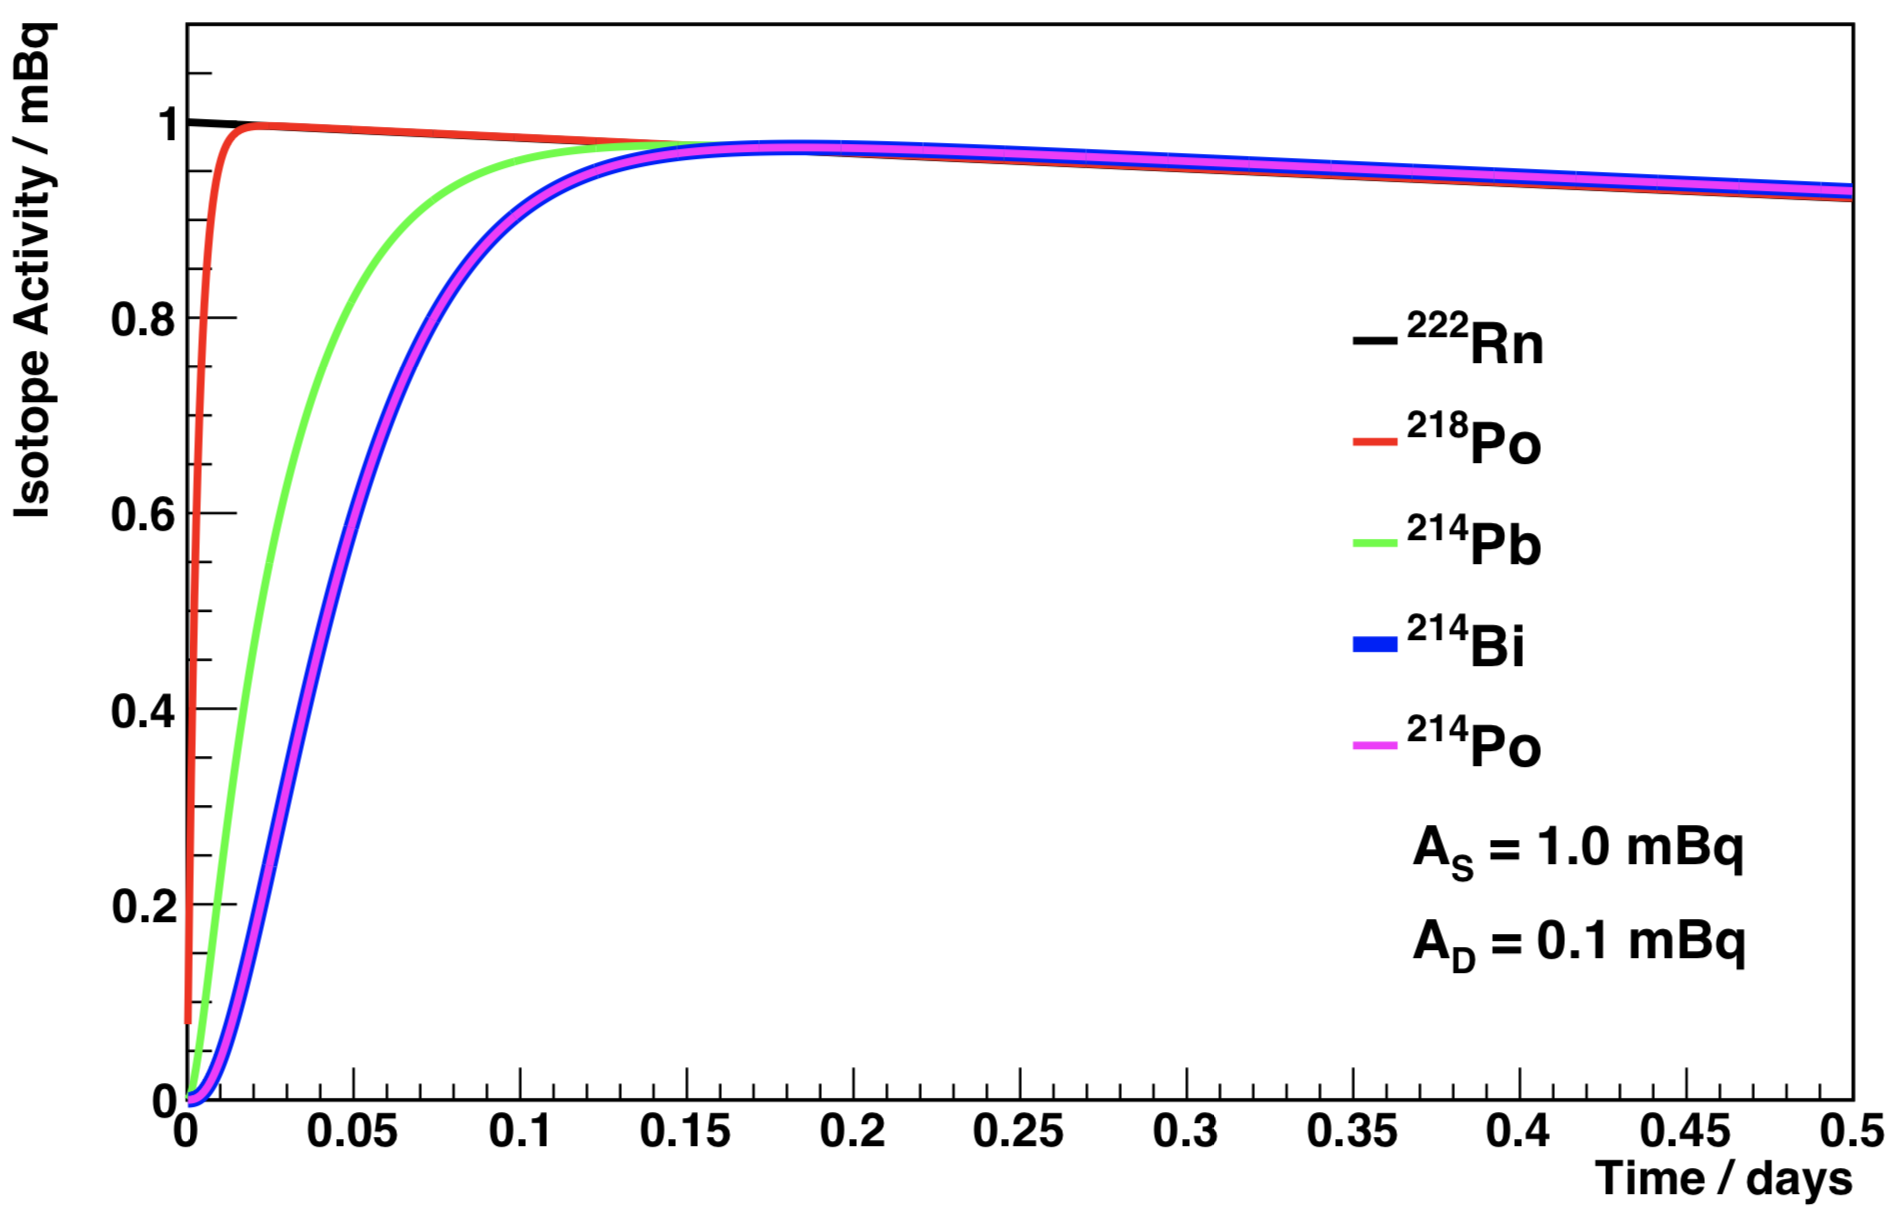
\includegraphics[scale=0.40]{Chapter_4/Figures/radon_chain_activities.png}
    \caption[The evolution of activities of the \RnTTT{} decay chain with respect to time under the starting condition of 1 mBq of \RnTTT{}.]
    {The evolution of activities of the \RnTTT{} decay chain with respect to time under the starting condition of 1 mBq of \RnTTT{}. $A_{D}$ represents the intrinsic background activity of the detector. Figure adapted from \cite{mott_2013}.}
    \label{fig:radon_chain_activity_evolution}
\end{figure}
%
Its important to note that the activity of \PoTOE{} quickly reaches an equilibrium with \RnTTT{}, whereas it takes $\sim4.5$ hours for \PoTOF{}. Hence, this slight delay needs to be taken into account if the emanation from a sample is transferred into the detector prior to equilibrium. Provided equilibrium is reached, the measured activity of both \PoTOE{} and \PoTOF{} will be equivalent to the activity of \RnTTT{}.


\newpage
\subsection{Electrostatic Detector}
\label{secsec:electrostatic_detector}

The electrostatic detector used in this work has been specially developed for the use of ELEGANT V and Super-Kamiokande experiments in measuring low-levels of radon \cite{CHOI2001177, MITSUDA2003414}. A detector with identical specifications developed by the same group was later acquired for SuperNEMO for background studies, as detailed in \cite{mott_2013}. Its design capability can measure radon activities to 1-2 mBq/\cubicmeter{}, 2 orders of magnitude improvement upon commercially available radon detectors. The schematics of the system are shown in figure \ref{fig:elecrostatic_detector}. 
%
\begin{figure}[h!]
    \centering
    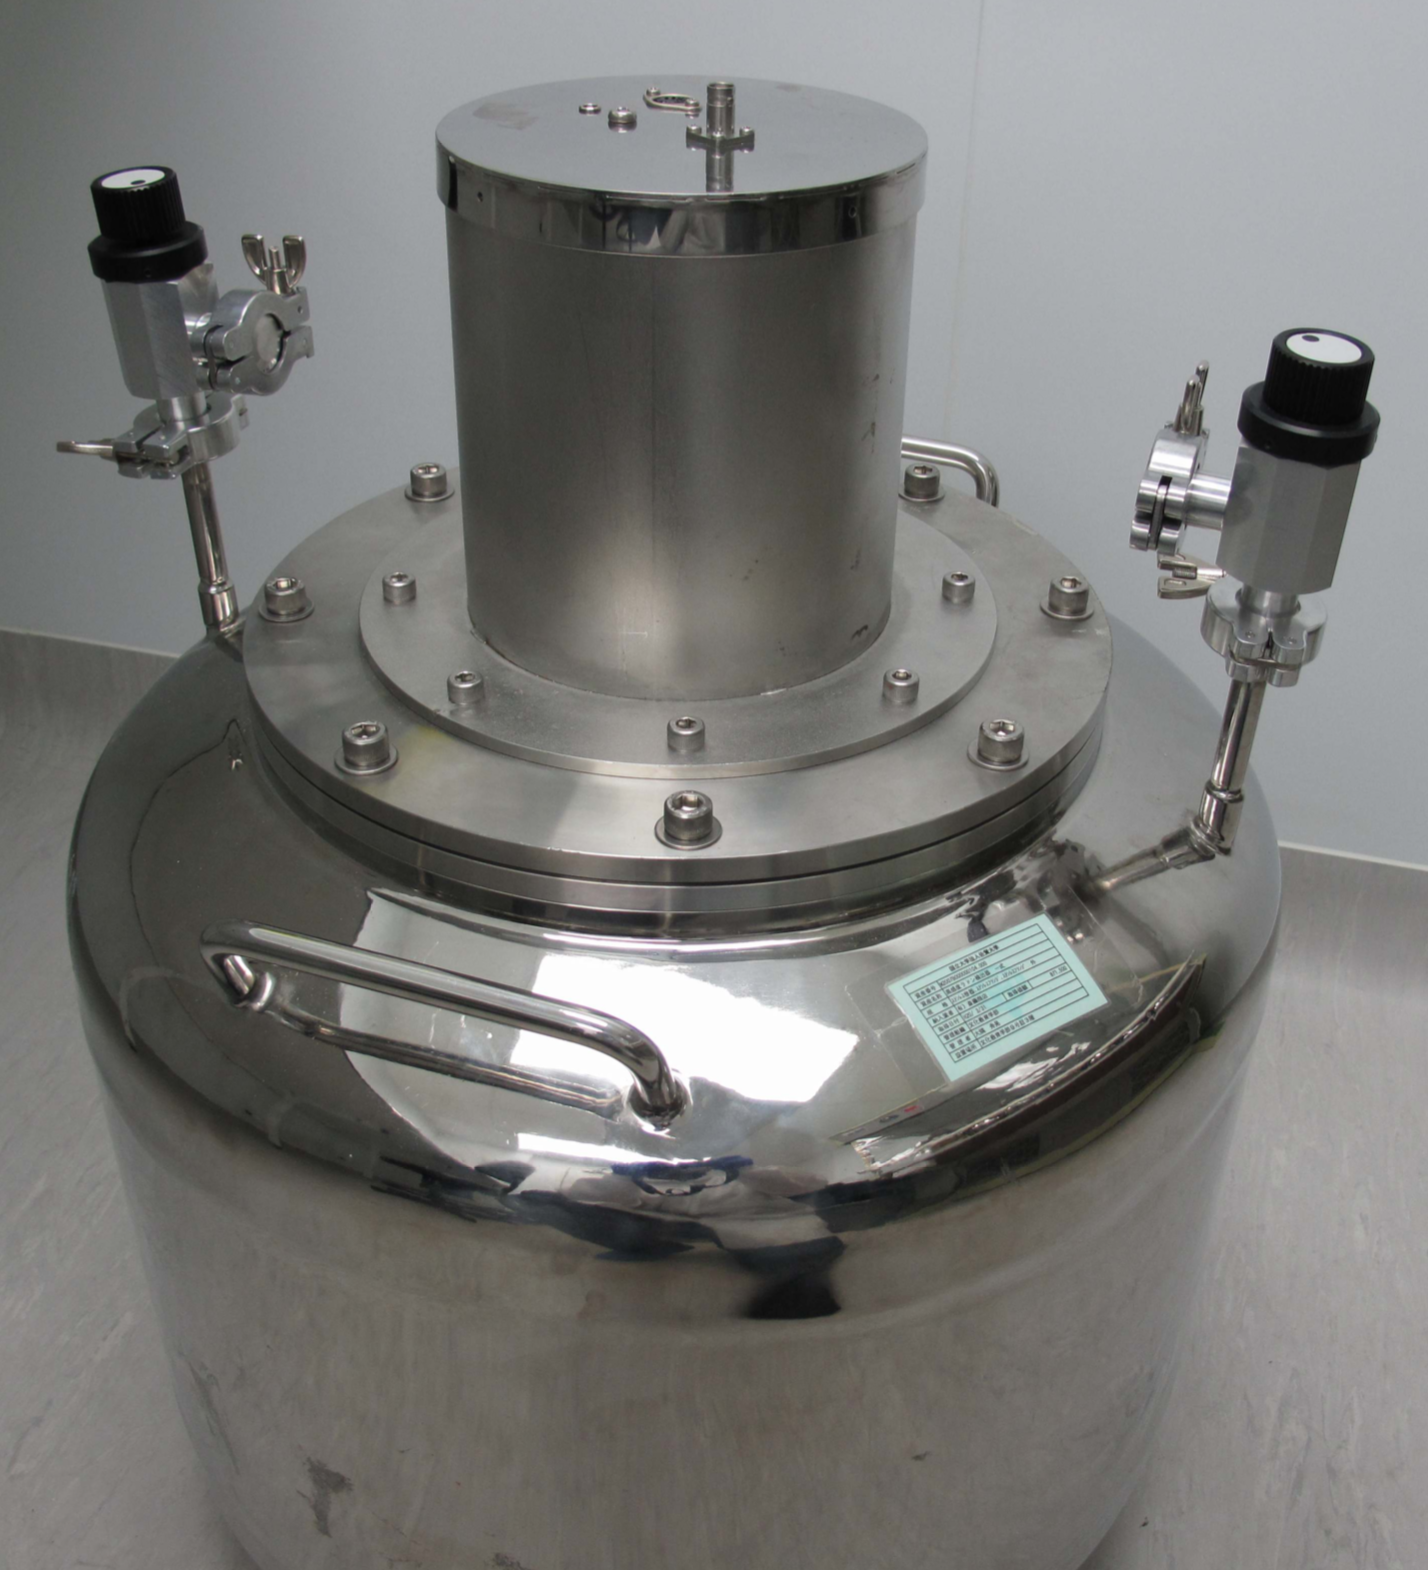
\includegraphics[scale=0.3]{Chapter_4/Figures/electrostatic_detector_1.png}
    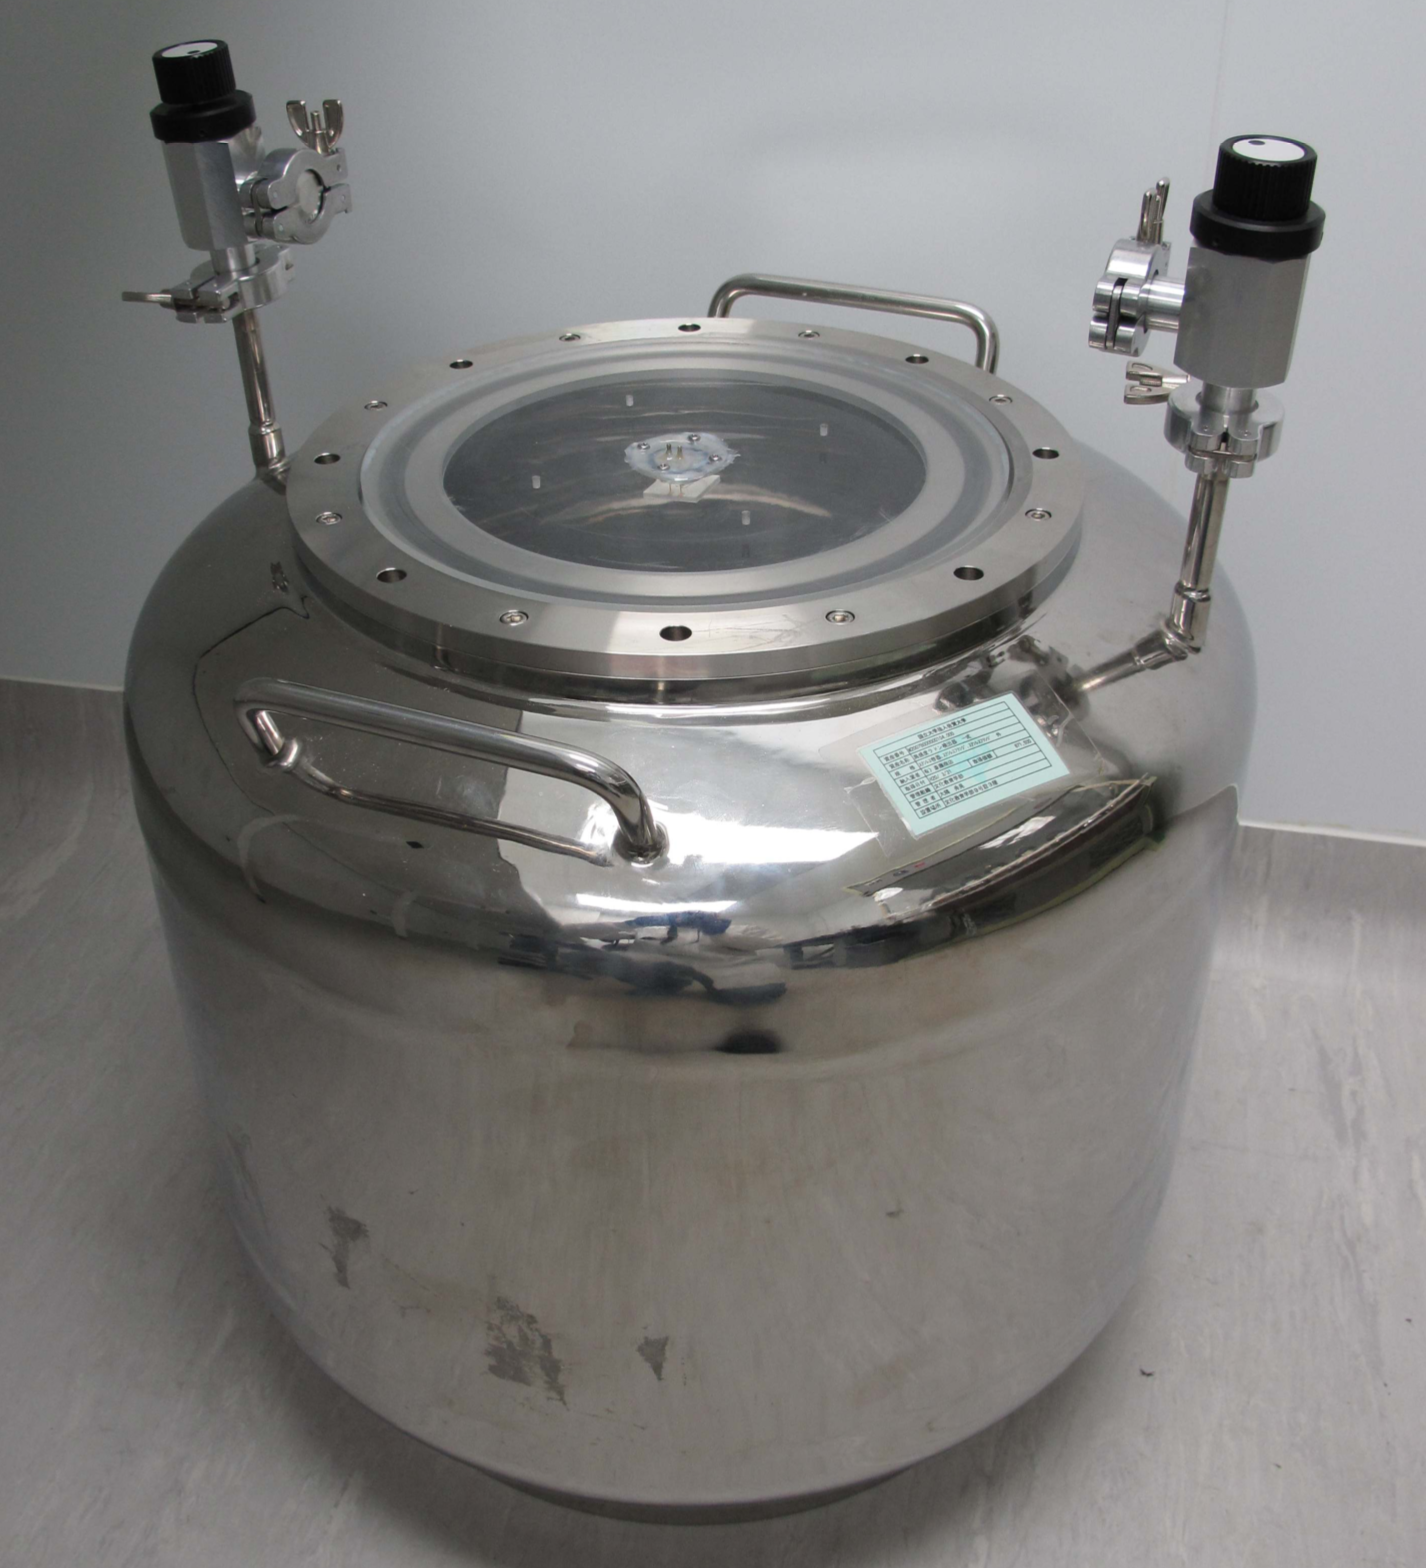
\includegraphics[scale=0.3]{Chapter_4/Figures/electrostatic_detector_2.png}
    \caption[Pictorial diagram of the electrostatic detector used for the radon emanation results published in this work.]
    {Pictorial diagram of the electrostatic detector used for the radon emanation results published in this work. Left shows the detector in full operational mode and the right shows it without its lid, where the feedthrough for the PIN-diode can be seen.}
    \label{fig:elecrostatic_detector}
    %----------
    \vspace{2cm}
    %----------
    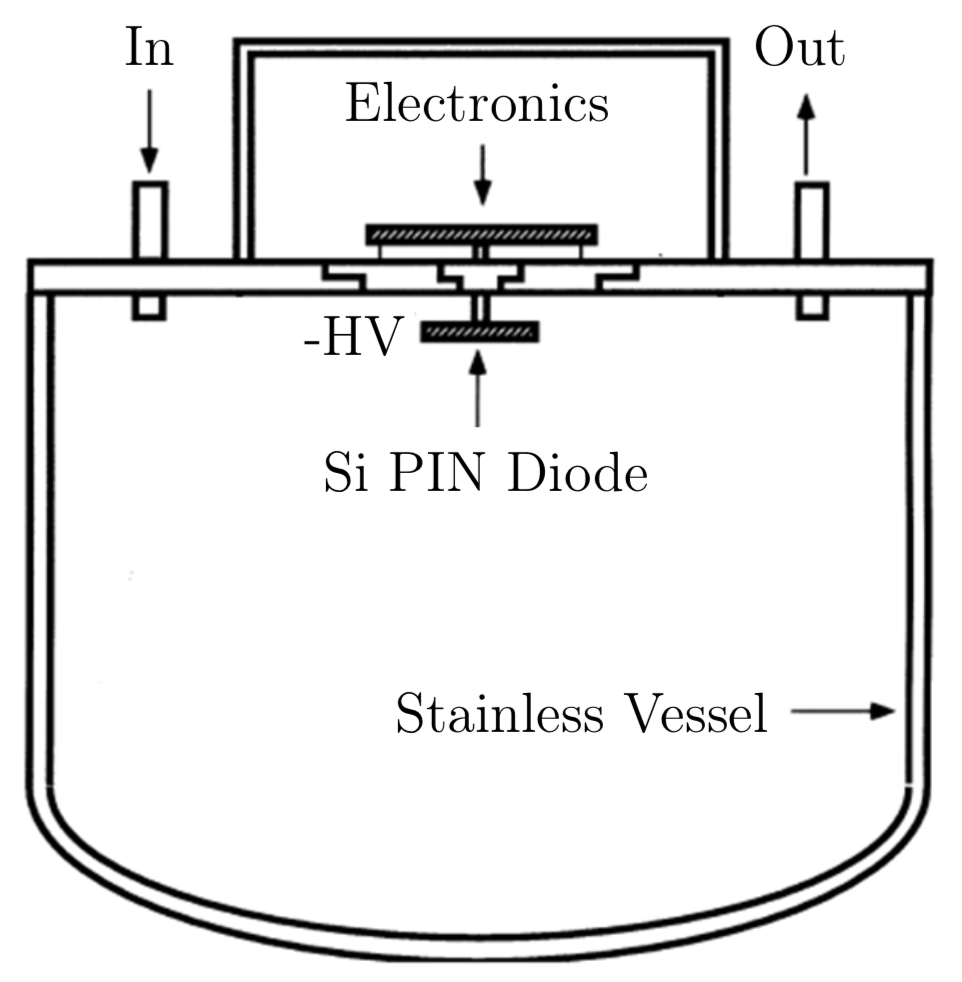
\includegraphics[scale=0.5]{Chapter_4/Figures/electrostatic_detector_schematic.png}
    \caption[A schematic diagram of the electrostatic detailing the electronics.]
    {A schematic diagram of the electrostatic detailing the electronics.}
    \label{fig:elecrostatic_detector_schematic}
\end{figure}
%

The simple design of the detector consists of an electro-polished stainless steel chamber with a 70 litre volume with a silicon PIN-diode attached to the top of the detector as shown schematically in figure \ref{fig:elecrostatic_detector_schematic}. The associated detector electronics are housed in the lid of the detector, separated from the measurement chamber by a sheet of perspex with a feedthrough for the PIN-diode. The detector has an inlet and an outlet valve for gas flow, all either metallic or have been coated with styrene butadiene rubber (SBR) to reduce the internal radon background that diffuse out or through material and into the detector volume. An electric field is generated inside the chamber by applying a negative high voltage (typically −1500 V) onto the PIN-diode.
 
In a standard operation, a sample is usually left to emanate for a set amount of time after which the gas content is transferred into the detection volume. The radon atoms decay within the volume result in daughter nuclei that are predominantly positively charged ions (\SI{87.3\pm1.6}{\percent} \cite{PAGELKOPF20031057}). These ions are effectively collected by the PIN-diode as a result of the applied electric field. The \alpha{} particles emitted from the \potoe{} and \potof{} ions are detected by the PIN-diode as they undergo \alpha{}-decay and are distinguished by the energies they deposit; \SI{6.1}{\mega\electronvolt} and \SI{7.9}{\mega\electronvolt}, respectively. 


\subsection{Detector Efficiency}
\label{sec:detector_efficiency}

Understanding the response of the detector to a known activity of radon is vital in modelling the detector response and correcting the measured activity for detector related efficiencies. In modelling this, a calibration source of \RaTTS{} (Pylon Electronics, RN-1025) with a known activity of 1.32 kBq was used. The source is designed to allow for gas flow through the material to transfer the emanated radon effectively into the detector volume, ensuring all of the radon to be exhausted.

The method used in calibrating the detector is sometimes referred to as the \textit{spike} method. The source volume is initially flushed out by the use of a helium carrier gas by around 10--100 times the volume of the source to ensure all of the radon is exhausted thoroughly. The volume is then sealed for a set amount of time to allow for a set amount of radon to build up. In a typical calibration, helium is used as a carrier gas to move 2.5 Bq of radon into the detector. The background spectrum of the electrostatic detector without and with a typical calibration source injection is shown in figure \ref{fig:background_calibration_spectrum}. 
%
\begin{figure}[hb!]
    \centering
    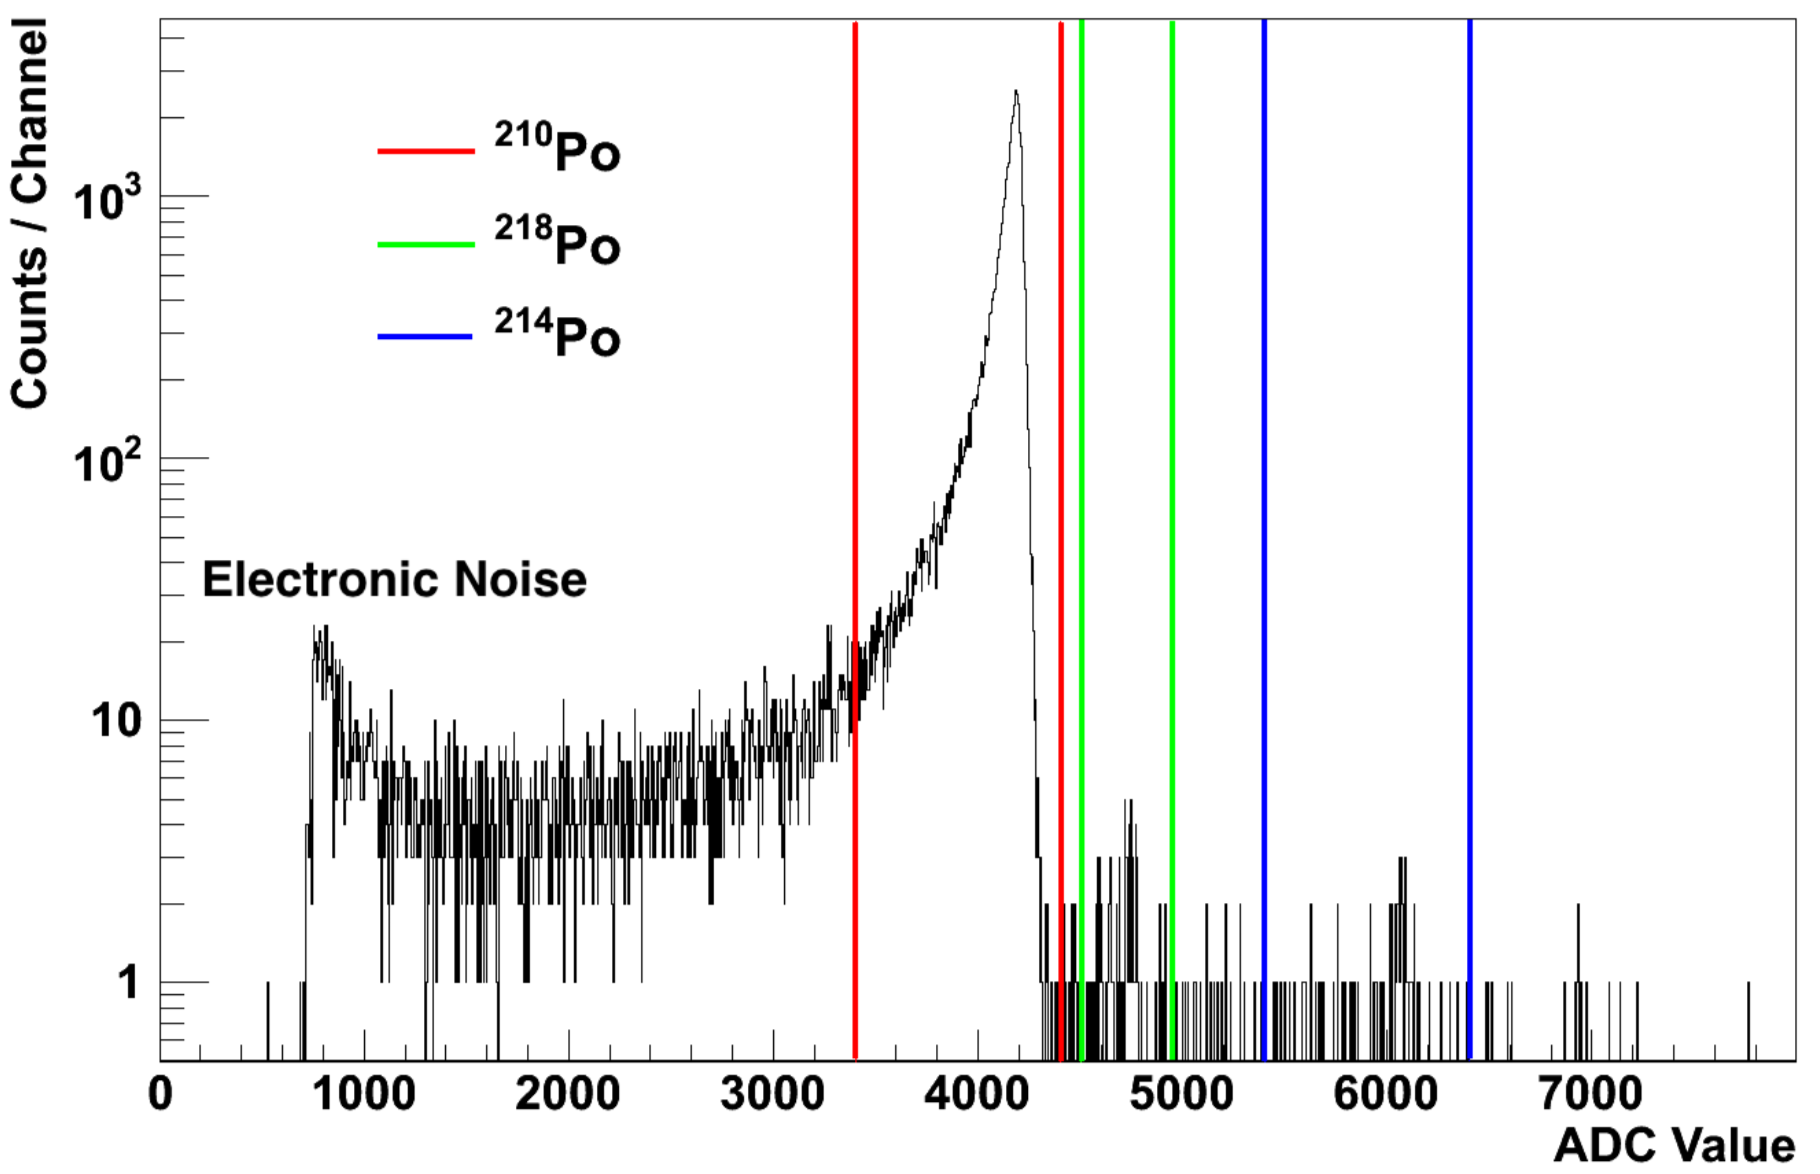
\includegraphics[scale=0.23]{Chapter_4/Figures/background_spectra.png}
    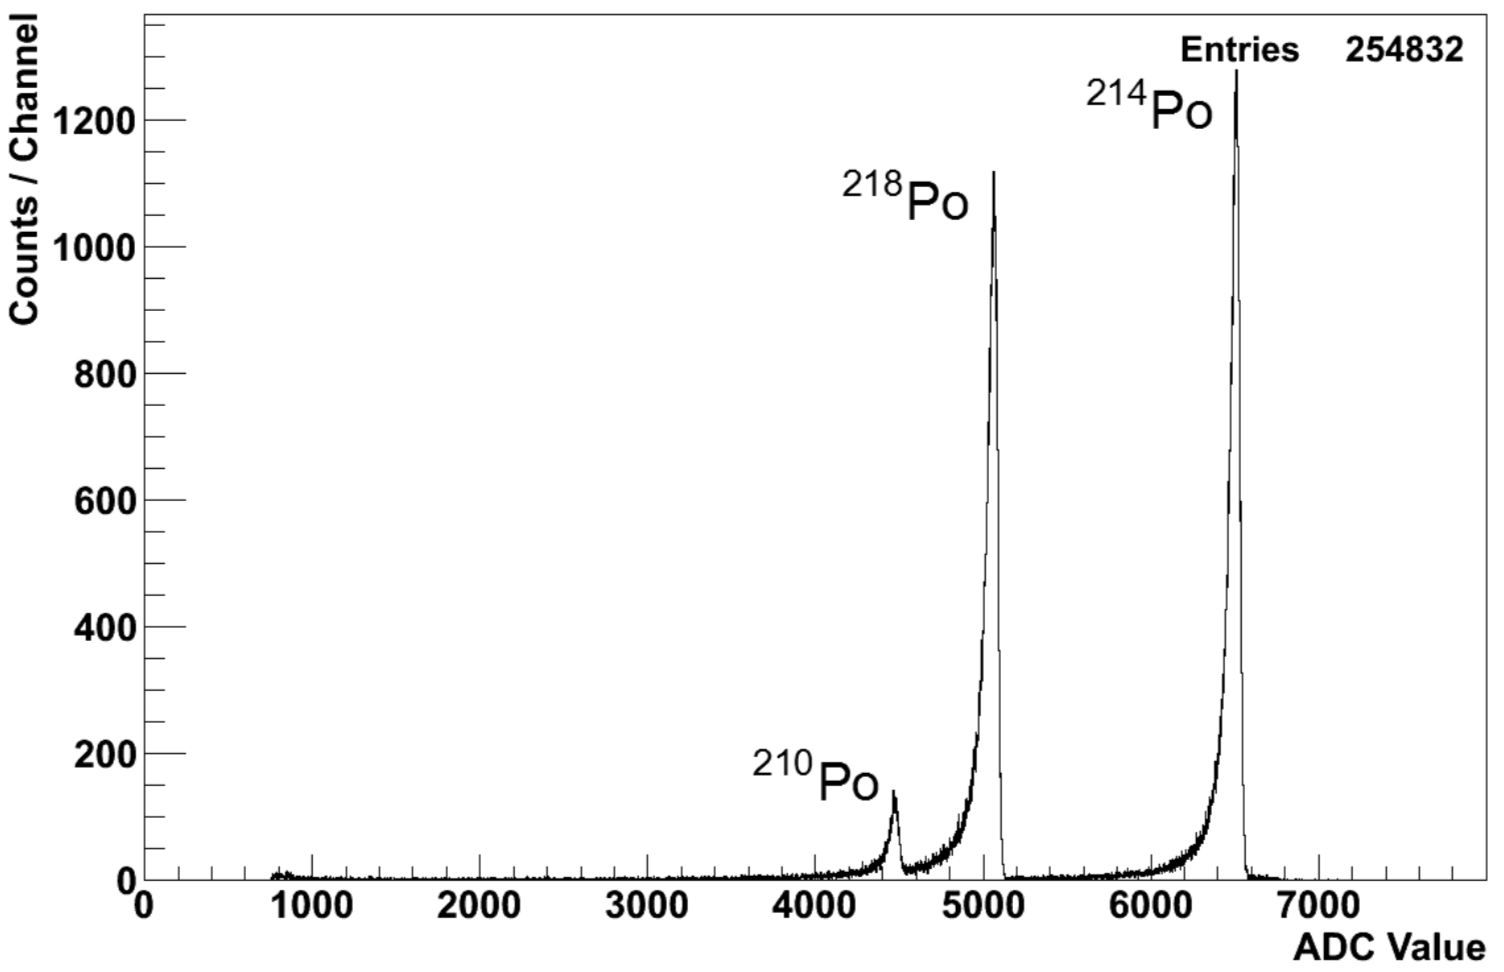
\includegraphics[scale=0.28]{Chapter_4/Figures/calibration_spectra.png}
    \caption[Spectrum from the electrostatic detector without and with 2.5 Bq of the calibration present.]
    {Spectrum from the electrostatic detector without (left) and with (right) 2.5 Bq of the calibration source present. The spectral peaks of \PoTOZ{}, \PoTOE{} and \PoTOF{} are displayed from left to right. The red, green and blue windows are used to select regions of the spectrum associated with the isotopes of interest for further analysis.}
    \label{fig:background_calibration_spectrum}
\end{figure}
%

In an event where the ionised radon progeny attaches onto the PIN-diode and undergoes \alpha{}-decay, the kinetic energy carried by the \alpha{}-particle can be identified by the induced amplitude of the signal. The energy resolution of these detectors is such that the peaks observed for the three isotopes of polonium are clearly visible after the source injection. Although some \PoTOZ{} is present as a result of the calibration source, the majority of its observed activity is as a result of residual exposure of the PIN-diode and its longer half-life of $\sim140$ days. This residual activity is more apparent on the background spectrum of the detector prior to source injection, as seen on the left in figure \ref{fig:background_calibration_spectrum}. Although one may naively think that the peaks of \PoTOF{} and \PoTOF{} should be identical in activity (counts), this is often not the case. This apparent difference in efficiency is thought to be as a result of \PoTOF{} decay taking place after multiple intermediary isotopic decays. The intermediate isotopes \PbTOF{} and \BiTOE{} are assumed to be predominantly created as ions and as a result are collected by the PIN-diode. This results in more \PbTOF{} either on the PIN-diode or close to the PIN-diode, reducing the probability of neutralisation, which often takes place under trace amounts of impurities, such as nitrous oxide (N$_{2}$O). Although \alpha{}-decay counts from both \PoTOE{} and \PoTOF{} can be used to reconstruct the radon activity, the activities quoted are from \PoTOF{} due to its higher detection efficiency. Furthermore, despite the energy resolution, some overlap between the \PoTOE{} and \PoTOZ{} peak is unavoidable.
%
\begin{figure}[b!]
    \centering
    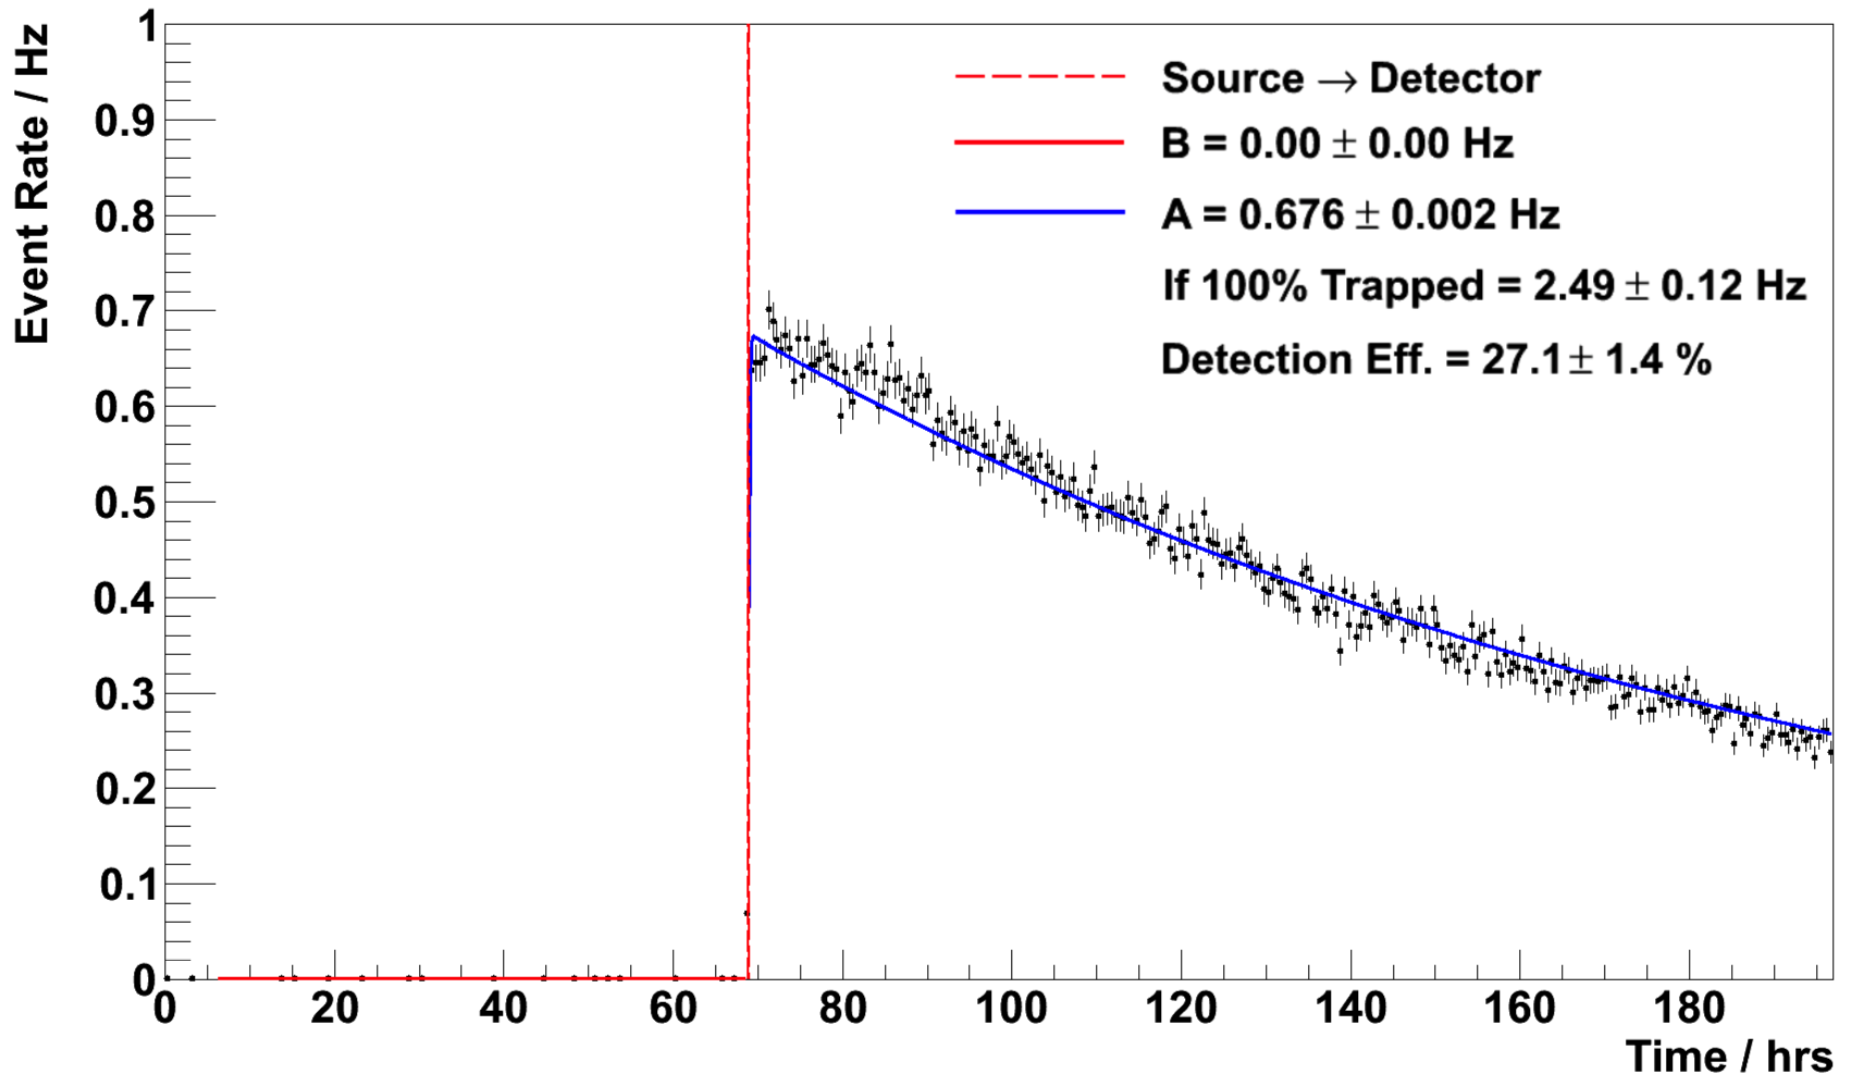
\includegraphics[scale=0.23]{Chapter_4/Figures/Po_218_Calibration.png}
    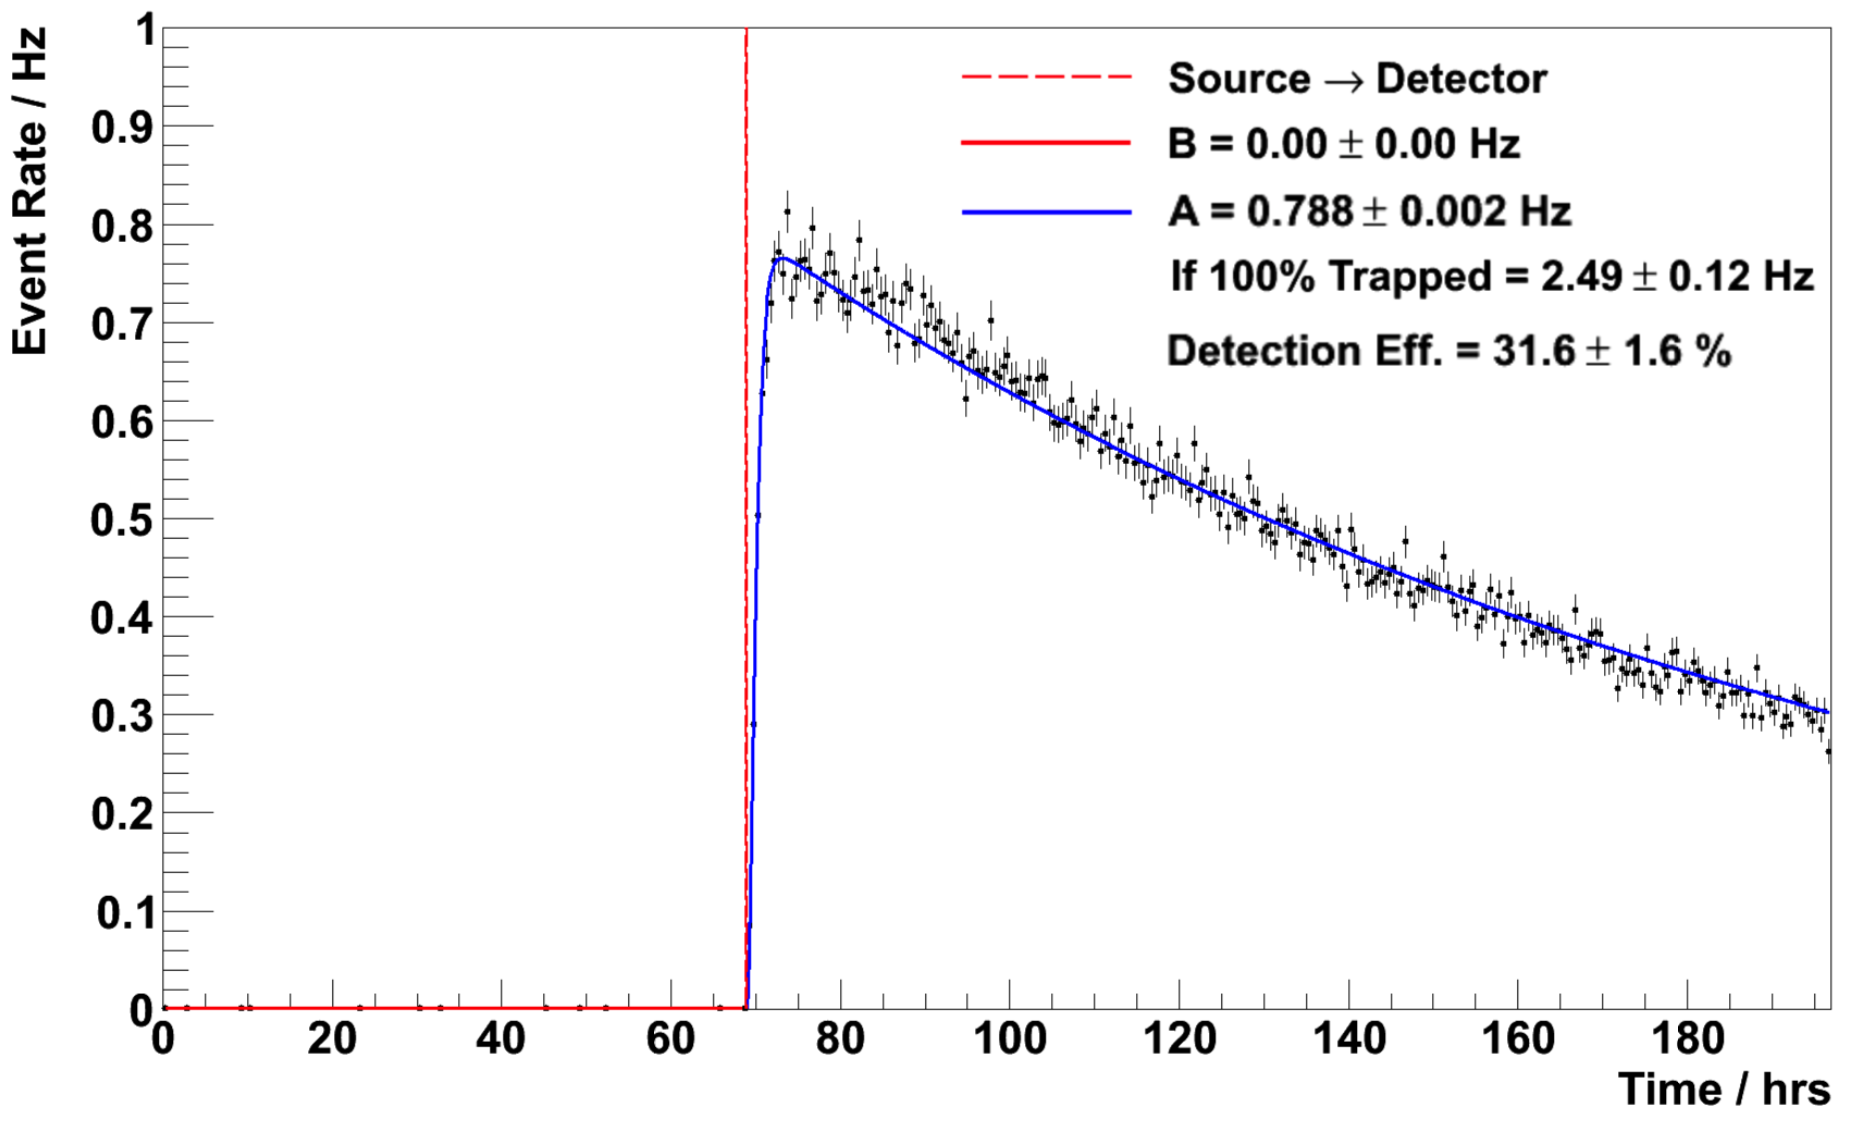
\includegraphics[scale=0.23]{Chapter_4/Figures/Po_214_Calibration.png}
    \caption[\PoTOE{} and \PoTOF{} event rates for a calibration injection of 2.5 Bq of radon into the detector via a helium carrier gas.]
    {\PoTOE{} (left) and \PoTOF{} (right) event rates for a calibration injection of 2.5 Bq of radon into the detector via a helium carrier gas. The fitted black line shows the expected response for the given isotope with all half-lives fixed to their known values.}
    \label{fig:calibration_decay_fit}
\end{figure}
%

To calculate the detection efficiency, the peaks of \PoTOE{} and \PoTOF{} are initially selected with predetermined windows, and their respective activities are fit using decay equations derived from equation \ref{eq:isotopic_chance_in_chain} and shown in detail in \cite{mott_2013}. A typical result from a 2.5 Bq of radon injection into the detector is shown in figure \ref{fig:calibration_decay_fit}. The detection efficiency was then calculated as $27.1\pm1.4\%$ and $31.6\pm1.6\%$ for \PoTOE{} and \PoTOF{}, respectively. Its important to note that the maximum detection efficiency achievable using this technique is 50\%, as half of the \alpha{}-particles are emitted away from the PIN-diode and hence never measured. 


\subsection{Detector Background Measurement}
\label{secsec:concentration_line}

The sensitivity of the detector and the measured activities are not limited to the efficiency of the detector alone but also the detector background rate. In general, a typical measurement would include a measurement of the background rate of the detector $\sim5$ days prior to the transfer. This background rate is then subtracted from the measured activity post transfer. Additionally, much longer background measurements are performed periodically to ensure the stability of the detector. In such measurements, the detector is fully sealed to both the gas line and the environment and the radon activity is continuously measured. The energy spectrum from this type of run is different to that of a calibration run as can be seen in figure \ref{fig:detector_background_spectrum}.
%
\begin{figure}[b!]
    \centering
    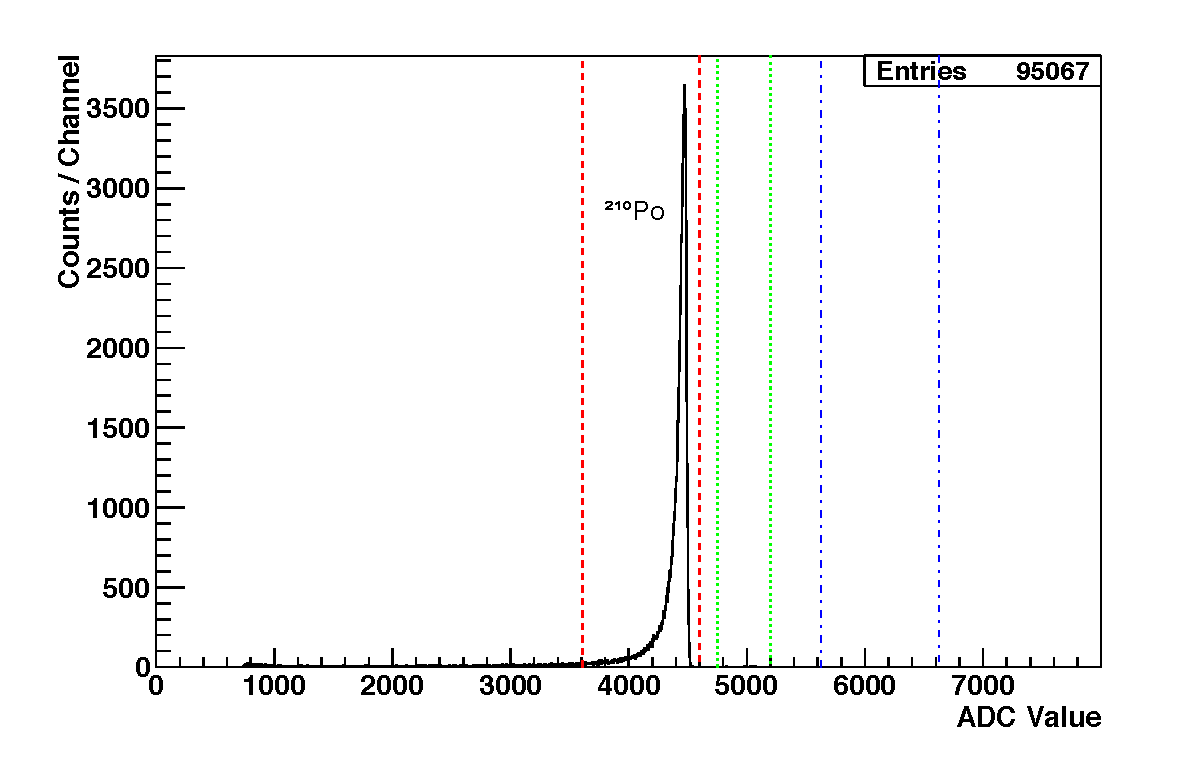
\includegraphics[scale=0.43]{Chapter_4/Figures/det_background/Spectrum_det_background.pdf}
    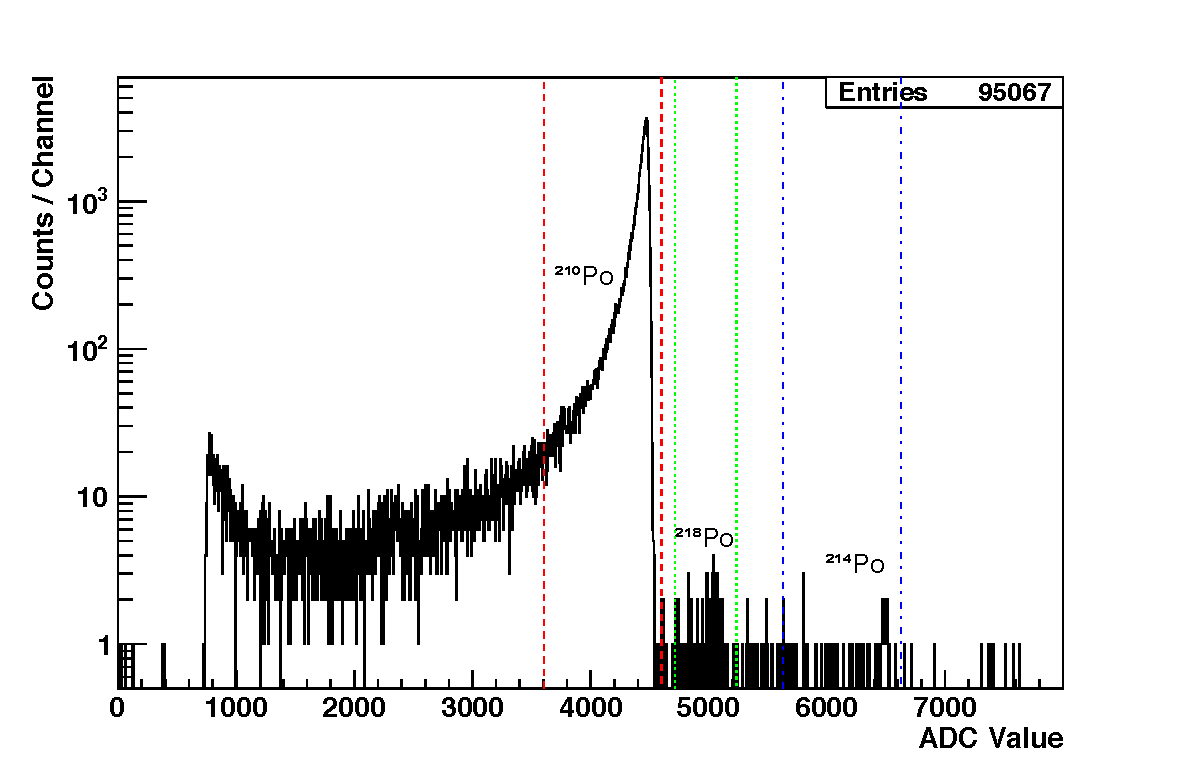
\includegraphics[scale=0.43]{Chapter_4/Figures/det_background/LogSpectrum_det_background.pdf}
    \caption[Energy spectrum of a long radon emanation detector backgrounds showing the peaks of \PoTOZ{}, \PoTOE{} and \PoTOF{}.]
    {Energy spectrum of a long detector background measurement with linear and logged y-axis. The peaks of \PoTOZ{}, \PoTOE{} and \PoTOF{} are displayed accordingly.}
    \label{fig:detector_background_spectrum}
\end{figure}
%

The observed spectrum is similar to that of a typical material measurement with a dominant \PoTOZ{} that has accumulated onto the PIN-diode from prior calibration runs. The \PoTOE{} and \PoTOF{} peaks are visible on a logarithmic scale and a smaller peak from \PoTOT{} at 8.9 MeV from the thoron chain is also visible. The peaks are selected with pre-determined windows as shown by the vertical lines on figure \ref{fig:detector_background_spectrum} and the activity of \PoTOF{}, along with that of \PoTOZ{} is shown in figure \ref{fig:detector_background_rates}. 
%
\begin{figure}[t!]
    \centering
    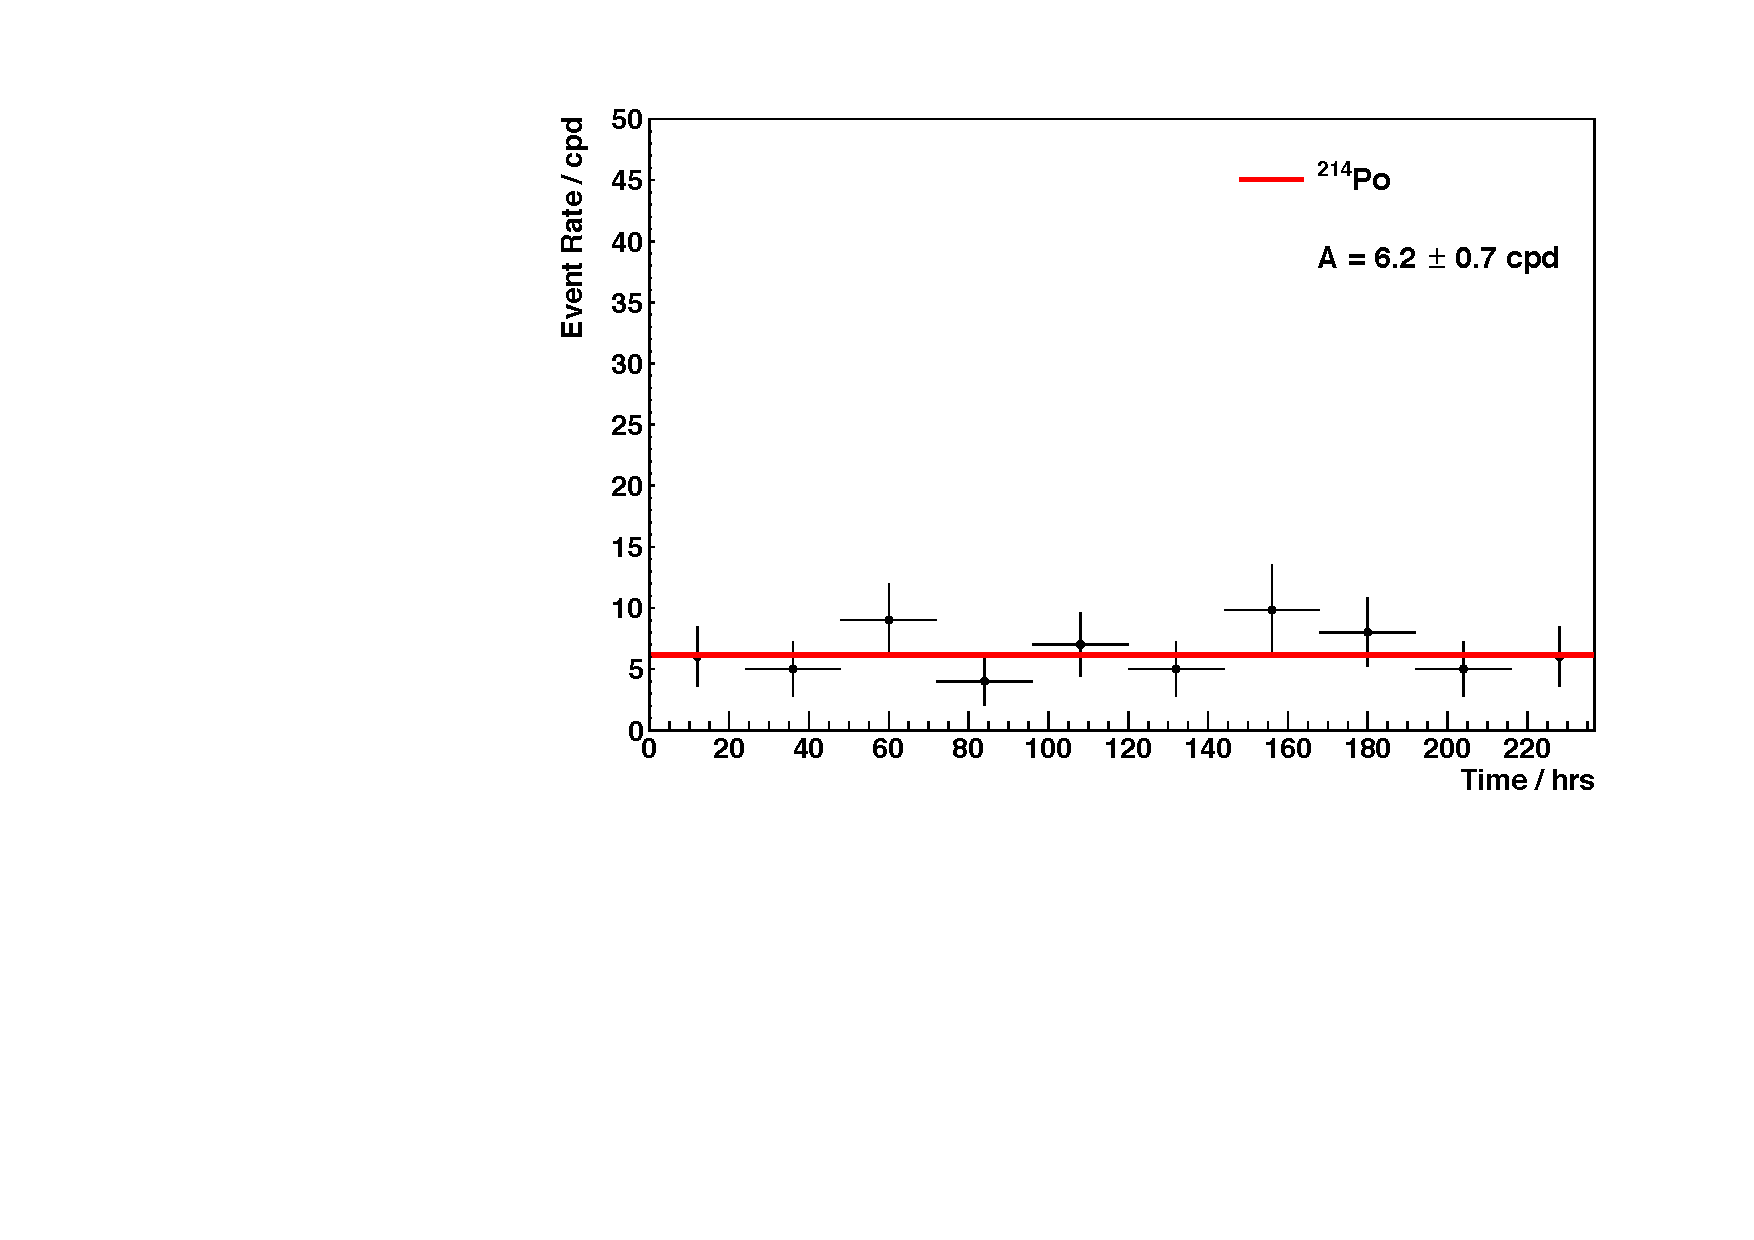
\includegraphics[scale=0.43]{Chapter_4/Figures/det_background/Po214_det_background.pdf}
    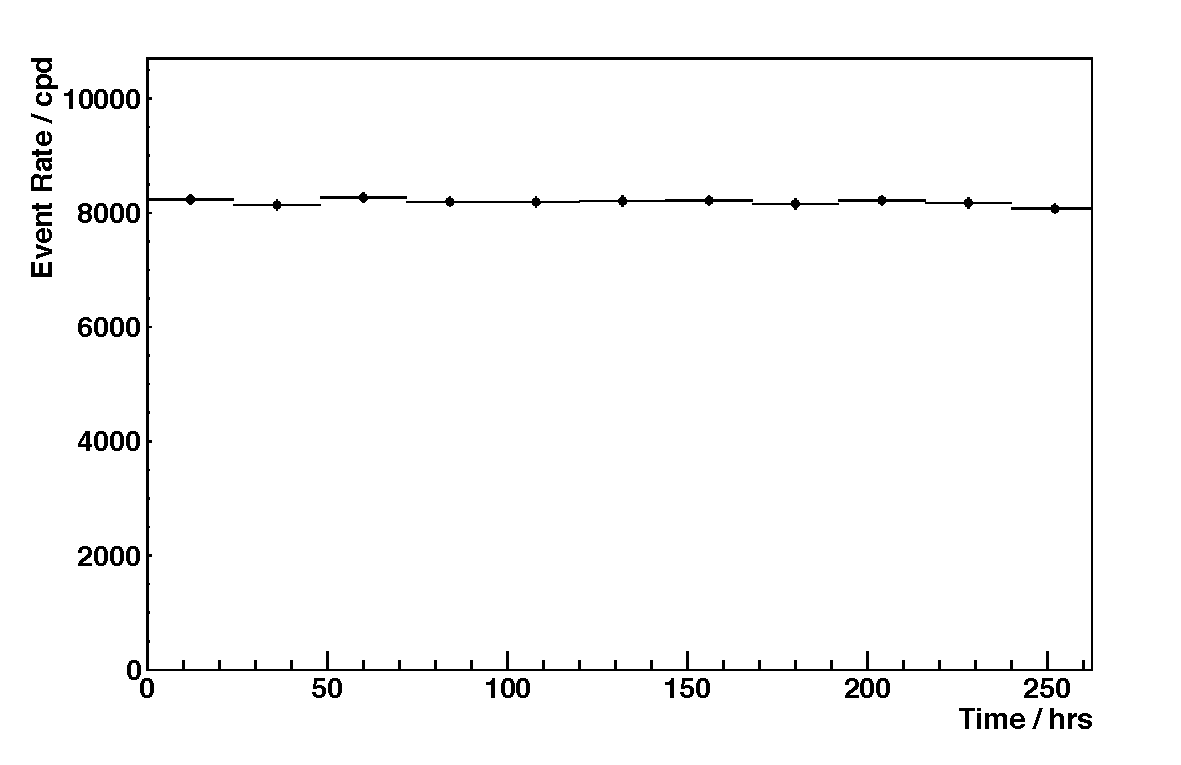
\includegraphics[scale=0.43]{Chapter_4/Figures/det_background/Po210_det_background.pdf}
    \caption[\PoTOF{} and \PoTOZ{} event rates for a typical background measurement run.]
    {\PoTOF{} (left) and \PoTOZ{} (right) event rates for a typical background measurement run. The \PoTOF{} rate shows a relatively low background level, whereas the \PoTOZ{} shows the stability of the detector.}
    \label{fig:detector_background_rates}
\end{figure}
%

The inferred \PoTOF{} rate, which is the primary channel to reconstruct the radon emanation rate shows an averaged daily rate of $6.2\pm{}0.7$\,counts-per-day (cpd). The detector in this measurement is initially flushed thoroughly and filled with helium gas, so by using the detector efficiency of 31.6\% for \PoTOF{}, the intrinsic activity of the detector is determined to be $0.20\pm0.02$\,mBq. Besides the \PoTOF{} rate, the \PoTOZ{} rate is also measured as shown in figure \ref{fig:detector_background_rates}. Although this does not inform on the radon activity, it is a useful measure in checking the stability of the detector and the DAQ over time, as this rate is expected to be constant over a measurement period. 

\subsection{System Design and Schematics}
\label{secsec:system_design_schematics}

The electrostatic detector as detailed in the previous sections is part of a large system that handles gas flow in and out of the sample chamber and detector. A pictorial and a schematic diagram of the design is shown in figures \ref{fig:detector_design_picture} \& \ref{fig:detector_design_schematic}.
%
\begin{figure}[]
    \centering
    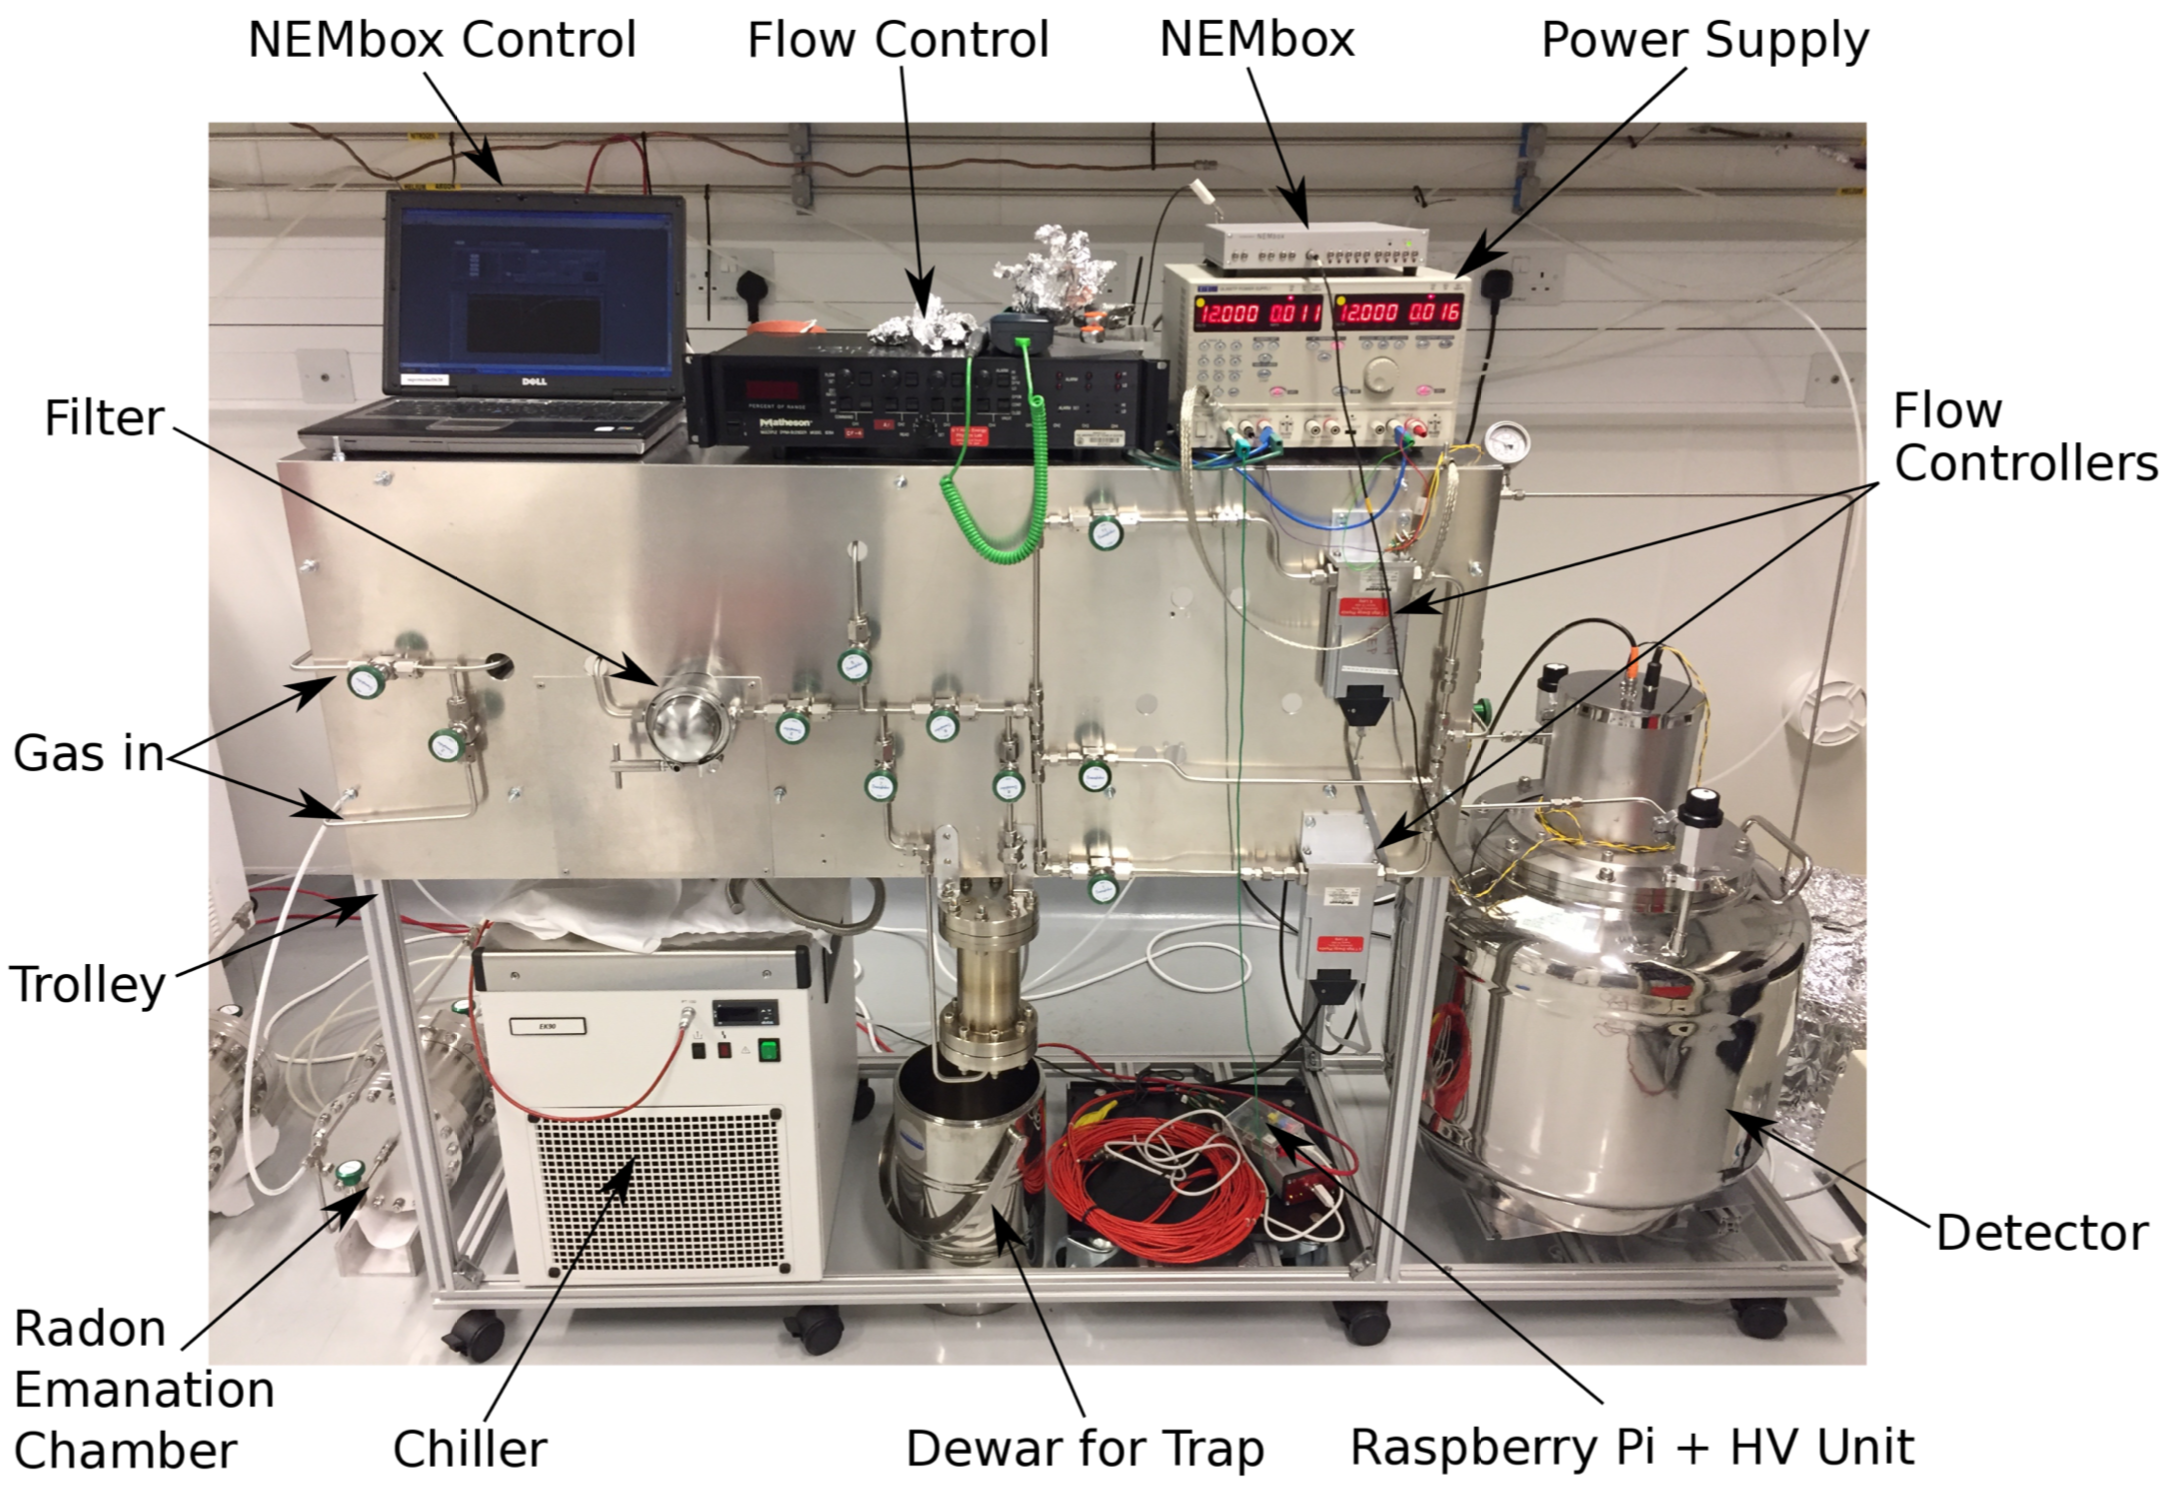
\includegraphics[scale=0.4]{Chapter_4/Figures/radon_system_design.png}
    \caption[A pictorial diagram of the UCL radon emanation system with key components highlighted.]
    {A pictorial diagram of the UCL radon emanation system with key components highlighted.}
    \label{fig:detector_design_picture}
\end{figure}
%
%
\begin{figure}[]
    \centering
    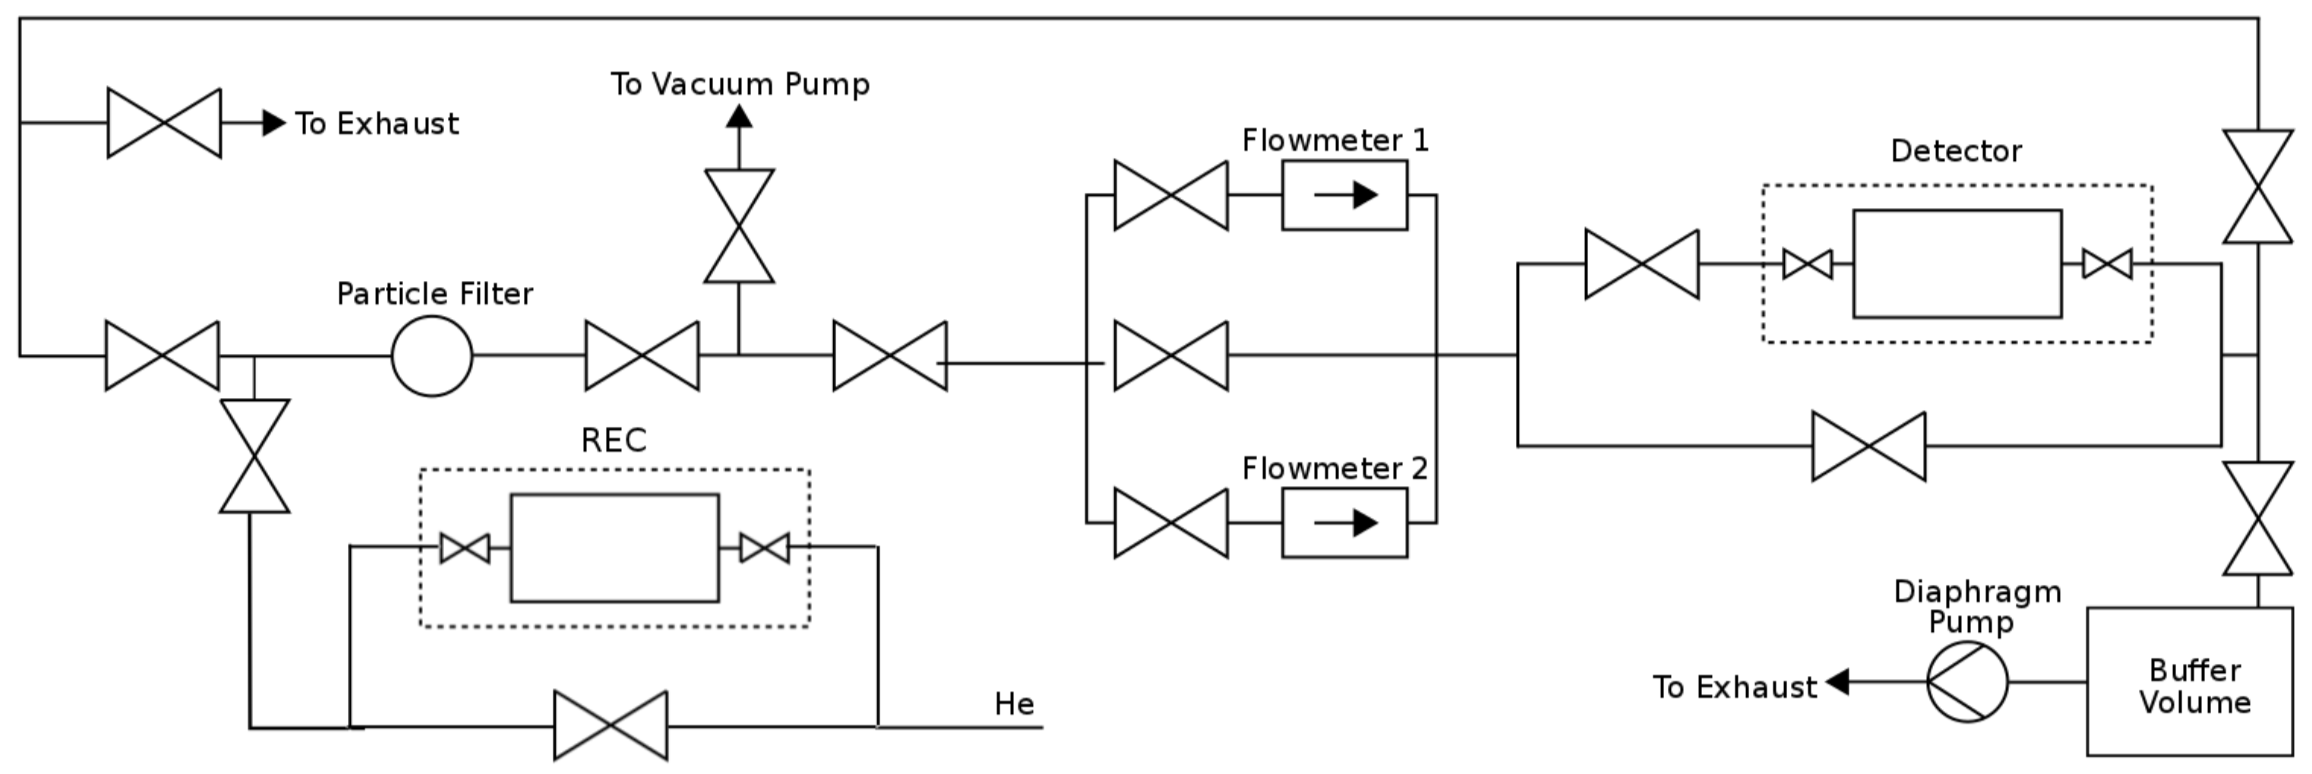
\includegraphics[scale=0.38]{Chapter_4/Figures/radon_system_pid.png}
    \caption[A schematic diagram of the UCL radon emanation system.]
    {A schematic diagram of the UCL radon emanation system.}
    \label{fig:detector_design_schematic}
\end{figure}
%

The system is design to facilitate a high degree of flexibility in operation. The carrier gas enters from the location marked as \textit{He} and can either flow through the radon emanation chamber (REC) or by-pass the chamber; crucial for calibration source injection or flushing the system without impacting the source emanation with the REC. Although helium has been used as the primary gas carrier, nitrogen can also be injected through the same flow path. Prior to entry, the gas is initially passed through an activated charcoal trap stored in an ultra-low temperate freezer (193 K) with 0.5 micron stainless steel particulate filters fitted on both ends to reduce particulate contamination. The charcoal trap scrubs the radon generated from the cylinders of the gas carriers to supply radon-free gas into the entire system. The carrier gas is then directed by a series of valves, with a flow meter determining the flow rate. All pipework is made from stainless steel and all valves are fully metallic, which reduces radon emanation.

The system operates two 2.7 L stainless steel chambers as the emanation media, as shown pictorially in figure \ref{fig:detector_chamber}. Once the sample is sealed inside the chamber, the chamber is flushed thoroughly to remove any ambient radon trapped inside and checked for leaks using a helium leak detector (GasCheck Tesla Helium Leak Detector)---ensuring no leaks above 10$^{−6}$ cc/s is observable. The larger detector volume and the small chamber volume allow a single step transfer process, where helium gas is flushed through the emanation chamber, carrying the emanated radon from the sample within the chamber directly into the detector. A carrier gas volume of ten times the chamber volume is used in this process to ensure a near 100\% transfer efficiency from the chamber into the detector. This mode of operation has been the primary way samples were screened for LZ.
%
\begin{figure}[]
    \centering
    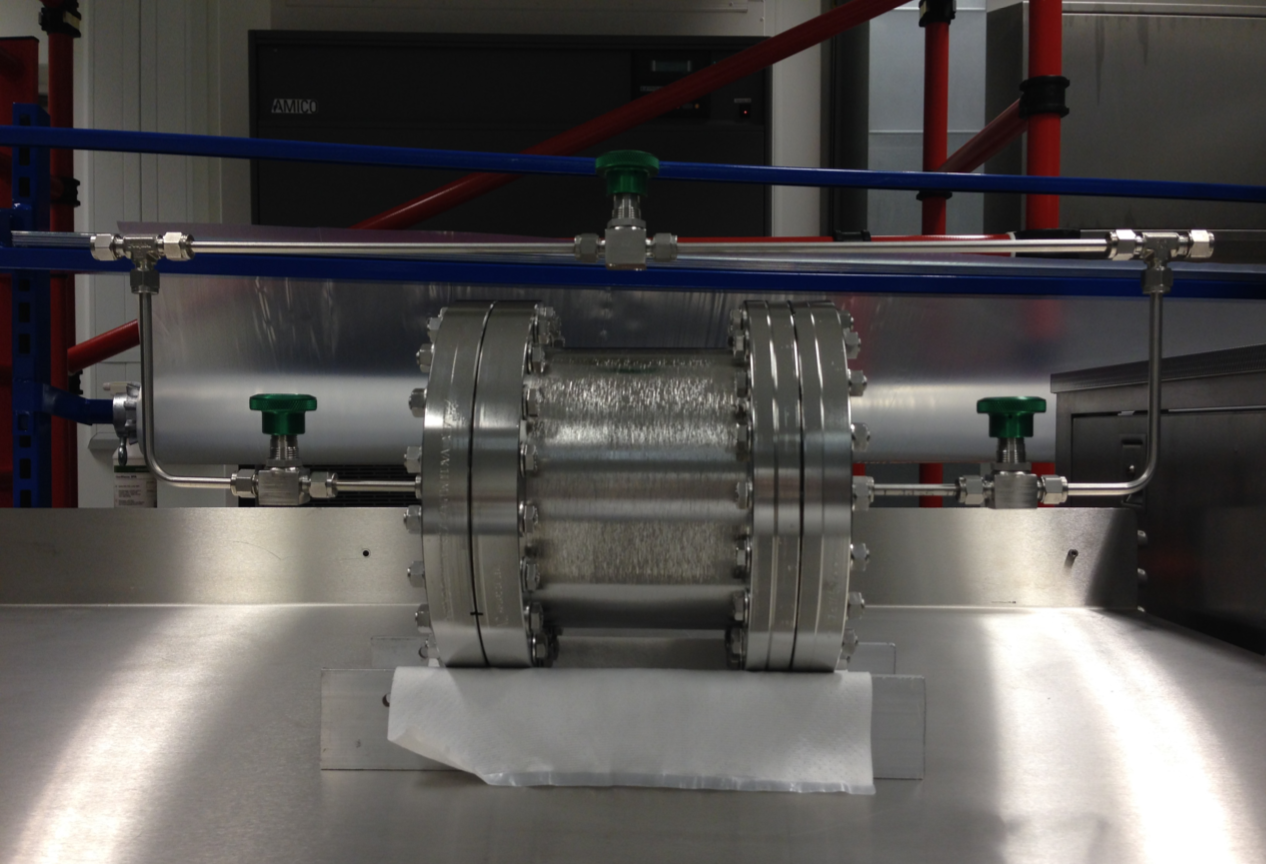
\includegraphics[scale=0.4]{Chapter_4/Figures/radon_system_chamber.png}
    \caption[A pictorial diagram of the 2.7 L stainless steel radon emanation chamber used to house samples for emanation.]
    {A pictorial diagram of the 2.7 L stainless steel radon emanation chamber used to house samples for emanation.}
    \label{fig:detector_chamber}
\end{figure}
%

A second mode of operation for the system uses 57\,g of activated carbon (a synthetic charcoal sourced from Carbo-Act International \cite{Pushkin:2018wdl}) as a radon collection trap. In larger emanation volumes, the radon is initially absorbed into the cooled trap while the carrier gas passes through. The trap is then heated to release the radon and the carrier gas is then used to transfer the concentrated radon into the detector volume. The trapping efficiency for this setup has been measured to be $\approx 93$\% at 248\,K \cite{xin_2017}.


%%------------------------------$$
\section{Radon Emanation Measurements for LZ}
\label{sec:uclradon}
%%------------------------------$$

Screening key components of the LZ detector that are in direct contact with the xenon circulation system for radon emanation has been one of the primary focal points in the LZ screening campaign. The UCL radon emanation system has been used extensively for several of these key measurements; including various PMT bases that are located inside the ICV and the TPC, the raw titanium and titanium welding used for the cryostats and several other structural segments with the ICV, and various other items. This section will highlight some of these results in detail.


\subsection{PMT Bases}
\label{secsec:pmt_base_emanation}

The LZ detector will use a total of 500 3", 39 2" and 94 1" PMT bases, all of which reside in the xenon volume of the detector. The components used in these bases are mostly (both in mass and area) made up of Cirlex (Kapton) printed circuit boards (PCBs), solder, capacitors, resistors and receptacles; together adding up to a considerable surface area within the xenon. Assays of these individual components have previously been conducted with \gamma{}-screening and radon emanation to build a \textit{bottom-up} model of the expected radon from the fully assembled bases. The solder and the receptacles were excluded as they yielded low \UTTEe{} activities with \gamma-screening; and emanation results from the other components yielded a \textit{bottom-up} approximation of 1.01 mBq for all bases used in LZ. This corresponds to 1.65 \micro{}Bq and 1.25 \micro{}Bq per a 3" and 1" base respectively. The pictorial diagram of the 1" and 3" bases used in this study are shown in figure \ref{fig:1_and_3_inch_bases}.
%
\begin{figure}[b]
    \centering
    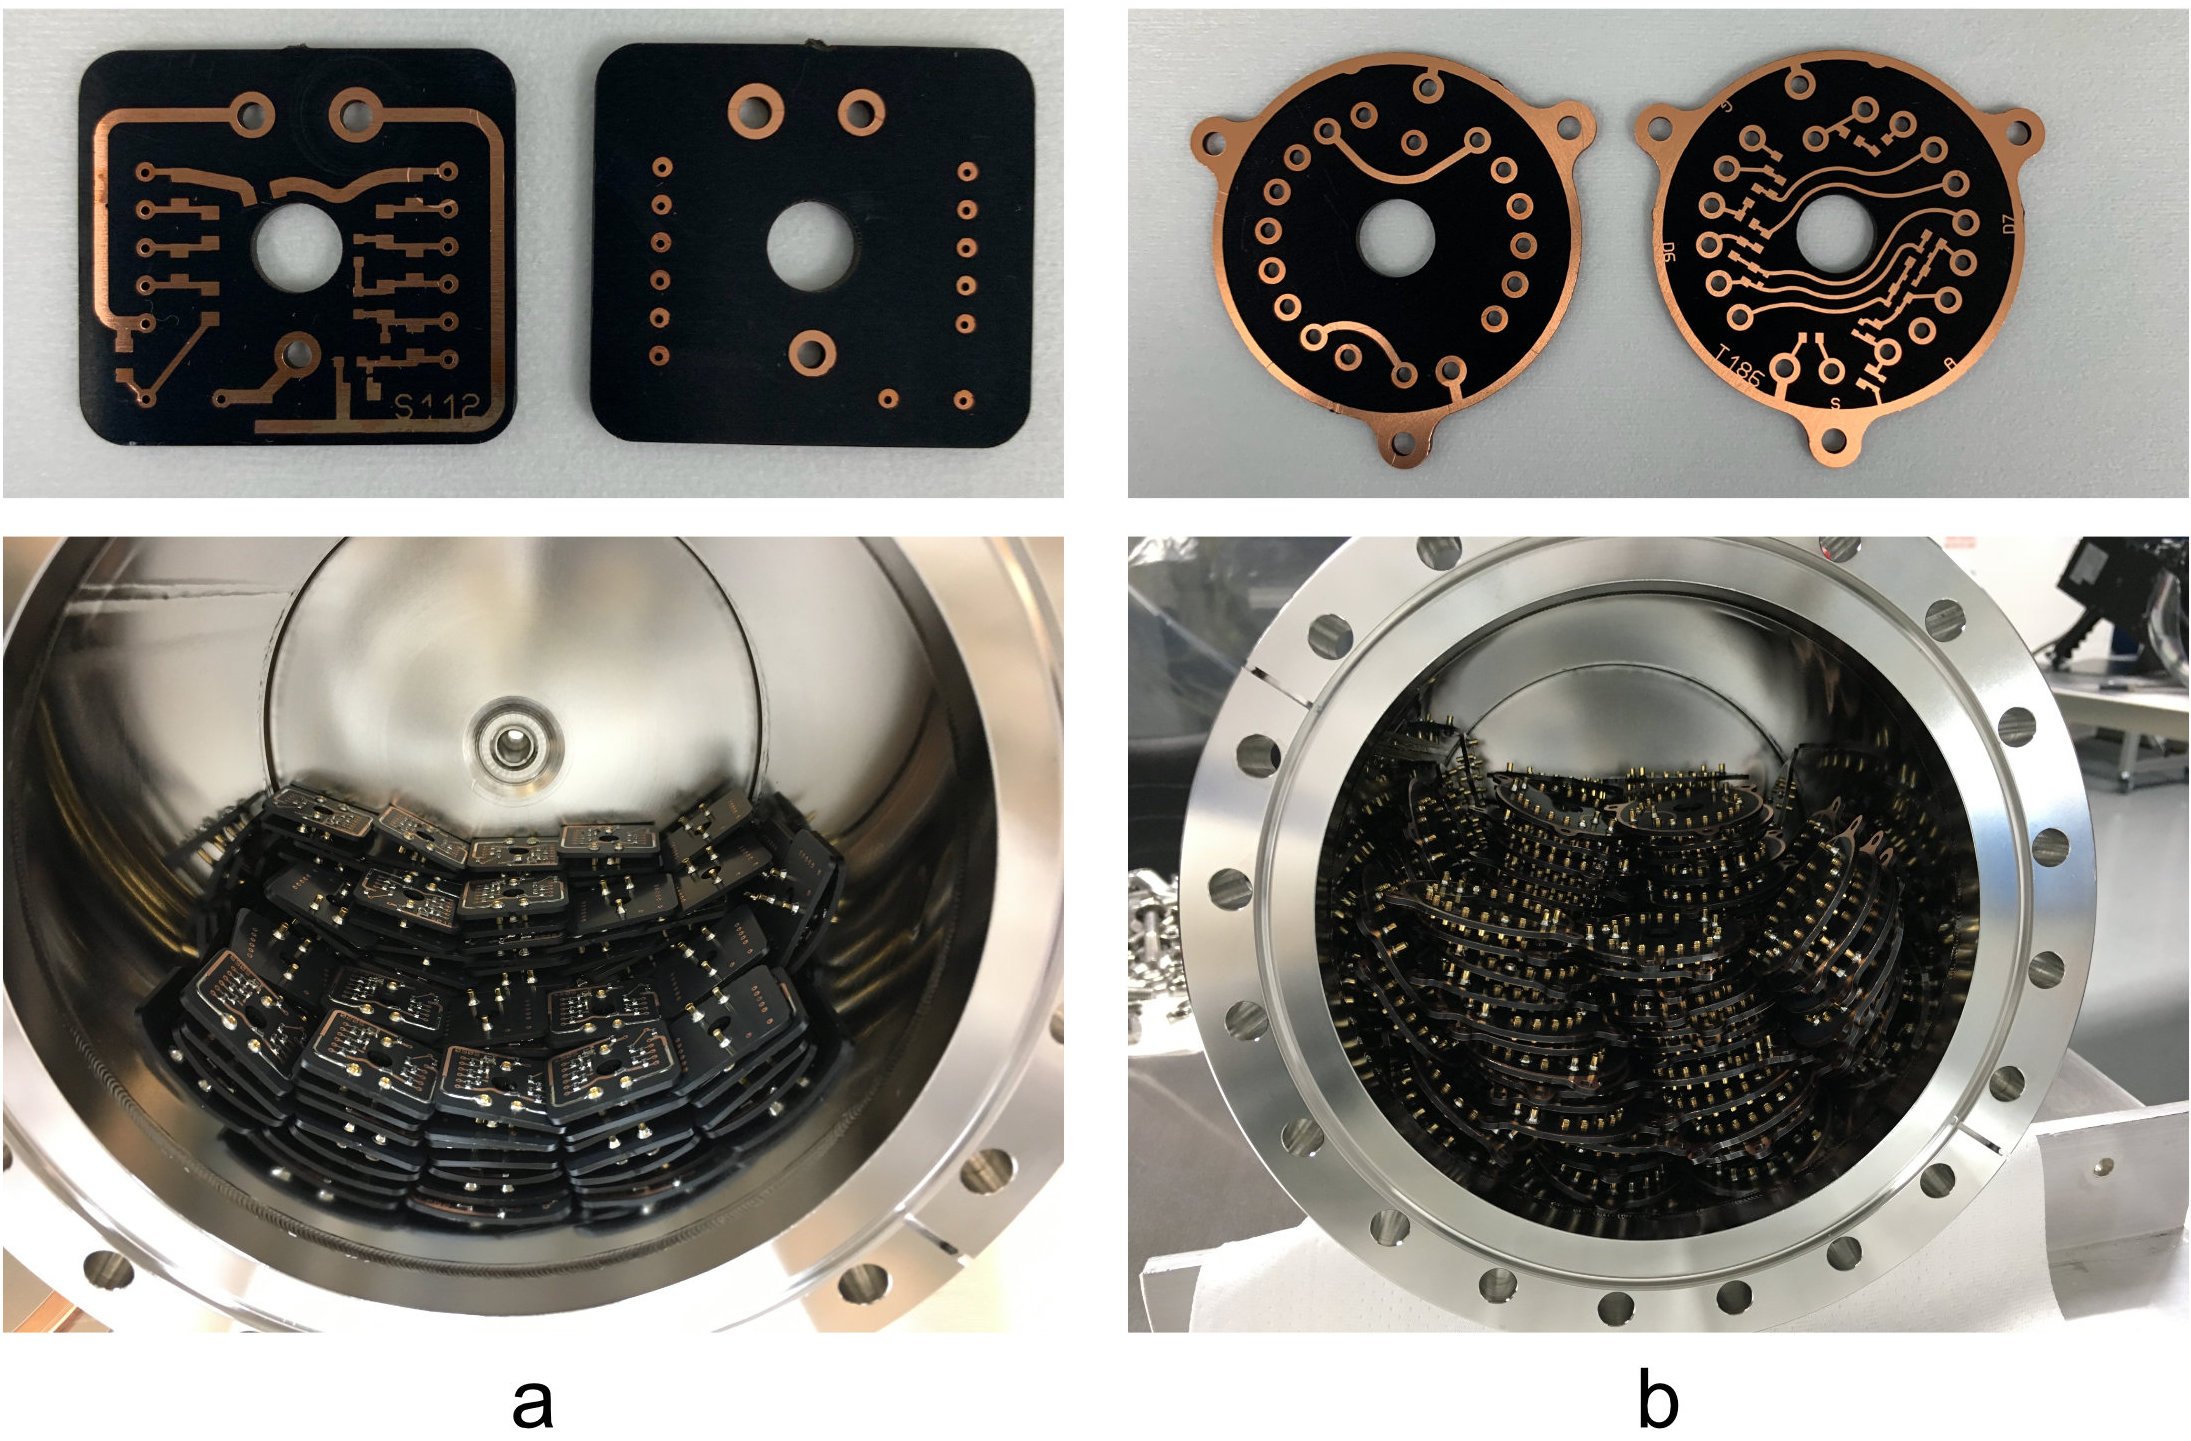
\includegraphics[scale=0.2]{Chapter_4/Figures/ucl_measurements/pmt_bases.jpg}
    \caption[A pictorial diagram of the 1" (a) and 3" (b) PMT base boards and their positioning within the UCL emsanation chamber.]
    {A pictorial diagram of the 1" (a) and 3" (b) PMT base boards and their positioning within the UCL emsanation chamber.}
    \label{fig:1_and_3_inch_bases}
\end{figure}
%
%
\begin{table}[h]
\centering
\caption{Relation of components in the different kind of LZ bases. The Cirlex mass is proportional to the Cirlex surface since all the bases are made of a 1.5 mm thick Cirlex PCB. All resistors and capacitors have the same dimensions. Regarding the solder, please refer to the text.}
\label{tab:pmt_base_components}
\vspace{1mm}
\renewcommand{\arraystretch}{1.2}
    \begin{tabularx}{.9\linewidth}{@{\extracolsep{\fill}}llll}
    \toprule
    
    \textbf{Components} & %1
    \textbf{3" PMT Bases} & %2
    \textbf{2" PMT Bases} & %3
    \textbf{1" PMT Bases} & %4
    
    \hline
    \hline
    
    Cirlex PCB	    & 3300 mg       & 3300 mg       & 1680 mg   \\
    Resistors       & 15 units      & 15 units      & 13 units  \\       
    Capacitors	    & 5 units       & 5 units       & 3 units   \\        
    Receptacles	    & 19 units      & 20 units      & 3 units   \\       
    Solder  	    & 180 mg        & 180 mg        & 300 mg    \\       
    
    \bottomrule
    \end{tabularx}
\end{table}


%

Although the bases are all constructed from the same material, they do differ in the quantity of components use. These differences are highlighted in table \ref{tab:pmt_base_components}. The 3" and 2" PMT bases are essentially identical in size and component use, with the only minor difference being the additional receptacle used on the 2" PMT base. Hence, the results obtained for 3" bases are also assumed for 2" bases. The 1" bases are substantially different and hence were separately screened. The 180 mg value quoted for the total mass of solder used per 3" base was measured by weighing the bases before and after solder was applied. However, the same approach was not conducted for the 1" bases. The difficulty in doing a similar measurement was due to the variation in the amount of solder used for an individual 1" base. The 1" bases use similar number of components and in addition to this, they contain two reinforced solder tracks, hence a 300 mg was adopted as a best estimate. 


\subsubsection{Emanation of 3" Bases}

A total of 124 3" bases were packaged inside radon tight bags at the Imperial College cleanroom and transported to the radon facility cleanroom at UCL. Each base was then carefully taken out of the radon tight packaging and placed inside the emanation chamber with caution to avoid scratching or damaging base components. After the emanation period, the radon was transferred into the electrostatic detector and measurements on the decay rates of \PoTOF{} and \PoTOE{} were made. A second measurement was followed before the bases were transported back to Imperial College. The pre-corrected \PoTOF{} rates from these two measurements are shown in figure \ref{fig:3_inch_pmt_base_results}. Although not provided, the \PoTOE{} rates were checked for completeness and was found to agree within error with those obtained from \PoTOF{}. The output from the \PoTOF{} result was then corrected by applying the detector efficiency corrections detailed in section \ref{sec:detector_efficiency} to give a total radon emanation rate of $0.62\pm0.11$ mBq and $0.70\pm0.11$ mBq for 124 3" bases for the first and the second measurement respectively. 
%
\begin{figure}[h!]
    \centering
    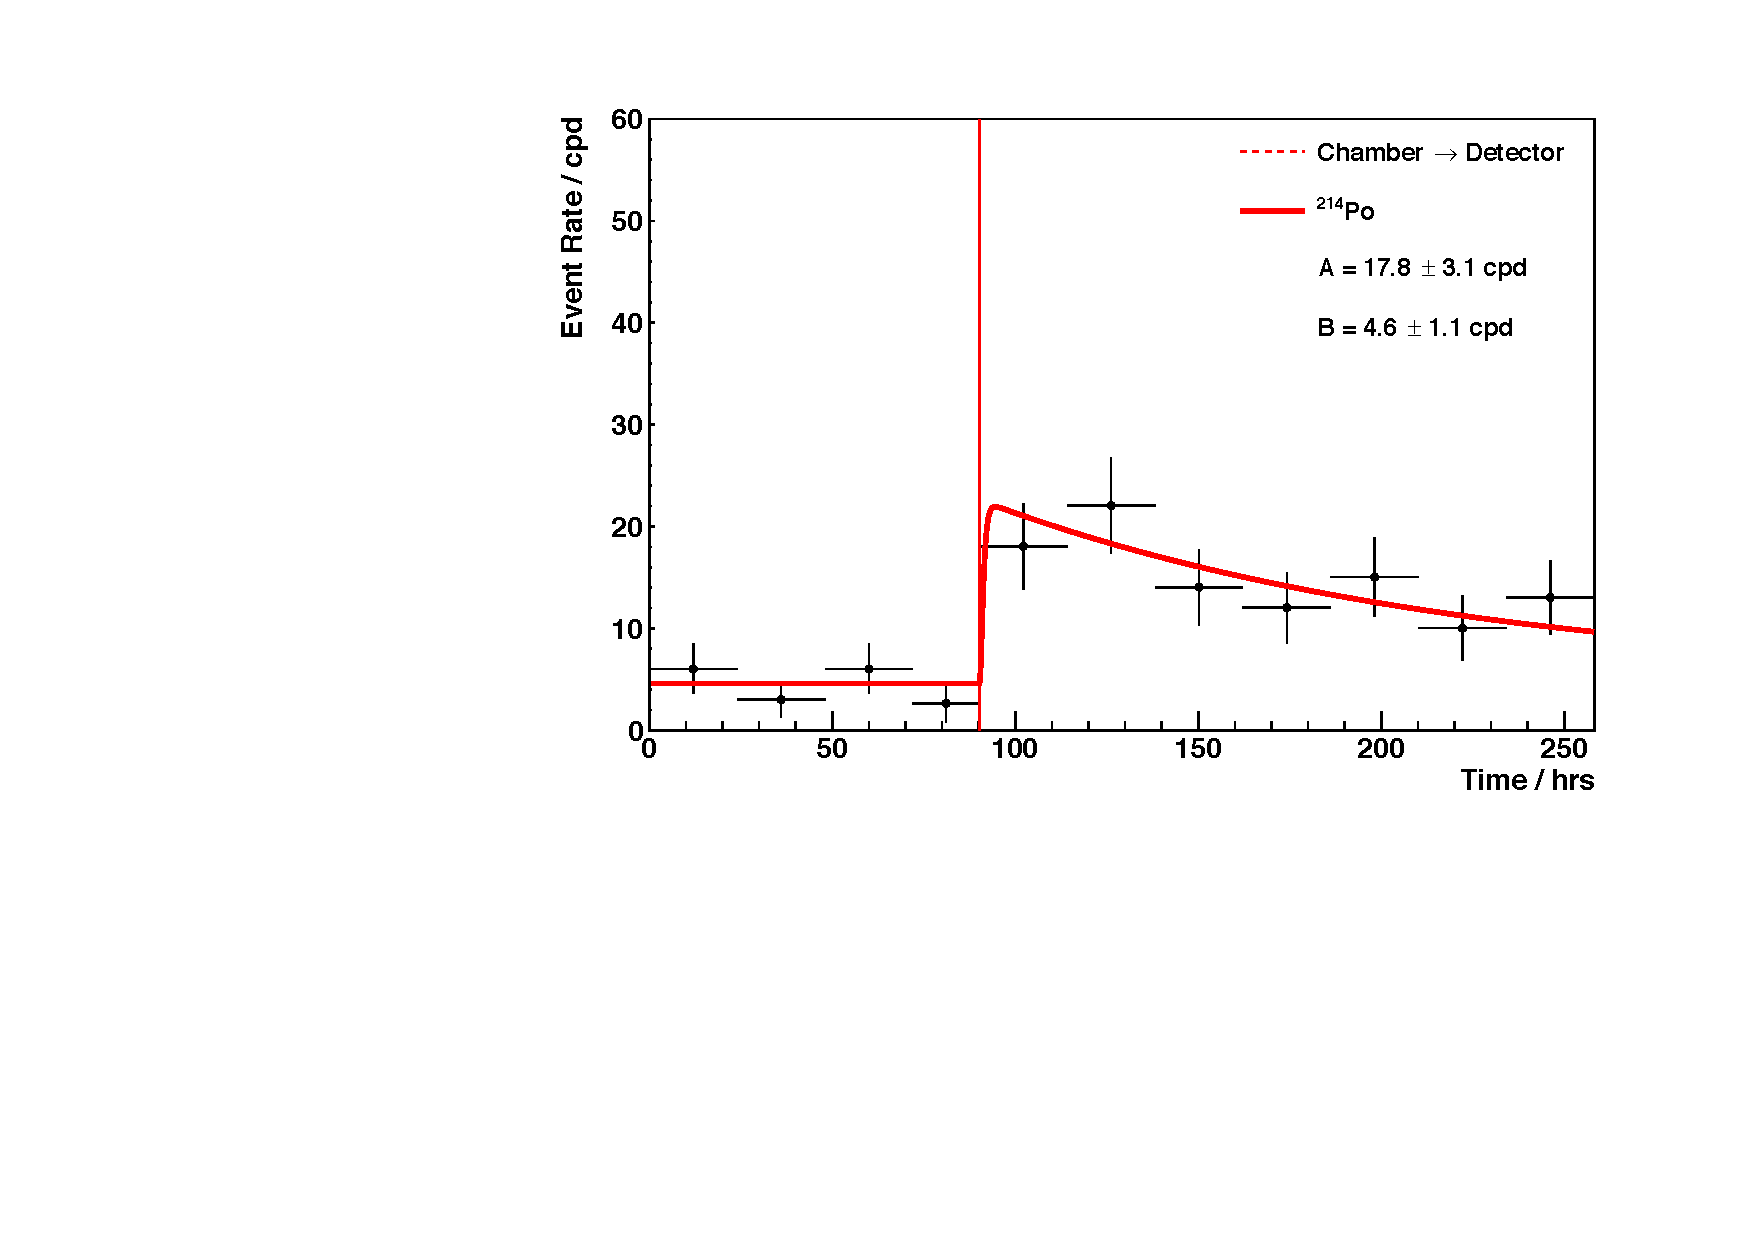
\includegraphics[scale=0.42]{Chapter_4/Figures/ucl_measurements/3_inch_bases_first_Po214.pdf}
    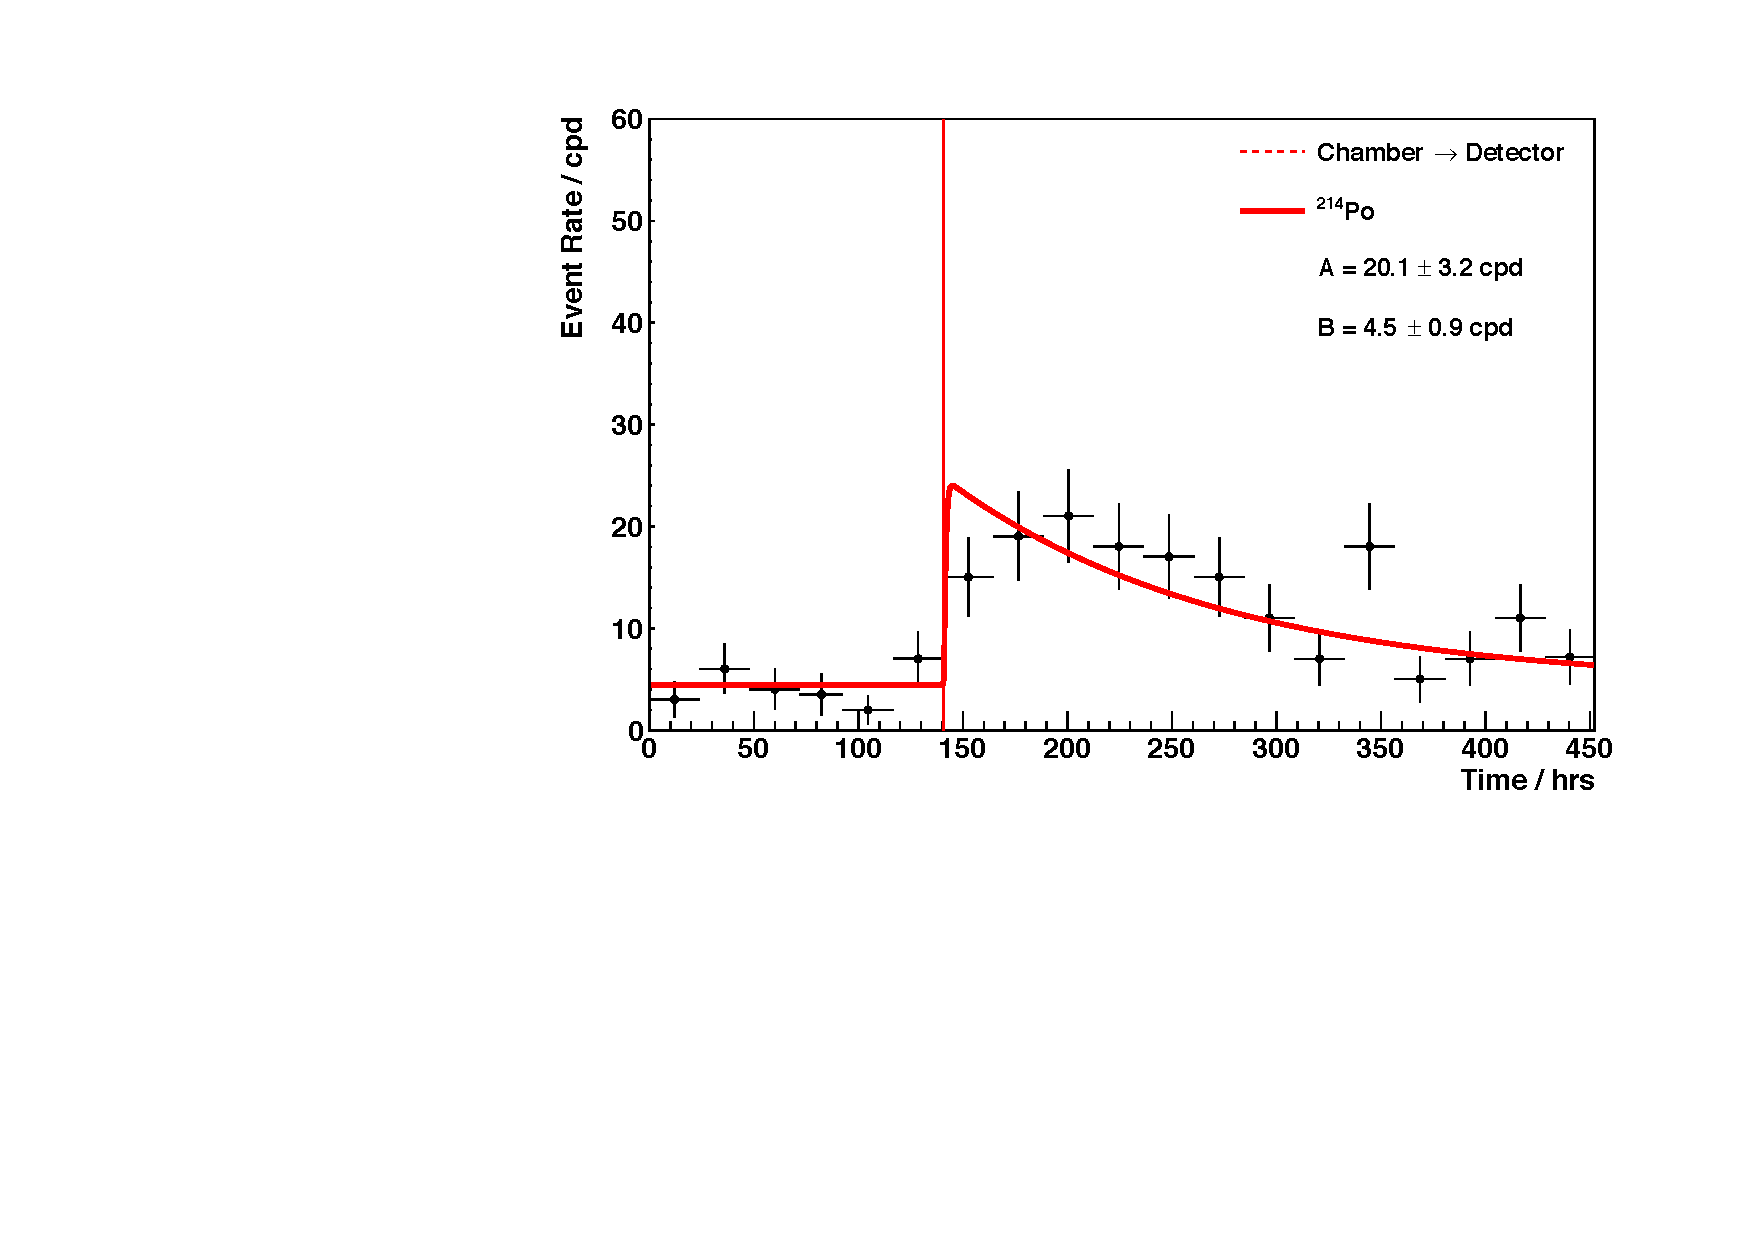
\includegraphics[scale=0.42]{Chapter_4/Figures/ucl_measurements/3_inch_bases_second_Po214.pdf}
    \caption[Pre-corrected \PoTOF{} event rate results obtained from the two measurements made on the 124 3" PMT bases screened using the UCL radon emanation system.]
    {Pre-corrected \PoTOF{} event rates of 124 3" PMT bases screened using the UCL radon emanation system. The bases were prepared and cleaned with a procedure identical to those used in the LZ detector.}
    \label{fig:3_inch_pmt_base_results}
\end{figure}
%


\subsubsection{Emanation of 1" Bases}

The emanation results from the 3" bases yielded a large discrepancy between the bottom-up estimations, hence 120 1" bases were emanated at the UCL facility to determine the radon background from these bases, as the bottom-up estimations were no longer reliable for the LZ background projections. Furthermore, the instrumental differences between the 3" and 1" could help understand why such a large discrepancy was observed; whether some of the components making up the bases were more radioactive than expected. These bases were treated identically to the 3" bases; initially cleaned at the Imperial College cleanroom to remove any surface contamination, and later transported to the UCL facility in radon tight packaging to minimise radon plate-out. The pre-corrected results obtained for \PoTOF{} and \PoTOE{} rates are in agreement within error and their rates within the detector are shown in figure \ref{fig:1_inch_pmt_base_result}. The output from the \PoTOF{} decay rate is then corrected by applying the detector efficiency corrections and the radon emanation rate of 120 1" bases are calculated to be $0.53\pm0.11$ mBq. 
%
\begin{figure}[h!]
    \centering
    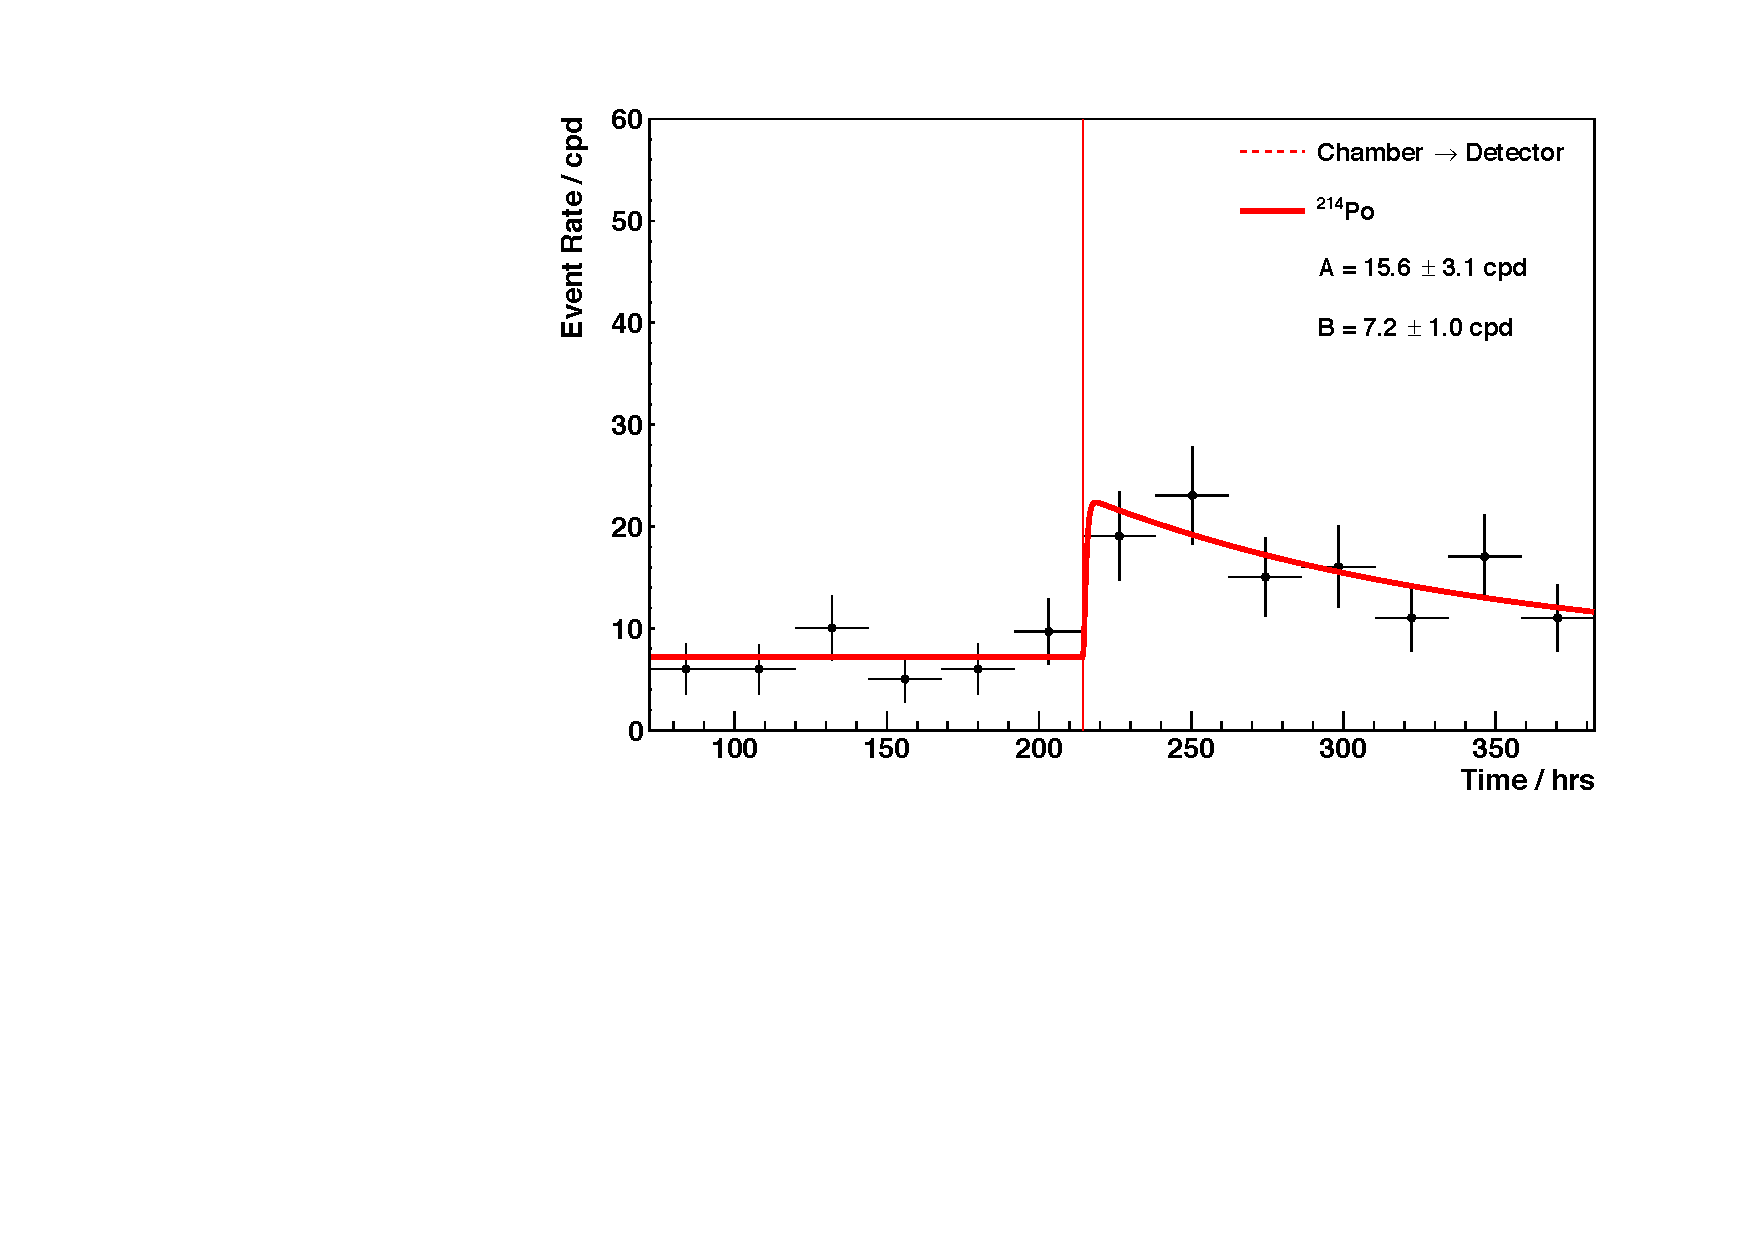
\includegraphics[scale=0.42]{Chapter_4/Figures/ucl_measurements/1_inch_base_Po214.pdf}
    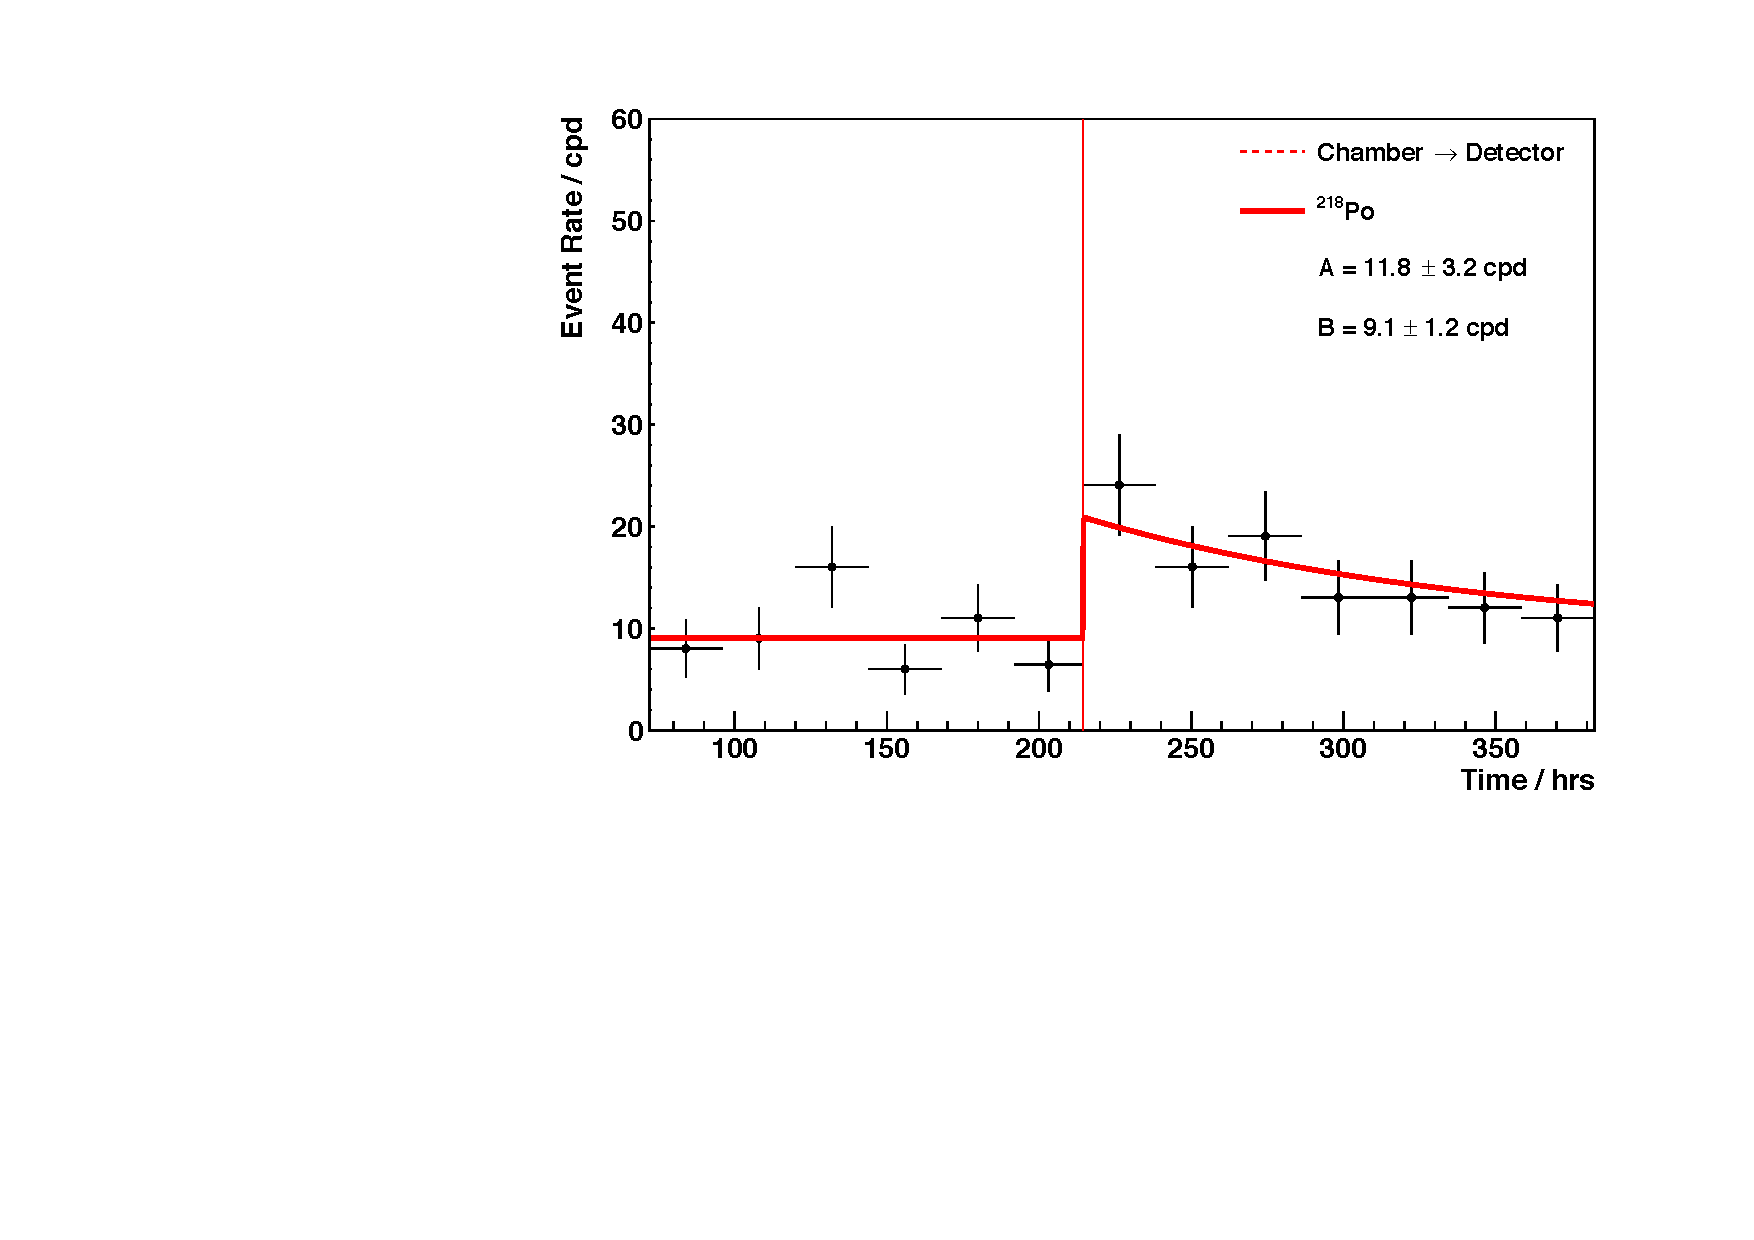
\includegraphics[scale=0.42]{Chapter_4/Figures/ucl_measurements/1_inch_bases_Po218.pdf}
    \caption[Pre-corrected \PoTOF{} (left) and \PoTOE{} (right) event rates of 120 1" PMT bases screening, representative of those that are used in LZ.]
    {Pre-corrected \PoTOF{} (left) and \PoTOE{} (right) event rates of 120 1" PMT bases screened using the UCL radon emanation system. The bases were prepared and cleaned with a procedure identical to those used in the LZ detector.}
    \label{fig:1_inch_pmt_base_result}
\end{figure}
%


\subsubsection{Discussion \& Conclusion}

%
\begin{table}[b]
\centering
\caption
[HPGe screening of rock, shotcrete and gravel samples from the Davis cavern laboratory.]
{Radon emanation results as obtained from the UCL system for the 3" and the 1" bases with bottom-up comparisons. All the results are given per respective base. A measurement from the XENON1T collaboration for 3" bases with almost identical design and component usage is provided for comparison \cite{Natascha}.}
\label{tab:pmt_base_results}
\vspace{1mm}
\renewcommand{\arraystretch}{1.2}
    \begin{tabularx}{.9\linewidth}{@{\extracolsep{\fill}}lll}
    \toprule
    
    \textbf{Measurement} & %1
    \textbf{3" Bases [\micro{}Bq/base]} & %2
    \textbf{1" Bases [\micro{}Bq/base]} & %3
    
    \hline
    \hline
    
    Bottom-up 	            & 1.65\pm0.56$      & 1.25\pm0.47       \\
    1$^{st}$ Measurement    & $5.00\pm0.86$     & $4.42\pm0.90$     \\       
    2$^{nd}$ Measurement	& $5.65\pm0.90$     & -                 \\        
    \hline
    Averaged	            & $5.33\pm0.63$     & $4.42\pm0.90$     \\       
    XENON1T Bases           & $3.0\pm0.6$       & - \\
    
    \bottomrule
    \end{tabularx}
\end{table}


%
The radon emanation results from the 3" and the 1" bases, along with their bottom-up estimates are highlighted in table \ref{tab:pmt_base_results} for comparison. The results indicate a radon emanation activity of 5.33 \micro{}Bq and 4.42 \micro{}Bq per 3" and 1" base; which is 3.68 \micro{}Bq and 3.17 \micro{}Bq above the bottom-up estimation respectively. Although the 1" bases have less Cirlex and electronic components, the activity in comparison to the 3" bases are relatively high, suggesting the solder to have a non-zero activity comparable to some of the components taken into account. In assuming the 3" bases emanation rate also applied to the 2" bases, the contributions from all LZ bases together returns a total contribution of $3.21 \pm 0.35$ mBq.  Furthermore, a cross-calibration campaign between all of the radon facilities used by LZ, as highlighted in section \ref{sec:otherradon}, indicated an upwards systematic for the UCL radon emanation system of 1.53 when compared to the base rate of the sample. In considering this systematic, the total radon emanation rate of the bases go down to $2.10\pm0.23$ mBq. This equates to an activity of $3.38\pm0.41$ \micro{}Bq/[3” base]---in good agreement with the result obtained by XENON1T \cite{Natascha}. It is important to note that these values do not assume any reduction in rate due to temperature and the actual rate in LZ may be lower due a temperature suppression.


\subsection{Cryostat Titanium \& Titanium Welding}
\label{secsec:titanium_emanation}

In the early stages of the LZ experiment, an extensive R\&D campaign was conducted to source and produce enough titanium for the cryostat vessels of the detector. The ICV and the OCV, which contain the TPC and the 10 tonnes of LXe, make up a significant bulk of the LZ detector. Due to their scale and proximity to the TPC, it was necessary to ensure ultra-low levels of radiopurity for \UTTE{} and \ThTTT{} isotopes as well as \KFZ{} and \CoSZ{}. A detailed analysis using ICP-MS and gamma-ray spectroscopy of 22 different titanium samples was conducted, and the sample of the HN3469 product manufactured by TIMET was found to have the lowest background. The measured activities for \UTTEe{}, \ThTTTe{}, \CoSZ{} and \KFZ{} from the sample are significantly lower than requirements and were the lowest reported to date \cite{LZ_titanium_selection}. 

Assuming chemical equilibrium within the titanium for both the uranium and thorium series, the ultra-low activities measured by the ICP-MS facility for \UTTEe{} (<0.13 ppb) and \ThTTTe{} (0.069(7) ppb) lead to a negligible amount of radon emanation, with the assumption that diffusion would be heavily suppressed due to the dense metallic nature of titanium. To this day, there are no known measurement of radon emanation from titanium, however, results from steel sheets and welding have previous been reported by the GERDA collaboration with activities in $\mathcal{O}(10)$ \uBqms \cite{osti_20719228, ZUZEL2009889}. 

Although the OCV is relevant for \grays, backgrounds for radon emanation is only expected from the ICV and its inner content. The ICV uses a total of 950 kg of titanium with several other titanium pieces used for structural support of PMTs, both in the skin region and within the TPC. Furthermore, the ICV is made up of several smaller segments welded together using $\sim$6 kg of titanium welding rods. After the installation of the skin region at SURF, the ICV was sealed and left to emanate. The results obtained from the harvested radon from the ICV indicated an emanation rate of $28.3\pm2.0$ mBq; in comparison to this, the expected bottom-up emanation from individual measurements of components within the ICV was only $2.3^{+3.7}_{-0.9}$ mBq. This large discrepancy was unexpected and prompted a radon screening campaign to examine some of the potential sources; emanation from dust accumulation and from unaccounted components (i.e. titanium cryostat and welding). 

To examine radon emanation from the welded surface and the raw titanium surface, a 7 mm titanium plate welded with titanium and several titanium cutouts from the OCV were shipped to the UCL radon facility. A pictorial diagram of these two samples can be seen in figure \ref{fig:titanium_welding_sheets} just before their respective emanation periods. The welded block was originally constructed from the LZ stock to study abnormally high ICP-MS measurements, detailed in \cite{lz_screening}.
%
\begin{figure}[t]
    \centering
    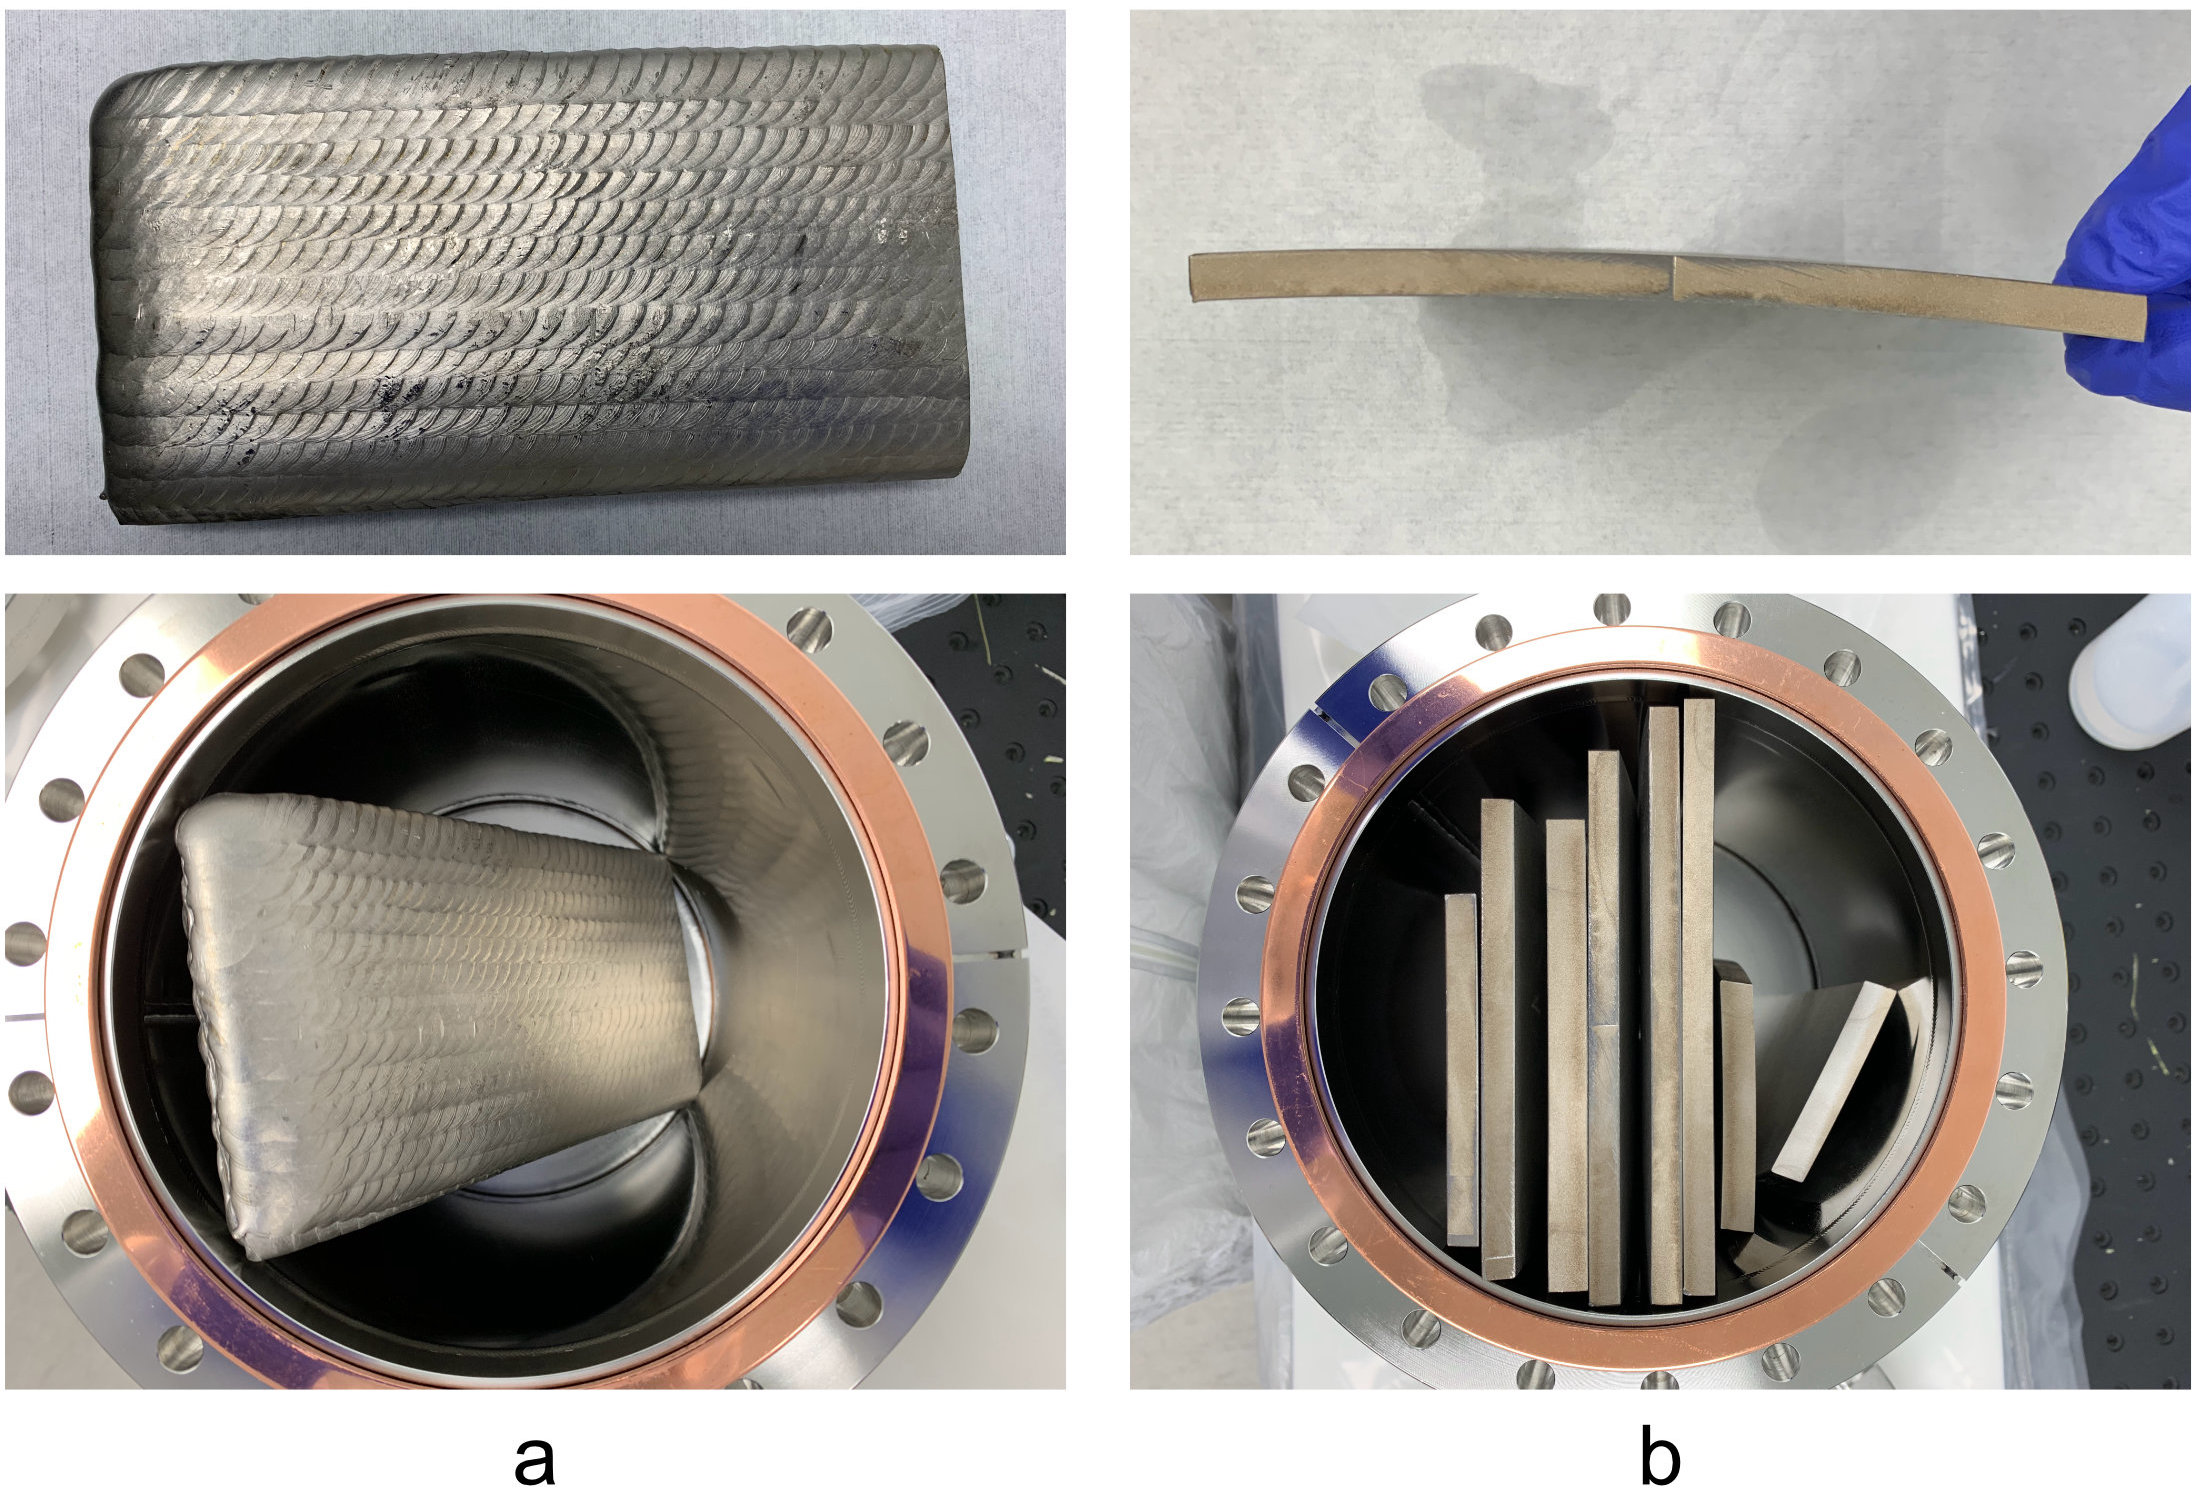
\includegraphics[scale=0.2]{Chapter_4/Figures/ucl_measurements/titanium_and_welding.jpg}
    \caption[A pictorial diagram of welded titanium block and the titanium sheets cut-off from the LZ OCV.]
    {A pictorial diagram of welded titanium block (a) and the titanium sheets (b) cut-off from the LZ OCV.}
    \label{fig:titanium_welding_sheets}
\end{figure}
%


\subsubsection{Titanium Welding}

To examine radon emanation from a titanium welded surface, a sample of 7 mm Ti plate with a large TIG weld on both sides with a total welding surface area of 325 cm\squared{} was assayed at the UCL facility. The sample is one of four blocks originally prepared for quality control during the ICV and OCV manufacturing. Studies on this sample using ICP-MS yielded concentration of $0.16\pm0.04$ ppb \UTTEe{} and $3.20\pm0.16$ ppb \ThTTTe{}. The higher levels of \ThTTTe{} were attributed to the inadvertent use of thoriated electrodes, which was later corrected as a result of this study with no impact on background. The final welding used inside the ICV was from the same titanium stock but used lanthanated elecrodes. \RnTTT{} is strictly coming from the \UTTE{} decay chain and hence the results highlighted here are assumed to apply to lanthanated welding. Two sets of measurements were performed on the welded block: emanation prior to etching and post etching by AstroPak---a certified professional precision cleaning company. Results obtained for the pre-etched and post-etched block are shown in figure \ref{fig:ti_pre_etched_welded_block_results} and \ref{fig:ti_post_etched_welded_block_results}, respectively. Pre-etched block was measured once, whereas the post-etched block was measured twice.
%
\begin{figure}[h!]
    \centering
    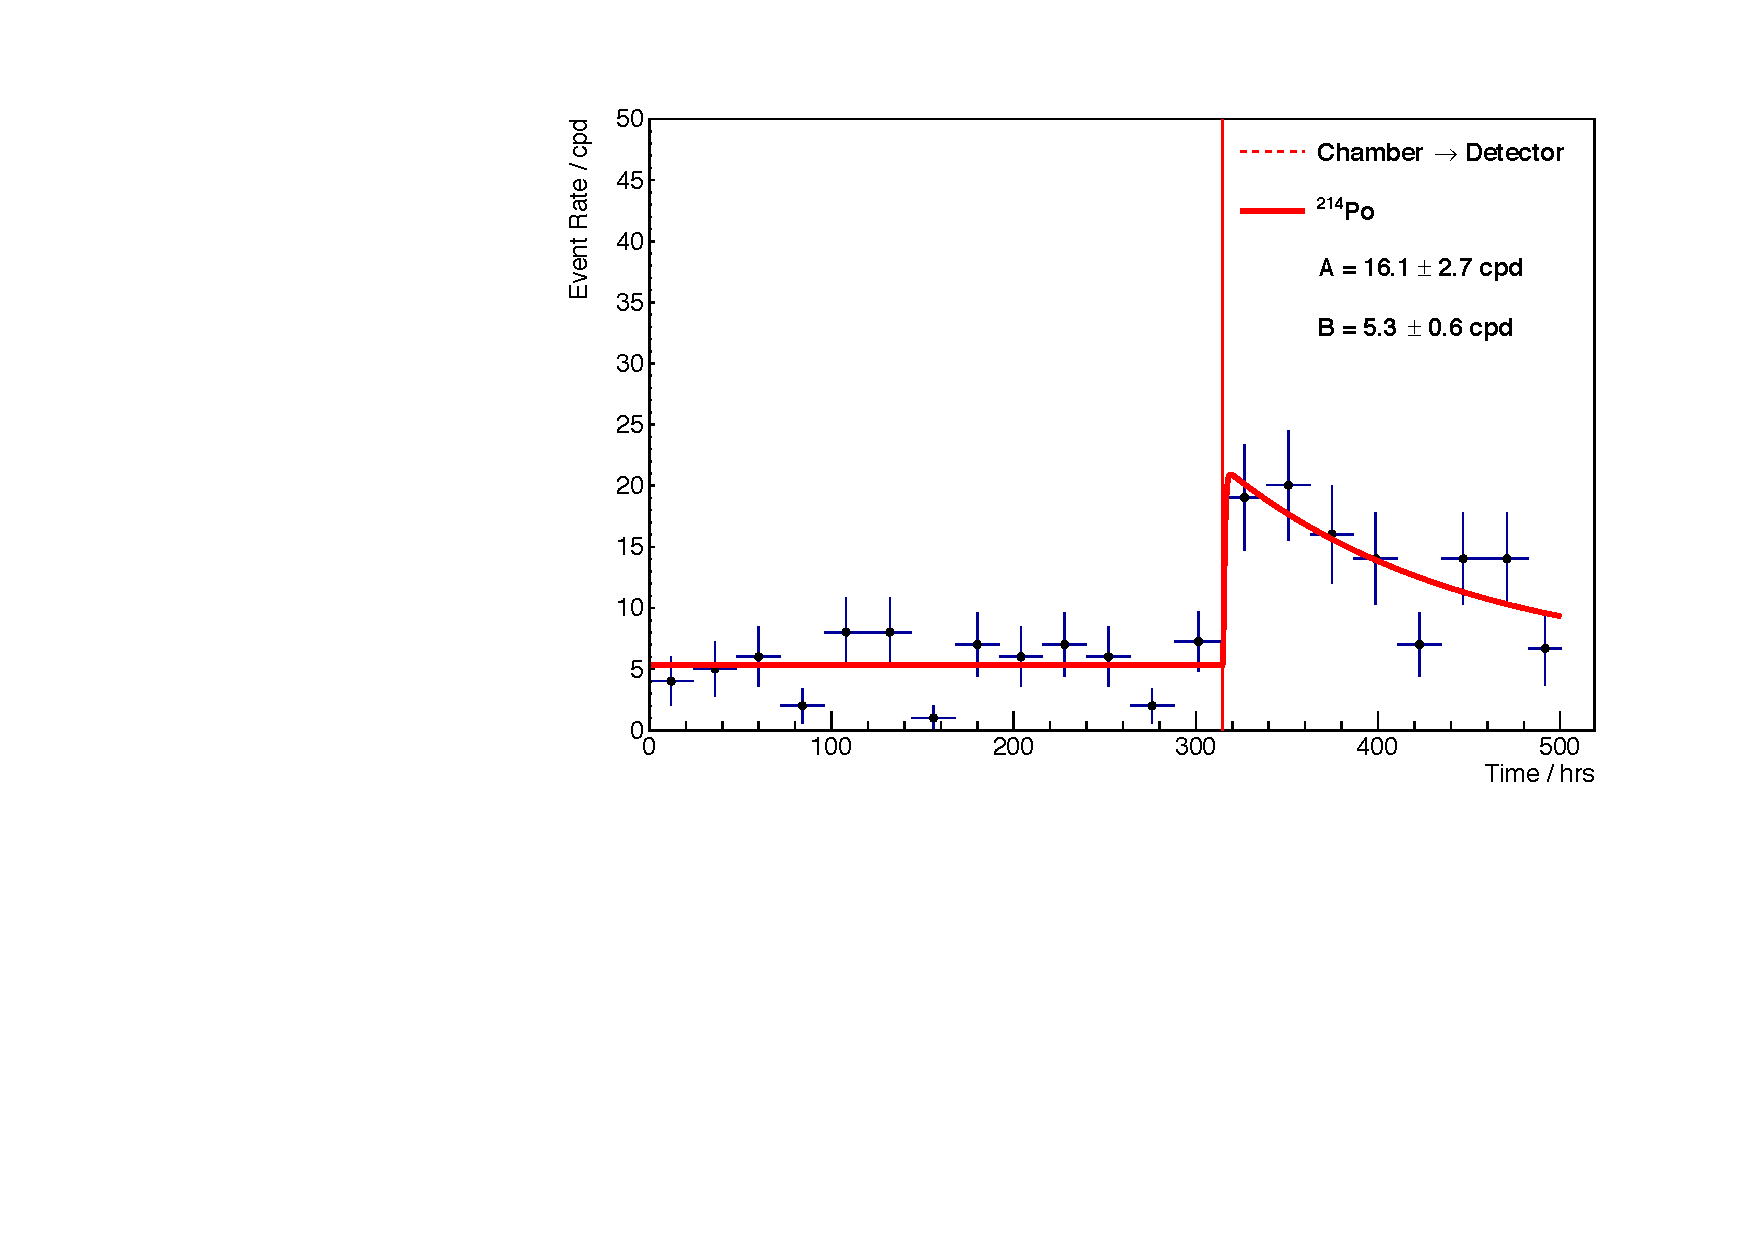
\includegraphics[scale=0.42]{Chapter_4/Figures/ucl_measurements/titanium_welding_block_pre_etching_1_Po214.pdf}
    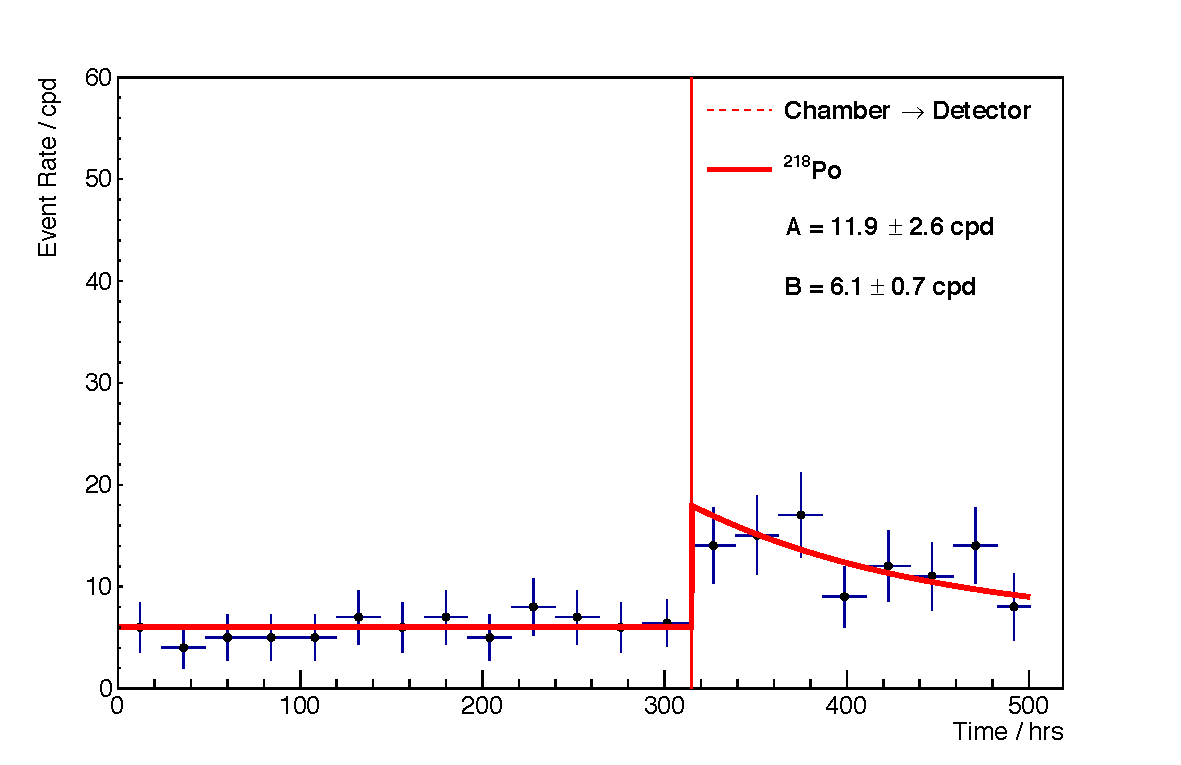
\includegraphics[scale=0.42]{Chapter_4/Figures/ucl_measurements/titanium_welding_block_pre_etching_1_Po218.pdf}
    \caption[Pre-corrected \PoTOF{} and \PoTOE{} event rate results obtained from the single measurement made on the pre-etched titanium welded block.]
    {Pre-corrected \PoTOF{} and \PoTOE{} event rate results obtained from the single measurement made on the pre-etched titanium welded block. The block was initially wiped extensively with wet cleanroom wipes and ultrasonic bathed.}
    \label{fig:ti_pre_etched_welded_block_results}
\end{figure}
%
%
\begin{figure}[h!]
    \centering
    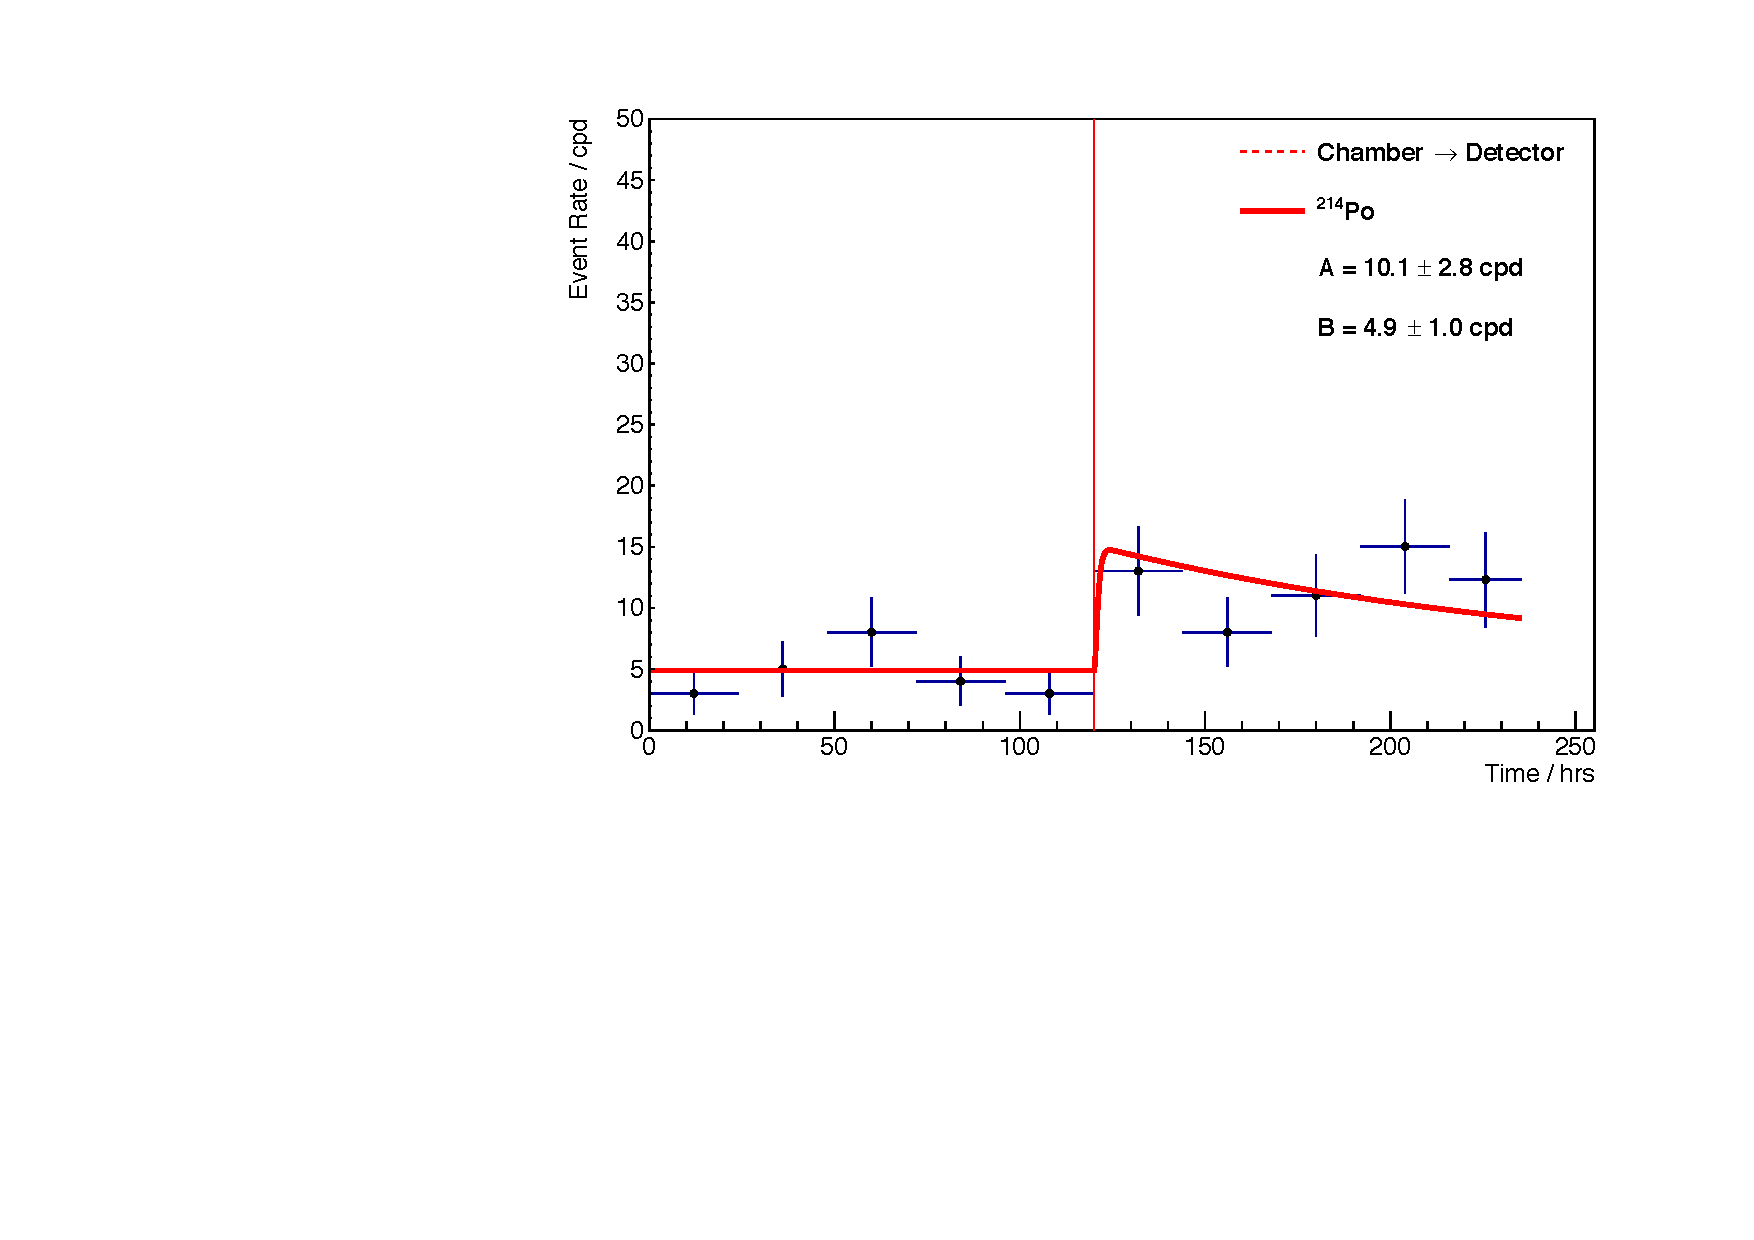
\includegraphics[scale=0.42]{Chapter_4/Figures/ucl_measurements/titanium_welding_block_post_etching_1_Po214.pdf}
    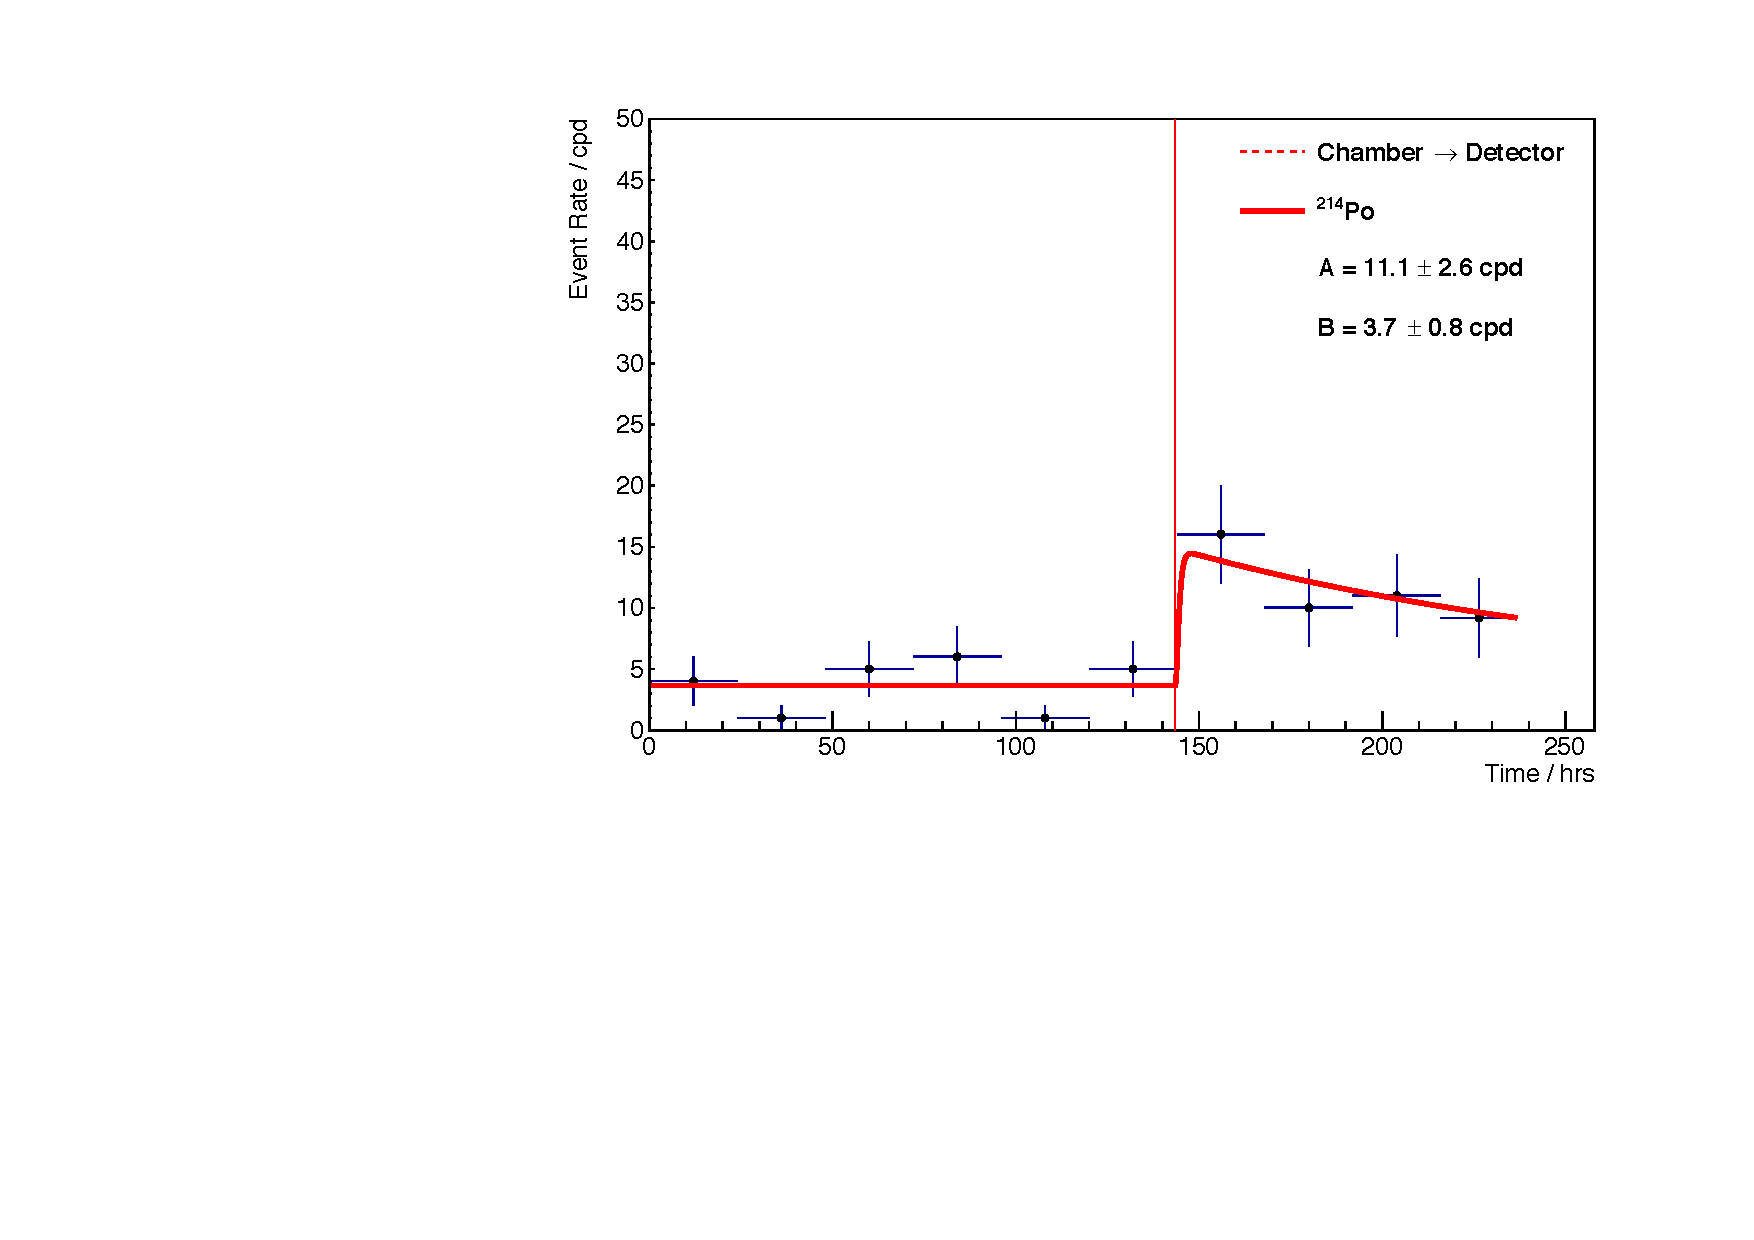
\includegraphics[scale=0.42]{Chapter_4/Figures/ucl_measurements/titanium_welding_block_post_etching_2_Po214.pdf}
    \caption[Pre-corrected \PoTOF{} event rate results obtained from the two measurements made on the post-etched titanium welded block.]
    {Pre-corrected \PoTOF{} event rate results obtained from the two measurement made on the post-etched titanium welded block.}
    \label{fig:ti_post_etched_welded_block_results}
\end{figure}
%

The output from the \PoTOF{} rate of the pre-etched welded block indicated an emanation rate of $560\pm97$ \micro{}Bq, which was in good agreement with \PoTOE{} within error. The averaged output from the post-etched block indicated a rate of $370\pm68$ \micro{}Bq. Although the errors are relatively large and the dataset is constrained by so few measurements, the result seems to indicate that there is a substantial amount of radon emanating out of the block. 


\subsubsection{Titanium Sheets}

To examine radon emanation from the cryostat titanium, a collection of titanium cutouts from the OCV were assayed. 8 pieces totalling to an area of 2350 cm\squared{} were initially wiped down with cleanroom wipes and ultrasonic bathed to remove any dust residue. There sheets are identical to those used in the ICV. Two sets of measurements were performed on the sheets: pre-etched and post-etched measurements. The slight curvature on the sheets, as shown on figure \ref{fig:titanium_welding_sheets}, was used to minimise overlaps, which in theory could reduce emanation from recoil, as radon atoms from one surface can lodge into another surface. Results obtained for the pre-etched and post-etched sheets are shown in figure \ref{fig:ti_pre_etched_sheets_results} and \ref{fig:ti_post_etched_sheets_results}, respectively. Pre-etched block was measured once, whereas the post-etched block was measured three times.
%
\begin{figure}[b!]
    \centering
    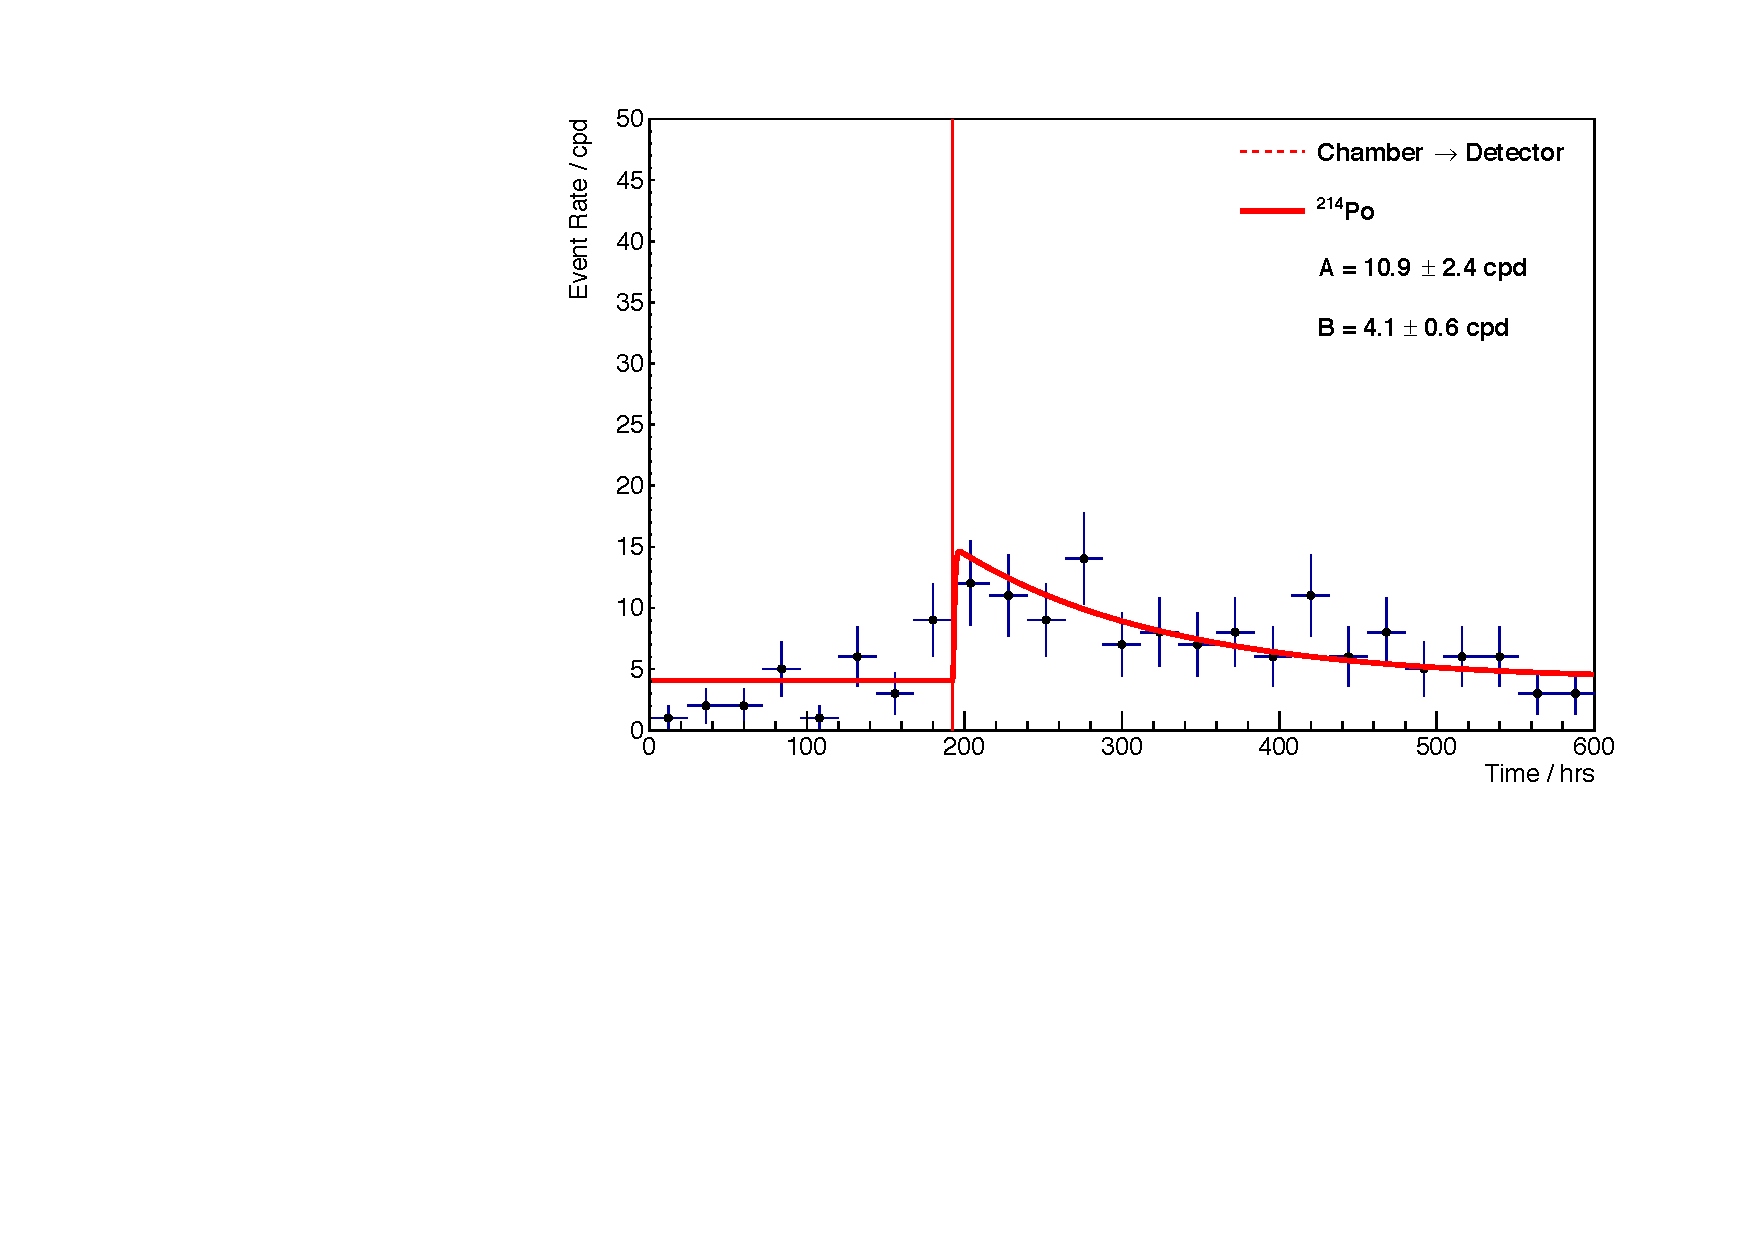
\includegraphics[scale=0.42]{Chapter_4/Figures/ucl_measurements/titanium_sheets_pre_etching_1_Po214.pdf}
    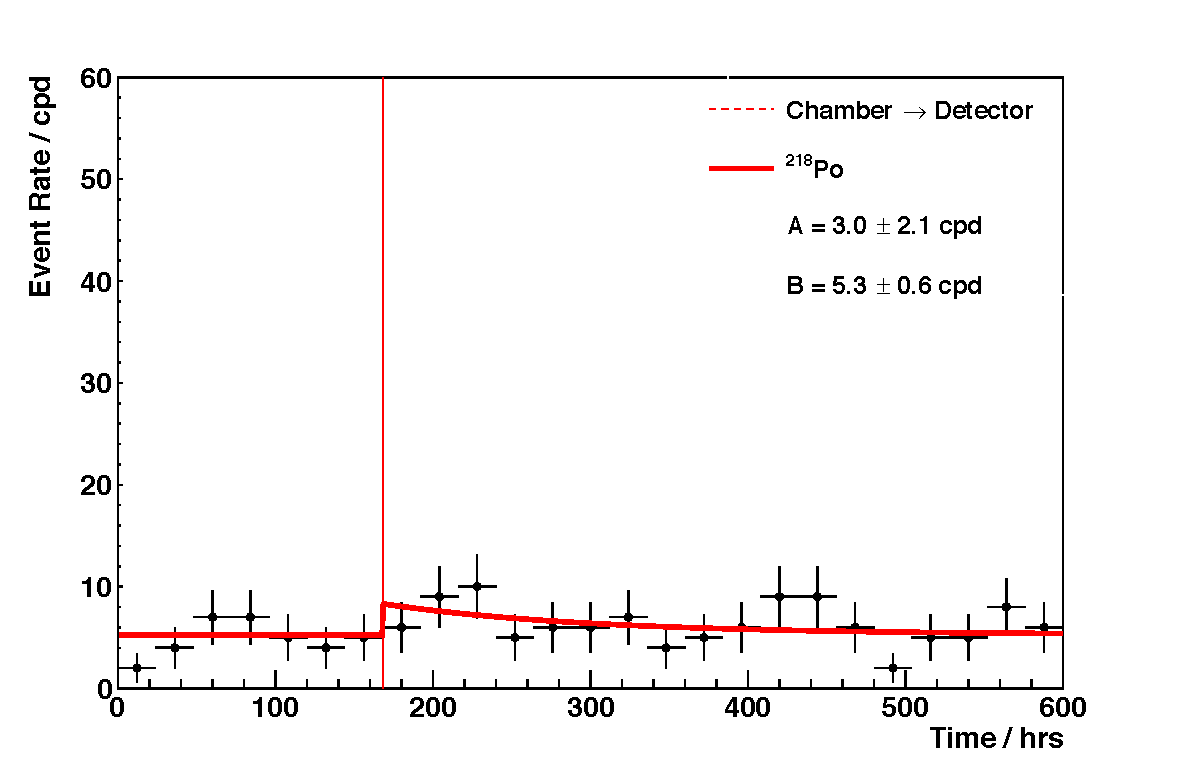
\includegraphics[scale=0.42]{Chapter_4/Figures/ucl_measurements/titanium_sheets_pre_etching_1_Po218.pdf}
    \caption[Pre-corrected \PoTOF{} and \PoTOE{} event rate results obtained from the single measurement made on the pre-etched titanium welded block.]
    {Pre-corrected \PoTOF{} and \PoTOE{} event rate results obtained from the single measurement made on the pre-etched titanium welded block.}
    \label{fig:ti_pre_etched_sheets_results}
\end{figure}
%

The output from the \PoTOF{} rate indicates an emanation rate above the background measured prior to transfer, corresponding to a corrected activity of $380\pm88$ \micro{}Bq. However, the \PoTOE{} rate suggests a background only measurement. This behaviour has previously been observed and is attributed to outgassing of certain samples, for example the \PoTOE{} in comparison to \PoTOF{} has been shown to be suppressed under the presence of (N$_{2}$O). Although a signal has been observed, the presence of neutralising agents may add a systematic error that's currently difficult to determine. 
%
\begin{figure}[t!]
    \centering
    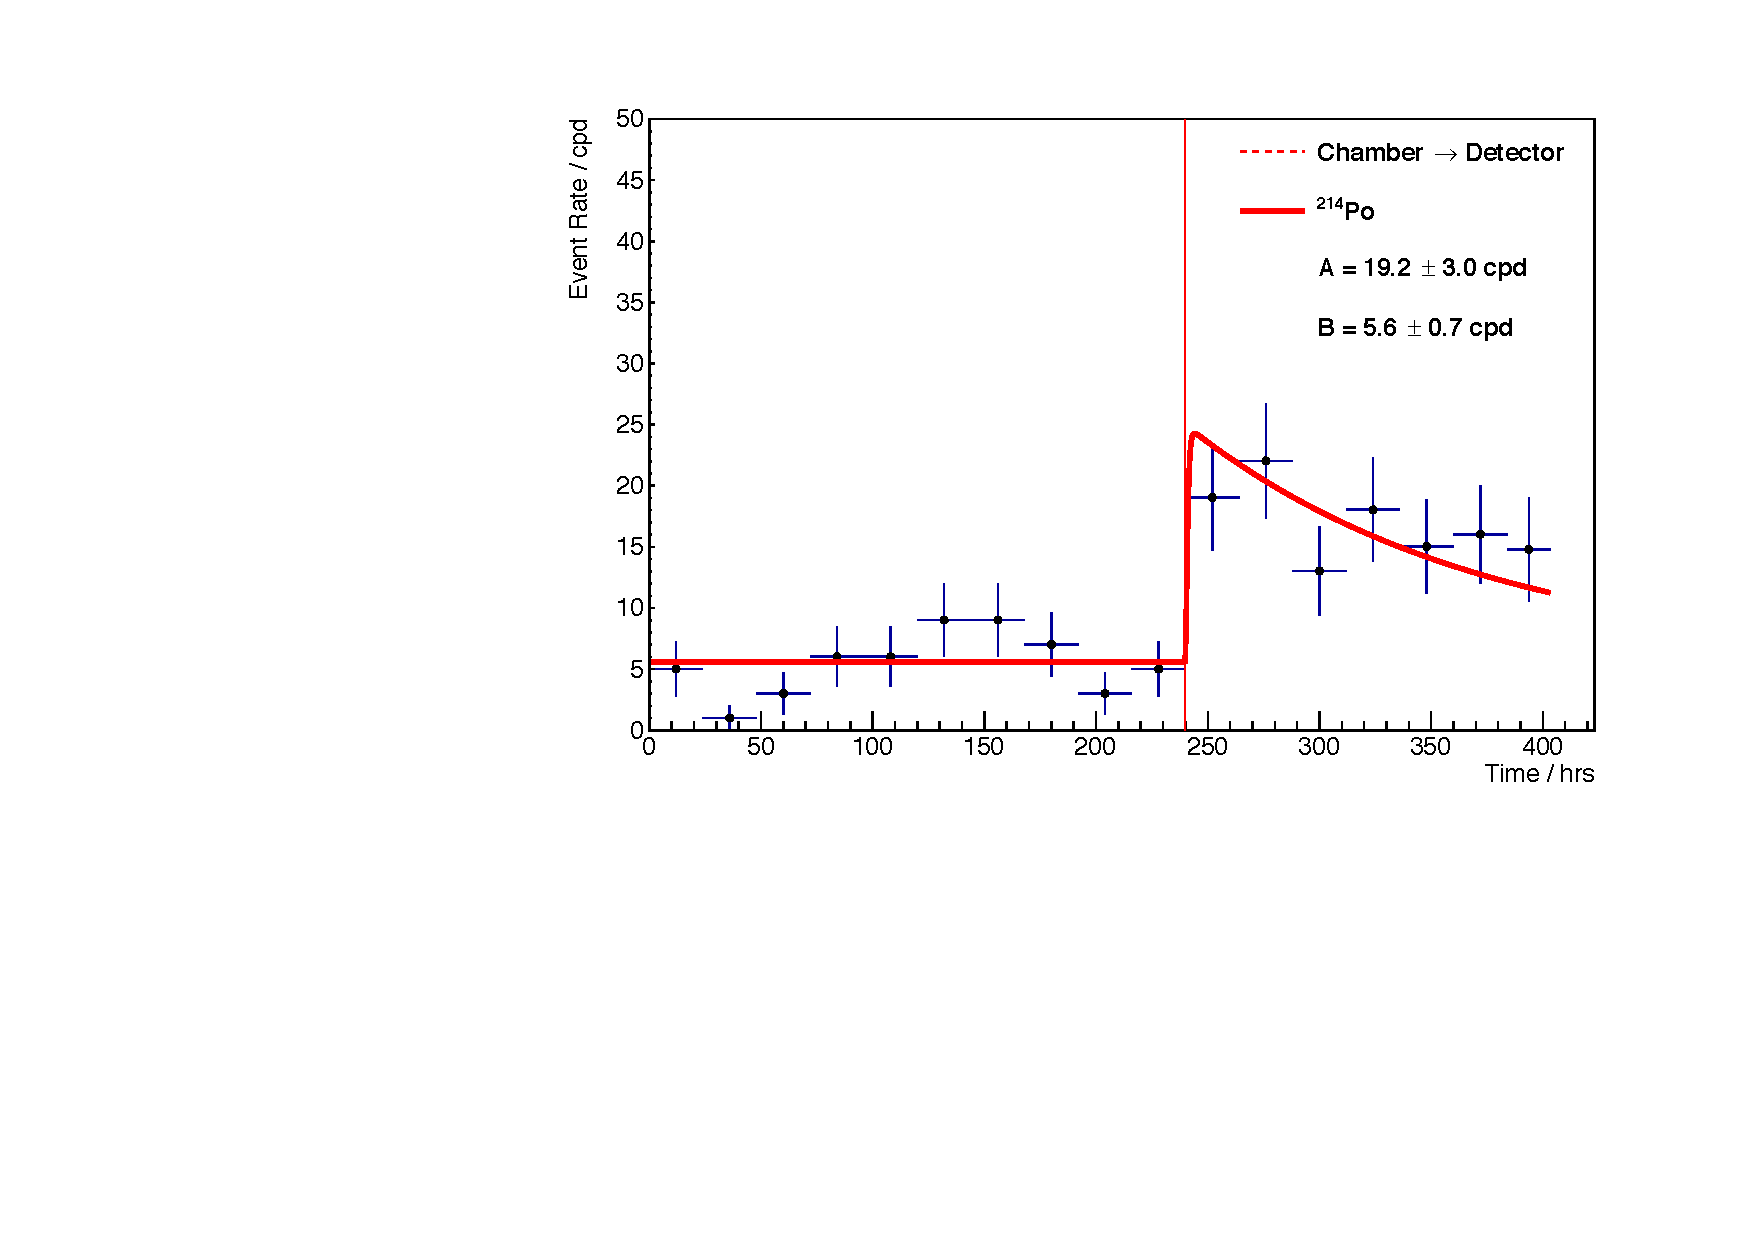
\includegraphics[scale=0.42]{Chapter_4/Figures/ucl_measurements/titanium_sheets_post_etching_1_Po214.pdf}
    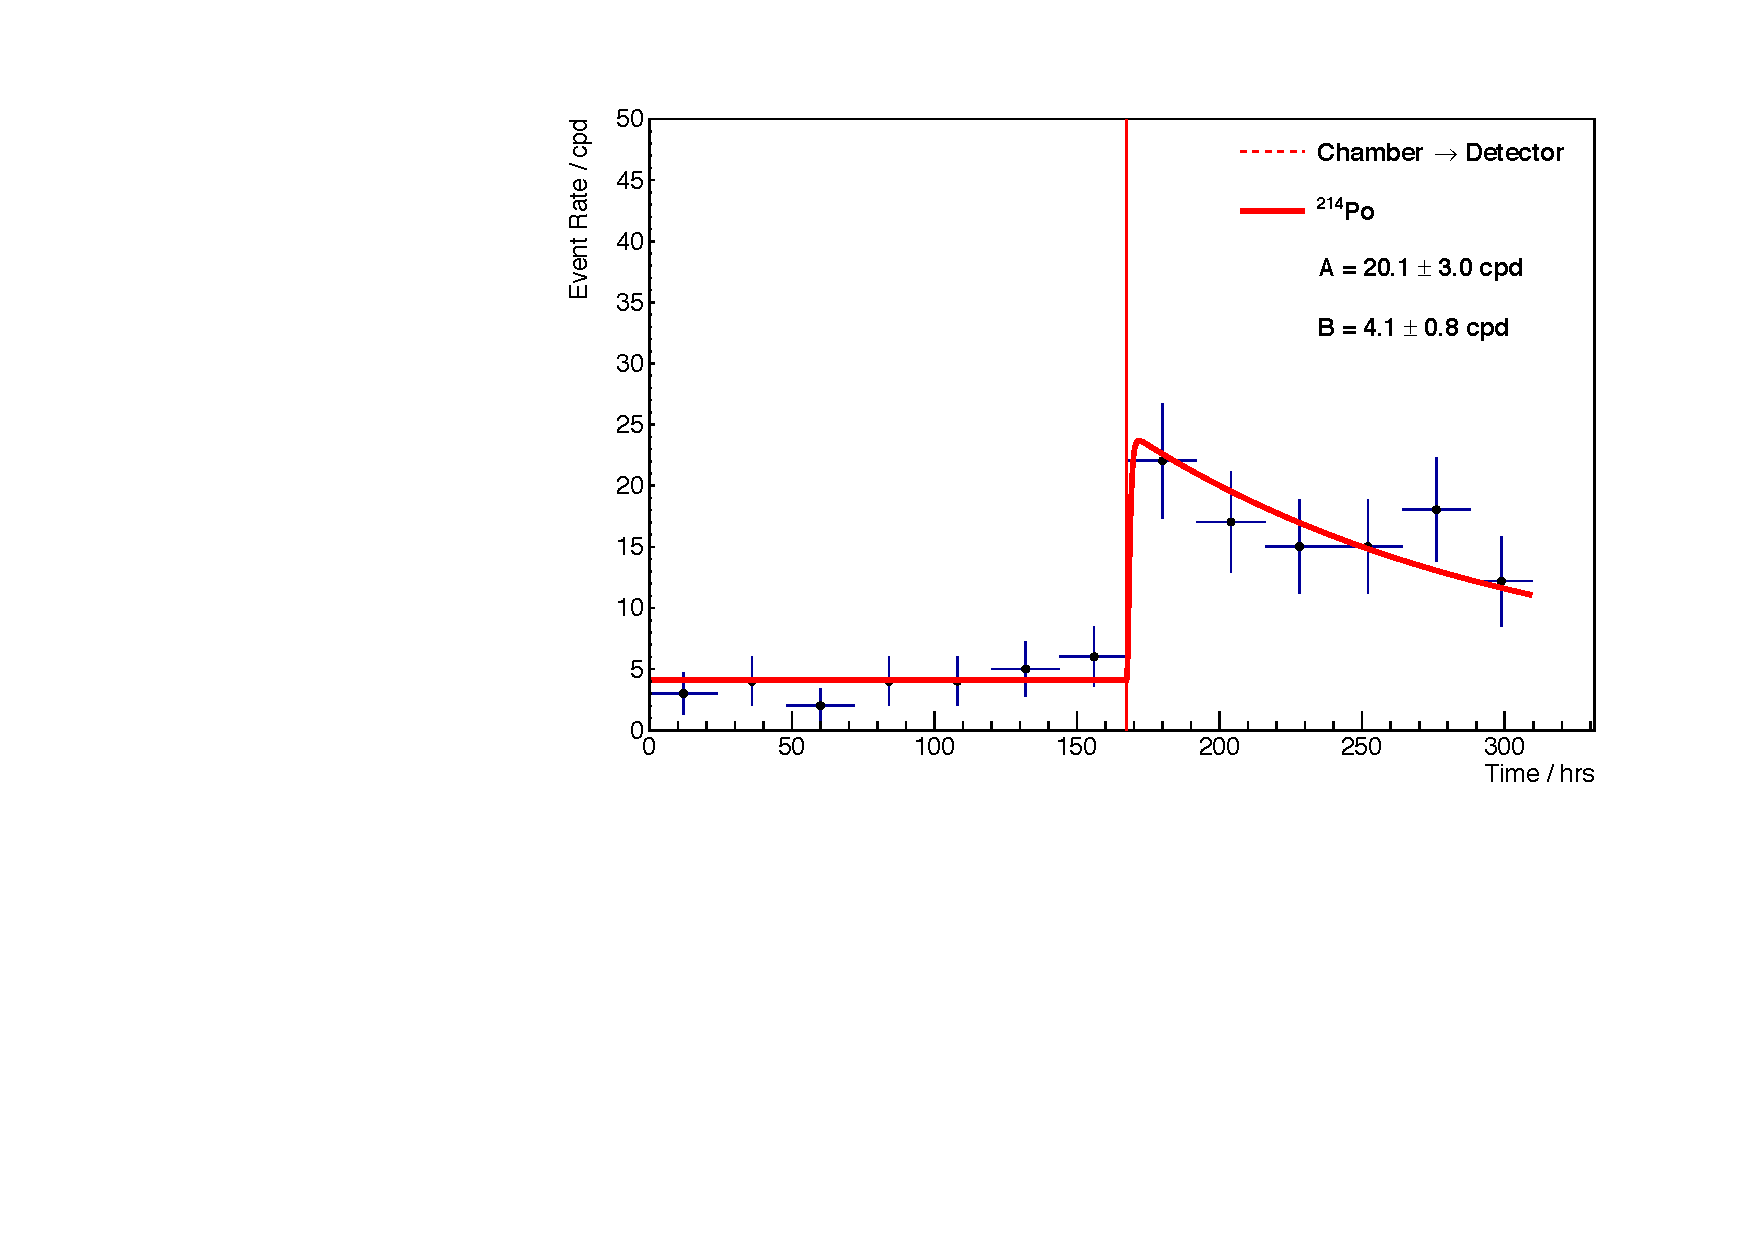
\includegraphics[scale=0.42]{Chapter_4/Figures/ucl_measurements/titanium_sheets_post_etching_2_Po214.pdf}    
    \caption[Pre-corrected \PoTOF{} and \PoTOE{} event rate results obtained from the single measurement made on the pre-etched titanium sheets.]
    {Pre-corrected \PoTOF{} event rate results obtained from the two measurements made on the post-etched titanium sheets.}
    \label{fig:ti_post_etched_sheets_results}
\end{figure}
%

The \PoTOF{} activity measured from the same sample after etching at AstroPak has also shown a signal above the measured background. The two measurements are in good agreement and the averaged rate is calculated to be $685\pm81$ \micro{}Bq. The averaged observed for \PoTOE{} for these two measurements were $476\pm79$ \micro{}Bq. Although there was a clear signal above background, the suppression in comparison to \PoTOF{} still indicates an outgassing induced neutralisation. 

\subsubsection{Discussion \& Conclusion}

The pre- and post-etched emanation rates from the titanium welded block normalised for surface area result in $17.2\pm3.0$ \mBqms and $11.4\pm2.1$ \mBqms, respectively. The surface area normalisation for the titanium sheets for pre- and post-etched measurements give $1.62\pm0.37$ \mBqms and $2.91\pm0.35$ \mBqms, respectively. The titanium results obtained from this study, and for comparison, similar results obtained for stainless steel are highlighted in table \ref{tab:titanium_results}.

The findings from these measurements are unexpected and surprising. The initial expectation for emanation from the titanium was in the order of that measured for stainless steel, but despite the etching, the titanium results in an activity that is $\sim3$ orders of magnitude higher. A small reduction in activity is observed on the titanium welding post etching, but this effect is reversed for the raw titanium sheets, were the activity rises; thus suggesting an ineffectiveness of the etching process on metallic surfaces. Recent results published by the XENON1T collaboration also seem to indicate relatively high emanation rates for titanium. The untreated titanium sheets measured by XENON1T (supplied from Nitronit) are in good agreement with the emanation rates measured for the LZ titanium \cite{Aprile:2020vmn}. They however demonstrate that electropolishing of the titanium surface and removing $\sim30$ $\micro$m from the surface, eliminates all of the measured activity, indicating that the emanation rate is predominantly due to a form of surface contamination. Although electropolishing is known to be a very effective way of removing surface contamination, the size of the LZ detector restricted the use of this technique---leading to alternative forms of etching. 

The total titanium surface within the ICV is 15.1 m\squared{} and a further 0.66 m\squared{} of titanium welding is present in multiple locations. Scaling the etched results from this study to the ICV results in a total emanation rate of $43.9\pm5.3$ mBq and $7.5\pm1.4$ mBq at room temperature for the raw titanium and welded surfaces respectively. For comparison, the bottom-up radon emanation projection prior to the titanium measurement was $\sim20$ mBq from the entire detector. Applying the cross-calibration correction of the UCL detector results in $28.7\pm3.5$ mBq and $4.9\pm0.9$.
%
\begin{table}[h!]
\centering
\caption
[Radon emanation results as obtained from the UCL system for the titanium welded block and titanium sheet assays.]
{Radon emanation results as obtained from the UCL system for the titanium welded block and titanium sheet assays. The results do not take into account the cross-calibration systematic of the UCL detector. For comparison, radon emanation results of titanium (middle rows) and stainless steel welding and foil (bottom rows) are provided, as measured by the XENON1T$^{1}$ collaborations \cite{Aprile:2020vmn} and the GERDA$^{2}$ \cite{osti_20719228, ZUZEL2009889}, respectively.}
\label{tab:titanium_results}
\vspace{1mm}
\renewcommand{\arraystretch}{1.2}
    \begin{tabularx}{1\linewidth}{@{\extracolsep{\fill}}lll}
    \toprule
    
    \textbf{Sample Description} & %1
    \textbf{\RnTTT{} emanation rate} & %2
    \textbf{} & %3
    
    \hline
    \hline
    Titanium welded block (untreated) & $17.2\pm3.0$  & \mBqms{} \\
    Titanium welded block (etched)      & $11.4\pm2.1$  & \mBqms{} \\
    Titanium sheets (untreated)       & $1.62\pm0.37$ & \mBqms{} \\
    Titanium sheets (etched)            & $2.91\pm0.35$ & \mBqms{} \\    

    \hline
    Titanium sheets$^{1}$ (untreated)       & $2.81\pm0.19$ & \mBqms{} \\
    Titanium sheets$^{1}$ (electropolished)       & $<80$ & \uBqms \\
    
    \hline
    Steel welds$^{2}$ (untreated)                   & $0.24\pm0.03$ & \mBqms{} \\   
    Steel welds$^{2}$ (etched \& passivated)          & < 0.1         & \mBqms{} \\
    Stainless steel foil$^{2}$ (untreated)          & $10.2\pm0.8$  & \uBqms{} \\
    Stainless steel foil$^{2}$ (etched \& passivated) & $4.6\pm0.9$   & \uBqms{} \\
    \bottomrule
    \end{tabularx}
\end{table}
%


\subsection{Other Measurements}
\label{secsec:other_emanation}

The UCL radon facility has been used to assay several other components for the LZ experiment. The procedure followed for these assays are identical to those detailed in the former sections. Samples are initially cleaned by cleanroom approved wet wipes prior to the placement into the emanation chamber and left to emanate for $\sim2$ weeks. One week of background data is recorded prior to each transfer and the background rate is subtracted from any observed signal. Results from these measurements are summarised in table \ref{tab:ucl_emanation_results}.

\subsubsection{Cirlex PCBs}

The Cirlex boards screened here are from the same batch of material to those assayed in section \ref{secsec:pmt_base_emanation}, but without all of the electronic components highlighted in table \ref{tab:pmt_base_components}. In an effort to distinguish the radon emanating out of the Cirlex alone a total of 124 3" and 7 1" PCBs, totalling 421 grams were assayed twice. The averaged rate was determined to be $636\pm77$ \micro{}Bq, equating to $1.51\pm0.18$ \micro{}Bq/g. 

\subsubsection{HV Components}

A mixture of HV components were assayed at UCL including; 90" peek rods, 4.5 feet polyethylene tubes, 18 polyethylene displacer discs, 9 feet of fluorinated ethylene propylene (FEP) and 54 polyethylene insulating boomerangs, each provided at a quantity 1.5 times more than required by the LZ detector. Although the activity of the individual components cannot be quantified, an emanation rate of $369\pm85$ \micro{}Bq were measured for the entire batch. 

\subsubsection{DB25s}

As part of the radon screening campaign for the excess ICV radon, a pair of DB25s were assayed. These items were temporarily used in the ICV during the skin installation and hence was an unaccounted item. The measurements resulted in an upper limit of <0.13 mBq.

\subsubsection{Nitrile O-rings}

A total of 90 nitrile rubber o-rings were assayed. The total surface area of the assayed rings were 9.15 cm\squared{}. An emanation rate of $17.6\pm1.7$ mBq was measured per ring. LZ will use a total of 2 nitrile rubber o-rings. 

\subsubsection{Polyoxymethylene (Delrin) Discs}

A collection of 50 Delrin discs with a total surface area of 0.54 m\squared{} was assayed for radon emanation. An emanation rate of $450\pm11$ \uBqms was measured. LZ requires a total of 200 cm\squared{} as part of the installation of the HV umbilical cord, resulting in a contribution of $9\pm2$ \micro{}Bq.


\subsubsection{Titanium Rods}

As part of the radon emanation cross-calibration campaign of the four facilities used by LZ, a set of titanium rods were procured and screened at the various facilitates. A total of 20 rods, 16 cm in lenth and 1 mm in diameter were screened along two small aluminium plates used for structural support. The emanation rate for the sample was measured at $404\pm98$ \micro{}Bq. 


\subsubsection{Summary of Emanation Results}

A summary table of the key measurements made by the UCL system are provided in table \ref{tab:ucl_emanation_results}. The results are provided in easily scalable units for future use and multiple measurements are combined to a single emanation rate. 
%
\begin{table}[h!]
\centering
\caption{Radon emanation results as obtained from the UCL system for all the components measured for the LZ experiment. These results do not include the cross-calibration correction ratio of 1.53.}
\label{tab:ucl_emanation_results}
\vspace{1mm}
\renewcommand{\arraystretch}{1.2}
    \begin{tabularx}{1\linewidth}{@{\extracolsep{\fill}}lll}
    \toprule
    \textbf{Sample Description} & %1
    \textbf{\RnTTT{} emanation rate} & %2
    \textbf{} & %3
    \hline
    \hline
    Titanium welded block (not treated) & $17.2\pm3.0$  & \mBqms{} \\
    Titanium welded block (etched)      & $11.4\pm2.1$  & \mBqms{} \\
    Titanium sheets (not treated)       & $1.62\pm0.37$ & \mBqms{} \\
    Titanium sheets (etched)            & $2.91\pm0.35$ & \mBqms{} \\  
    1" PMT Bases                        & $4.42\pm0.90$ & \micro{}Bq/base \\ 
    3" PMT Bases                        & $5.33\pm0.63$ & \micro{}Bq/base \\ 
    Cirlex PCBs                         & $1.51\pm0.18$ & \micro{}Bq/g \\ 
    HV Components                       & $369\pm85$    & \micro{}Bq/batch \\ 
    DB25s                               & $<0.13$    & \micro{}Bq/unit \\ 
    O-rings (Nitrile)                   & $17.6\pm1.7$    & \micro{}Bq/ring \\ 
    Polyoxymethylene (Delrin) Discs     & $450\pm11$    & \uBqms{} \\ 
    Titanium Rods ($\times$20, L=16 cm, D=1 mm)    & $404\pm98$    & \micro{}Bq \\ 
    \bottomrule
    \end{tabularx}
\end{table}
%


%%------------------------------$$
\section{Other Radon Emanation Assays for LZ}
\label{sec:otherradon}
%%------------------------------$$

The LZ radon emanation screening campaign utilises on four different facilities in measuring small and large scale samples: the UCL facility as detailed in section \ref{sec:ucl_radon_system}, South Dakota School of Mines and Technology (SDSM&T), University of Maryland and University of Alabama facilities. More in-depth discussion and details on these facilities and their operational methods are highlighted in \cite{lz_screening}.

The facilities operate under similar approaches in measuring emanation rates, where samples are initially enclosed in air-tight emanation chambers and the radon is harvested into their respective detectors after the equilibrium period. SDSM\&T and Maryland facilities make use of electrostatic PIN-diode detectors to measure the \alpha-particles from the \PoTOF{} and \PoTOE{} isotopes to reconstruct the radon emanation rate. The Alabama facility operates an organic liquid scintillator detector with a low-activity 3" Hamamatsu R-1307 PMT. Boil-off nitrogen with low intrinsic radon content is used to transfer the radon from an emanation chamber into 150 mL of scintillator. The emanation rate is reconstructed by detecting the scintillation light from the delayed \BiTOF-\PoTOF{} coincidences. 

LZ also makes use of two portable radon collection systems for equipment that is too large or are part of the construction in the SURF Surface Assembly Laboratory (SAL); i.e. radon emanation measurements from the ICV post skin region and TPC installation. Emanated radon is transferred to a cold trap consisting of copper beads or wool that is double-sealed and then transported by car or overnight shipping to the radon facility at SDSM\&T or University of Maryland. The collected radon is then transferred over into the respective radon detector with transfer efficiencies taken into account from portable-system specific calibrations. The activity is then reconstructed by correcting for the transportation time, transfer and detector efficiency. These portable systems were critical for measurements of radon emanation from the assembled LZ detector and from large instrumentation used in the circulation path. Harvesting of radon from the getter system at the SAL using one of the portable systems is displayed on figure \ref{fig:portable_radon_harvesting_system}.
%
\begin{figure}[b]
    \centering
    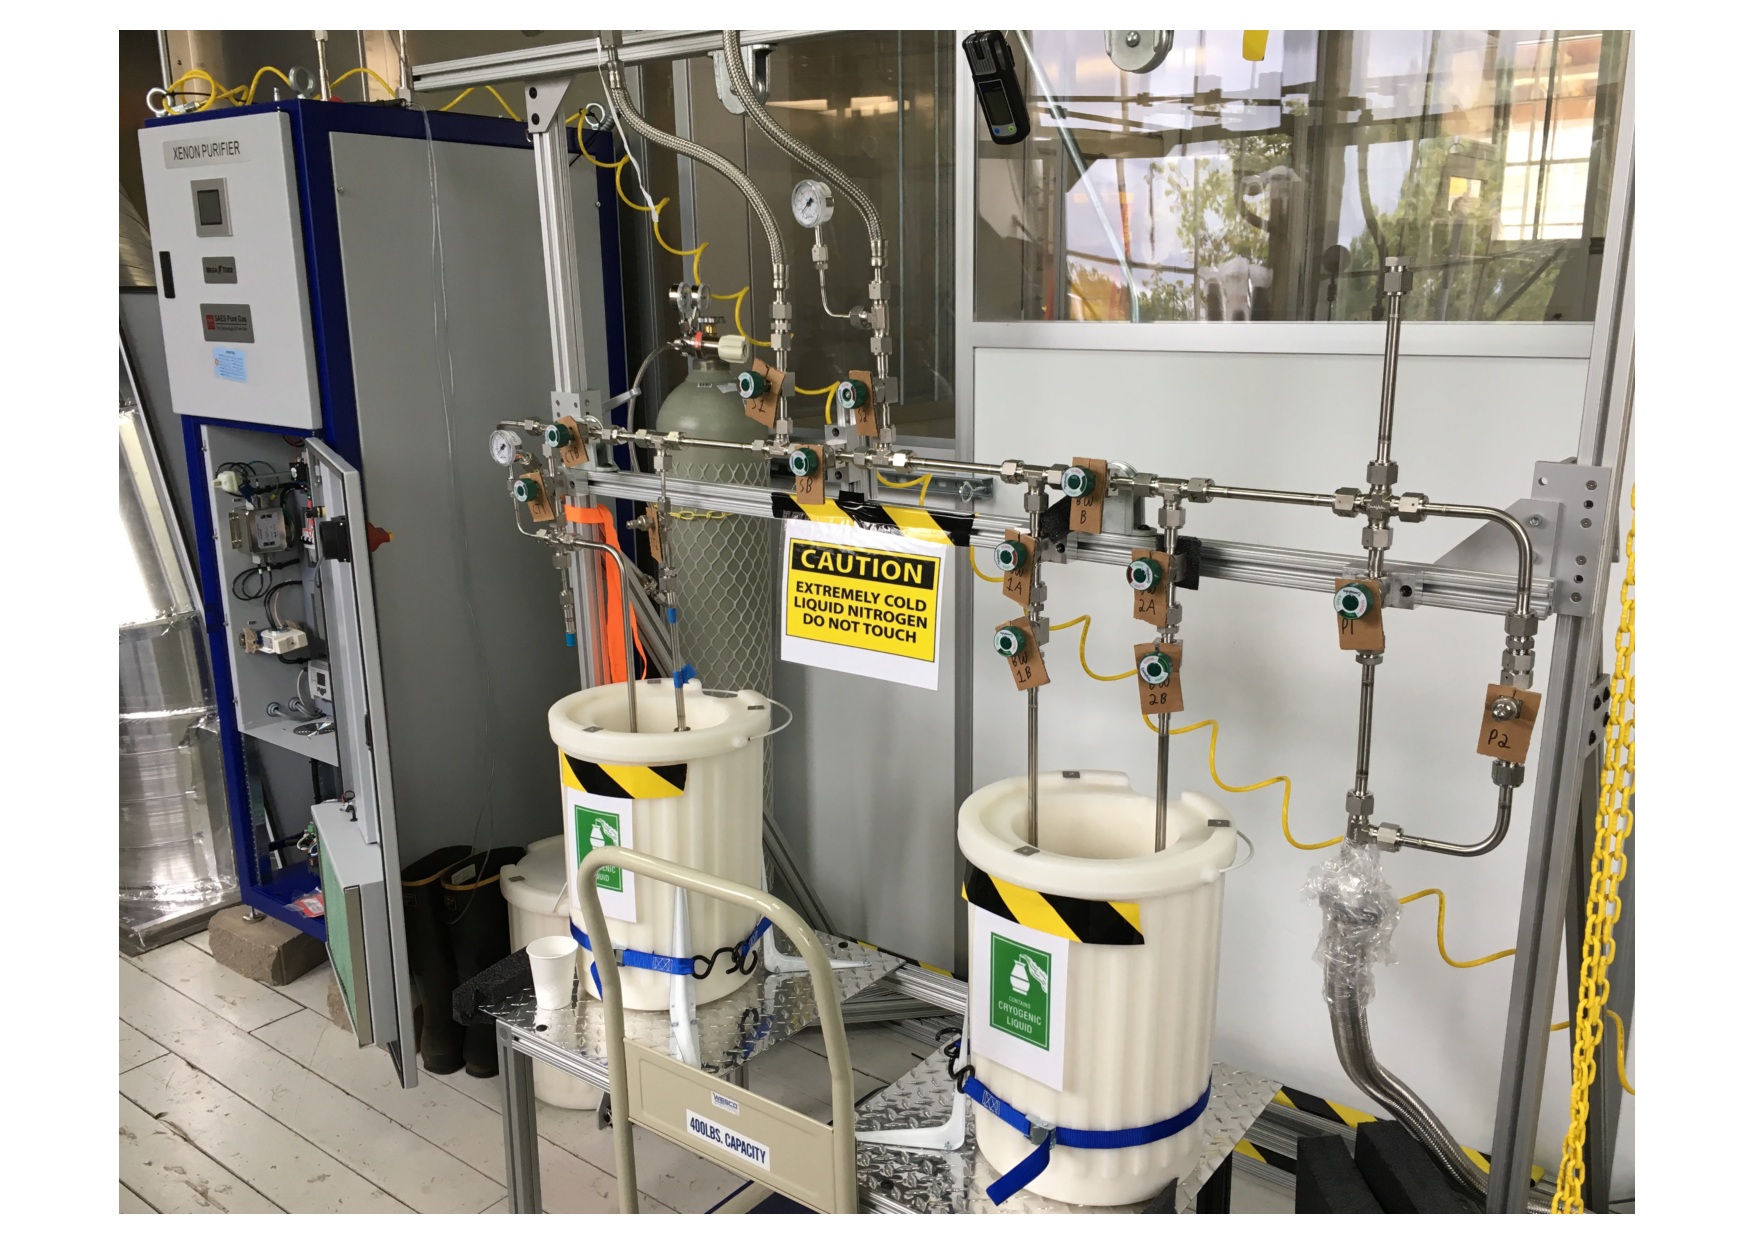
\includegraphics[scale=0.45]{Chapter_4/Figures/portable_system_operation.pdf}
    \caption[A pictorial diagram of the portable radon harvesting system used at the SAL for the getter radon emanation measurement.]
    {A pictorial diagram of the portable radon harvesting system used at the SAL for the getter radon emanation measurement. The emanated radon is collected by transferring through one of the traps held under LN$_{2}$ temperature. The trap is later transported to a radon emanation facility for counting.}
    \label{fig:portable_radon_harvesting_system}
\end{figure}
%


\subsection{Cross-Calibration Campaign}
\label{secsec:cross_cal}

%% NEEDS EDITING
The LZ collaboration performed cross-calibrations for the four radon facilities deployed as part of the assay program. A rubber sample previously screened by the EXO collaboration~\cite{Albert:2015nta, Miller:2017tpl} was assayed at each of the radon emanation facilities. Prior to the emanation period, the sample was prepared under the same conditions to reduce the chances of environmental contamination. The surface of the sample was scrubbed with isopropyl alcohol-soaked lint-free wipes and inspected with UV-light to ensure no presence of surface contamination. The activity of the sample was $\BigOSI{10}{\mBq}$ and was thus well above the minimal detectable activities of the radon systems. Table \ref{tab:ReDet} presents the results of the cross-calibration and a summary of key details of the LZ radon screening facilities. The EXO emanation results indicated an activity of $4.94\pm0.07$ mBq. The cross-calibration results are provided as a ratio between the EXO activity and that measured with the various systems. All but the UCL emanation system agrees with the EXO results within error.
%
\begin{table}[hb!]
    \centering
    \caption{Comparison of the key highlights of the four radon emanation facilities used by LZ. The chambers detailed are those used in containing the sample material, where radon is collected. Some facilities operate two chambers as detailed below. Chamber blank rates detail the emanation rate from the chambers alone and are background subtracted for sample measurements. Detector efficiency represents the fraction of activity measured from the total radon inside the detecting volume; independent of chamber usage and transfer efficiency. The cross-calibration figures represent the reconstructed emanation rate of a standard rubber sample previously used by other collaborations. When not stated, overall uncertainties are estimated to be 10-20\%.}
    \label{tab:ReDet}
    \begin{adjustbox}{width=\textwidth,center}
    \tabcolsep=4pt
        \begin{tabular}{lcccccc}
        \toprule
        \multicolumn{1}{c}{\textbf{Detector}} & %0
        \textbf{Type} & %1
        \multirow{1}{*}{\textbf{Chamber Volumes}} &  %2
        \multirow{1}{*}{\textbf{Chamber Blank Rates}} &  %3
        \multirow{1}{*}{\textbf{Transfer Efficiency}} & %4
        \multirow{1}{*}{\textbf{Detector Efficiency}} & %5
        \multirow{1}{*}{\textbf{Cross-Calibration}}\\ %6
        & %0
        & %1
        \multirow{1}{*}{\textbf{[L]}} & %2
        \multirow{1}{*}{\textbf{[mBq]}} & %3
        \multirow{1}{*}{\textbf{[\%]}} & %4
        \multirow{1}{*}{\textbf{[\%]}} & %5
        \multirow{1}{*}{\textbf{[Measured/EXO--activity]}}\\ %6
        \hline
        \hline
        \vspace{-4mm}
        \\ 
        SDSM\&T & 
        PIN-diode & 
        \multicolumn{1}{c}{\begin{tabular}[c]{@{}c@{}}13\\ 300\end{tabular}} & \multicolumn{1}{c}{\begin{tabular}[c]{@{}c@{}}0.2\\ 0.2\end{tabular}} & 
        \multicolumn{1}{c}{\begin{tabular}[c]{@{}c@{}}94\\ 80\end{tabular}} & 
        25 & 
        \multicolumn{1}{c}{\begin{tabular}[c]{@{}c@{}}0.89$\pm$0.15\\ 1.11$\pm$0.28\end{tabular}}
        \vspace{2mm}
        \\ 
        Maryland & 
        PIN-diode & 
        4.7 & 
        0.2 & 
        96 & 
        24 & 
        1.13 $\pm$ 0.19
        \vspace{2mm} \\
        UCL & 
        PIN-diode & 
        \multicolumn{1}{c}{\begin{tabular}[c]{@{}c@{}}2.6\\ 2.6\end{tabular}} &
        \multicolumn{1}{c}{\begin{tabular}[c]{@{}c@{}}0.2\\ 0.4\end{tabular}} & 
        \multicolumn{1}{c}{\begin{tabular}[c]{@{}c@{}}97\\ 97\end{tabular}} & 
        30 & 
        1.53$\pm$0.15
        \vspace{2mm} \\ 
        Alabama & 
        Liquid Scint. & 
        \multicolumn{1}{c}{\begin{tabular}[c]{@{}c@{}}2.6\\ 2.6\end{tabular}} &
        \textless{}0.4 & 
        34 &
        36 & 
        0.83$\pm$0.17
        \\
        \bottomrule
        \end{tabular}
    \end{adjustbox}
\end{table}
%

There are several considerations for the discrepancy for the unknown systematic observed for the UCL system. Due to the size and geometry of the sample, the transfer efficiency from the chamber may be overestimated, as some radon may have been trapped in folded pockets of the rubber sample. The UCL system transfers the chamber content with 10 times the volume of the chamber; hence it is difficult to explain such a large discrepancy with this explanation alone. Another explanation could be the exposure of the sample to radium rich air, hence increasing the radon activity of the sample. Due to the uncertainties in understanding why the UCL system is behaving in such a way, it is difficult to conclusively explain this behavior and further tests will be conducted between the LZ radon emanation systems to fully understand if such an upwards systematic exists. 


\subsection{Large Scale Radon Emanation Studies}
\label{secsec:large_scale_measurements}

Room temperature measurements from individual material and components measured by various radon facilities are all presented in \cite{lz_screening}. Furthermore, measurements from fully assembled sub-systems, such as the ICV, xenon purification and circulation system are also presented in figure \ref{LZ_radon_diagram_paper}. Measurements for three of these assemblies are discussed in the following sub-sections. These measurements were made possible by the portable radon harvesting system deployed at SURF. 

\subsubsection{Inner Cryostat Vessel}

Radon emanation from the ICV was measured several times during various integration stages of the construction of the skin veto region and the TPC installation. The final assay was made following after the ICV was fully complete and sealed. The cryostat at this stage housed both the top and the bottom PMT arrays for the TPC and the skin veto regions, and their corresponding PMT bases and cables. Furthermore, the entire field cage, PTFE coating, various sensors, and conduit volumes of the cables were a part of these measurement.

A portable radon trapping system was deployed underground at SURF with minimal plumbing due to space constraints. After leak-checking and purging, the trapping system was opened to the ICV and the emanated gas was harvested over a 6.3 hour period---equivalent to 18.25\% of the gas within the ICV. After the harvest, the trap was carefully disconnected and transported to SDSM\&T radon facility for screening. The radon trap also captures outgassing molecular species that would serve as neutralisers of positively charged radon-daughters, leading to a drop in detection efficiency. An in-house procedure was followed to separate out these species by transferring the sample from a cold trap held at -109$^{\circ{}}$C to one at -196$^{\circ{}}$C with sufficient flow to effectively transfer all of the radon atoms while leaving most of the contaminants behind. This process was repeated until measurements with a residual gas analyzer indicated no further reduction in contaminant concentration, after which the sample was transferred to the detection chamber via a secondary small cold trap. Results indicate a room-temperature emanation rate of $46.1^{+4.0}_{-3.8}\,$mBq under the assumption of an even sampling of the radon within the ICV.


\subsubsection{Xenon Circulation System}

The xenon gas circulation system brings together multiple components and surfaces that are potential radon emitters. The system consists of two gas compressors, a heated zirconium getter, and a main valve and instrumentation panel. The compressors (model A2-5/15 from Fluitron) have two heads, each enclosing a flexible all-metal diaphragm sealed with copper plating. Check valves, accumulation bottles, and associated plumbing and instrumentation are also included in the compressor assemblies. The compressors operate in parallel to achieve a gas flow rate of 500 standard liters per minute. Much of the system was fabricated at the University of Wisconsin's Physical Sciences Laboratory. Whilst there, a portable radon trapping system was used to harvest emanation samples that were then shipped to shipped to the U. Maryland radon facility for counting.

Initial radon emanation measurements of compressor 2 found that the heads emanated \SI{< 1}{\milli\becquerel} each, however, the integrated compressor skid assembly presented $\sim$\SI{17}{\milli\becquerel}. After replacing most of the welded stainless steel plumbing and etching the accumulation bottles in citric acid, the rate was reduced to $1.48\pm0.31$\,mBq. A similar treatment was applied to compressor 1 but this compressor was not radon emanated and hence is assumed to have the same rate as compressor 2. The main circulation panel contains most of the valves and instrumentation exposed to the xenon in gas phase, and it was found to contribute \SI{0.74}{\milli\becquerel} of radon. The fully loaded getter (model PS5-MGT50-R-535 from SAES) was emanated at its operational temperature of $400 ^{\circ}$C using helium carrier gas and its emanation rate was determined to be \SI{2.26}{\milli\becquerel}. The entire circulation system amounted to a total emanation rate of $5.22\pm0.75$\,mBq.


\subsubsection{Xenon Tower}

The xenon tower is a cryogenic system that thermally couples the gaseous and LXe portions of the purification circuit for efficient heat transfer, serving to vaporize and re-condense the liquid for continuous purification. It consists of a two-phase heat exchanger (supplied from Standard Xchange), three cryogenic valves (manufactured by WAKE), a sub-cooler/phase-separator vessel to hold LXe returning to the detector, a reservoir vessel to hold liquid exiting the detector, two liquid xenon purity monitors, and several custom liquid xenon heat exchangers. The tower can be viewed as having two sides: the heat exchanger assembly on one side and the weir reservoir, sub-cooler and purity monitor on the other. Radon emanation from sub-components was measured prior to full integration of the xenon tower and was found to contribute a total of \SI{<1}{\milli\becquerel}. 

A preliminary measurement of the tower after integration found a very high radon activity in the reservoir side, possibly due to a leak into the system from laboratory air. As a precautionary measure, the reservoir vessel was flushed with a concentrated solution designed for removing radioactive contamination (Radiacwash\textsuperscript{TM}) and rinsed with deionized water. The portable radon trap was then deployed underground to measure the two sides of the complete xenon tower prior to the installation of the purity monitor and found a total emanation rate of $3.14^{+0.86}_{-0.81}$\,mBq.


%%------------------------------$$
\section{Radon Emanation Projection in LZ}
\label{sec:lzradon}
%%------------------------------$$

Sensitivity projections for LZ presented in \cite{akerib2018projected} include the effect of the online charcoal-based radon-removal system, operating continuously to scrub gaseous Xe \cite{lz_tdr, Pushkin:2018wdl}. Although this system will not scrub majority of the xenon within the ICV, a volumetric gas flow of 2 slpm has been shown to eliminate 90\% of the radon from cables and feedthroughs. LZ will utilise on a 7.0 kg charcoal trap to reduce radon emanation from instrumentation immersed in GXe; particularly, radon emanation from the top PMT array, cabling and sensors, along with all the titanium surfaces on the upper-side of the ICV. 

Projections also assume an expected suppression of radon diffusion in certain materials at low temperatures, namely those suspended within the LXe were the operational temperature is 175.8 K (-97.4$^{\circ{}}$C). Its important to note that the radon emanation assays from all the samples---whether individual components screened using emanation chambers, or system-wide instrumentation's screened using a portable harvesting system---were all performed at room temperature (\sim{}20$^{\circ{}}$C).

The projection of radon emanation from warm measurements to operational conditions is a difficult task involving multiple assumptions and approaches. In calculating an operational rate, both the radon reduction system and the suppression due to cold temperature has to be taken into account. The ratio of components sitting within the operational volume of the radon reduction system is well known, but there are still many uncertainties on the suppression rates obtained at cold temperature. Furthermore, these rates heavily depend on the type of material used; more emanation reduction is expected from porous materials like plastics and ceramics when cold. The sections below will initially construct a warm emanation rate projection of the entire detector, and a further attempt to quantify operational rates through literature-based educated assumptions on suppression.  


\subsection{Bottom-up Projection}

Prior to large scale emanation results during construction, the radon projection was constructed entirely from a bottom-up approach from measuring components and material in fractional quantities and scaling the emanation results to quantities present in LZ. The results from this approach with various projections are detailed in table \ref{tab:lz_bottom_up_results}.

Although the table does not fully account for all of the items to be used in LZ, majority of the radon contributors are included. Components such as sensors and screws have previously been emanated but contribute negligible amounts to the total sum. The results obtained by UCL, i.e., the raw titanium, titanium welding and PMT base results, take into account the systematic correction of 1.53 from cross-calibrations. Components that are within the operational ground of the radon removal system are further suppressed by the previously determined 90\% removal efficiency. The GXe suppression factor therefore is $S=0.1$, where the LXe suppression factors are component specific: $S1=0.5,\;S2=0.1,\;S3=0.01,\;S4=0.001,\;S5=0.0001$. The cold reduction values for plastics (S3, S4, S5) originate from diffusivity data on Kapton, Acrylic and PTFE; where temperature dependence of diffusivities of Ar and Kr were evaluated from \cite{Schowalter_2010} by the EXO collaboration and a model for radon is constructed. Components using mixtures of material---such as the bases---use a conservative suppression value ($S2$); though its important to note that the majority of the emanation is from Cirlex ($\rho{}\simeq{}1.42$g/cm$^{3}$), which has a similar density as PTFE ($\rho{}\simeq{}2.2$g/cm$^{3}$). 

Finally, ($S1$) is used for components with metallic surfaces; i.e. PMTs, but more importantly the titanium welding and cryostat. Material such as glass and metals are crystalline in nature and hence space for additional atoms is often limited, especially for the large radon atom. Hence diffusion through such material is suppressed as a nature of the material, as radon would then have to displace or significantly deform the lattice structure to squeeze through, which is heavily suppressed at room temperature. In such a case, emanation is dominated by recoil and hence no suppression at colder temperatures. However, this assumption only applies to perfect lattice structure. The lattice formation depends heavily on the cooling methods when forming the solid metal. A slow cooling process can lead to large crystalline grain formations, whereas a fast cooling process leads to small grains. The grain boundaries represent a surface of imperfect lattice that could be a route for radon to diffuse. 

The expected radon emanation from the LZ detector that emanates directly into volumes in line with the GXe and LXe without any suppression factors result in a rate of $60.8^{6.0}_{-6.1}$ mBq. Although not detailed in table \ref{tab:lz_bottom_up_results}, by taking only into account the suppression from the radon removal system and omitting any cold suppression, an emanation rate of $41.3^{+4.4}_{-4.5}$ mBq is obtained. Taking into account the conservative cold suppression factors in table \ref{tab:lz_bottom_up_results}, this rate further drops to $21.6^{+2.3}_{-2.3}$ mBq. If a substantial amount of emanation from the cryostat and the welding is as a result of diffusion, a significant suppression due to cold could be expected. To reflect this, the conservative ($S1$) suppression factor was substituted with ($S2$), giving a total expected emanation rate of $11.0^{+1.0}_{-1.0}$ mBq for an optimistic scenario. The LZ detector is expected to take commissioning data operating fully in GXe and with LXe, hence the comparison of that data to estimations presented here is of utmost interest.

\subsection{Large Scale Assay Projections}

A second method to estimate for the total radon in LZ was by using the large scale measurements highlighted in section \ref{secsec:large_scale_measurements}. Results obtained using this method for the sub-systems of interest is provided in figure \ref{LZ_radon_diagram_paper}. The main difference here is that the entire ICV and the xenon tower has been emanated after the installation of all sub-components. The comparison between large-scale and bottom-up ICV measurements obtained from table \ref{tab:lz_bottom_up_results}, result in a remarkably good agreement, with $46.1^{+4.0}_{-3.8}$ mBq and $48.5^{+5.9}_{-6.0}$ mBq, respectively. Combining the outcomes of the large-scale measurements result in a total emanation rate of $60.4^{+4.2}_{-4.0}$ mBq for the LZ experiment, which in good agreement with the bottom-up estimations when excluding suppression factors.


\subsection{Discussion}

The results obtained from bottom-up assays and large scale emanation measurements during sub-system installation at the SAL are in good agreement within error. A large proportion of the emanation rate is expected from the ICV, of which, the largest contribution comes from the cryostat, welding and the PMT-base pairings. The emanation rate measured from the cryostat titanium was unexpected. Exclusion of the titanium emanation rate from the bottom-up ICV results lead to a substantial underestimation of the emanation rate when compared to the large-scale ICV result. Furthermore, the issue around the UCL systematic adds another layer of complexity, but it is safe to say that this factor is indeed a systematic and not a result of external circumstances. This conclusion is reached when considering the comparison between the ICV bottom-up and total; if this correction was not applied, the bottom-up scenario will substantially overestimate the result from the complete ICV emanation. The agreement between the large scale emanation results and that of the bottom-up adds further confidence to the cross-calibration factor used to estimate radon emanation at operational conditions. Assuming the fraction of radon emanation coming from each sub-component is accurate and the suppression factors are conservative; the worst case scenario with only the radon removal suppression yields an emanation rate of $41.3^{+4.4}_{-4.5}$ mBq. This further reduces to $21.6^{+2.3}_{-2.3}$ mBq and $11.0^{+1.0}_{-1.0}$ mBq when less conservative ($S1\rightarrow{}S2$) suppression factors for LXe are successively assumed. Chapter \ref{chap:chap5} will investigate the significance of the radon background for the WIMP search, studying the implications of these scenarios for the sensitivity and the discovery potential of WIMPs.

%
\vspace{1.5cm}
\begin{figure}[h]
    \centering
    \hspace*{-0.2cm}
    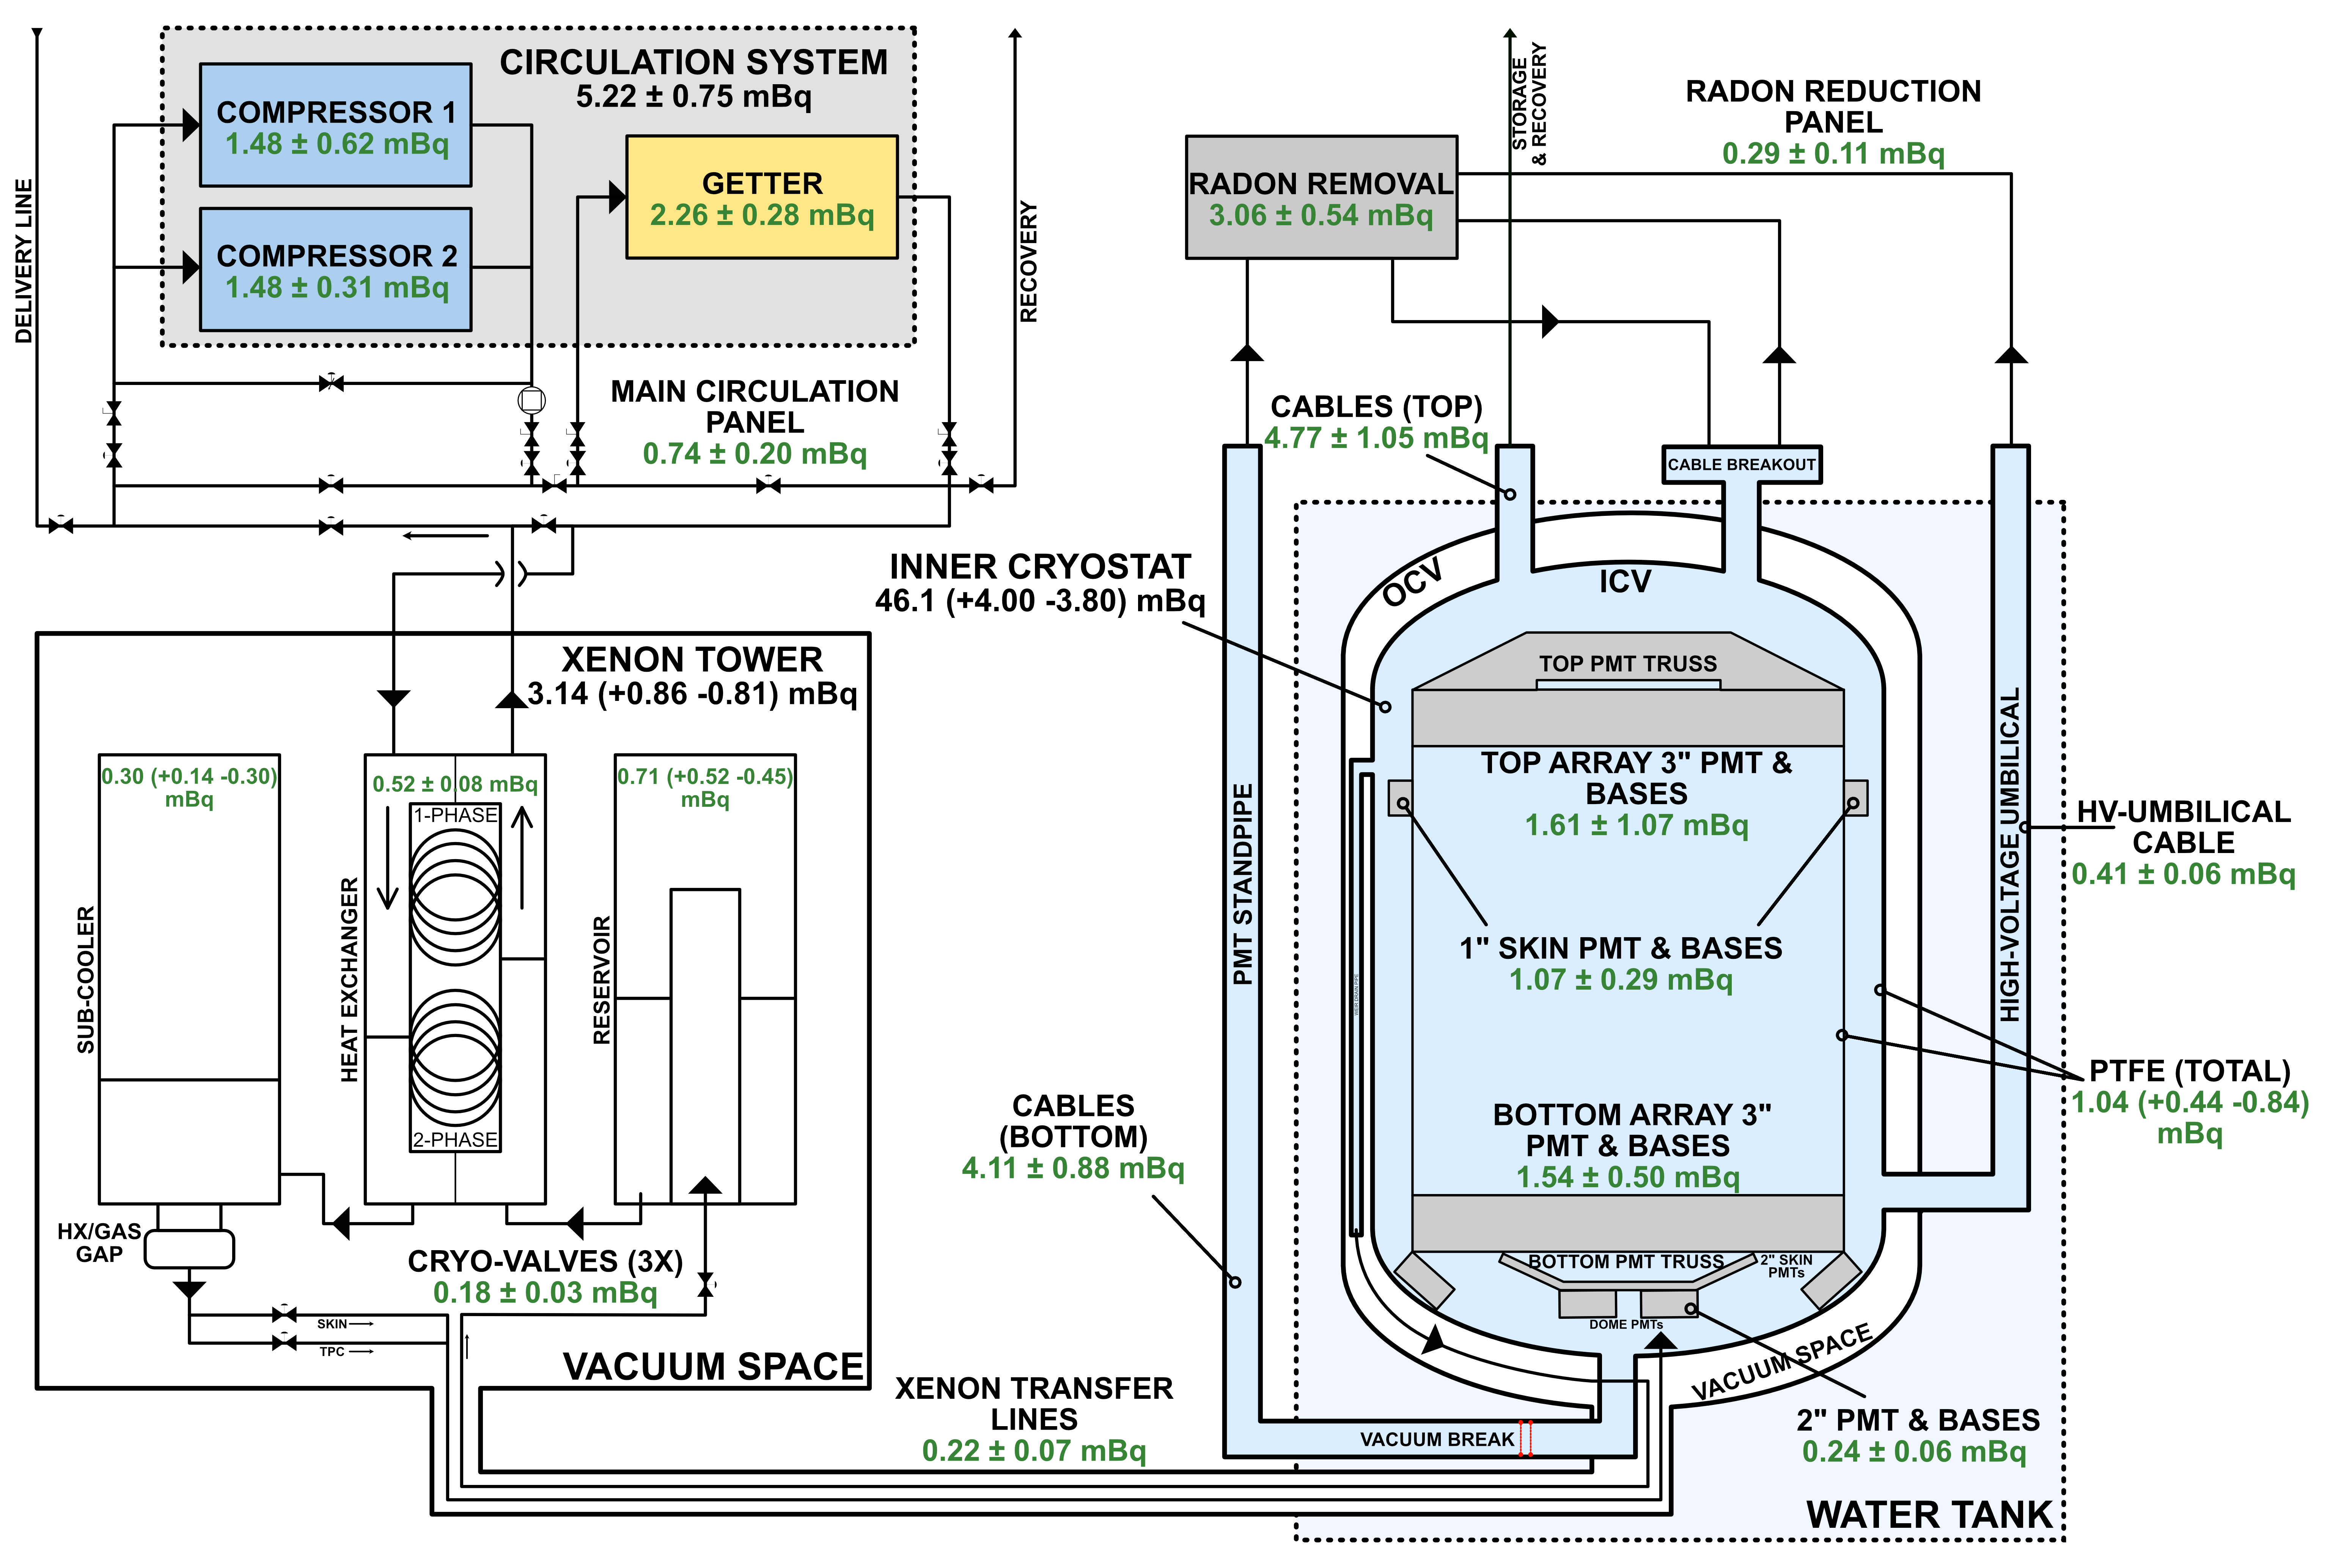
\includegraphics[scale=0.3]{Chapter_4/Figures/LZ_Radon_Diagram_Paper.png}
    \caption
    [Approximate schematic of LZ highlighting key sub-systems and xenon circulation paths in and out of the ICV.]
    {Approximate schematic of LZ highlighting key sub-systems and xenon circulation paths in and out of the ICV. The diagram condenses some of the key radon emanation measurements that will contribute to the overall radon budget of LZ. The results presented in green text are directly from measurements and those in black show summed results for that particular component. All of the results shown are measurements made at room temperature and does not include the cold suppression expected under full operation.}
    \label{LZ_radon_diagram_paper}
\end{figure}
%

%
\begin{table}[p!]
\centering
\caption{Results obtained from component and material radon emanation from various facilities used by LZ. The UCL results provided take into account the systematical fraction highlighted in table (\ref{tab:ReDet}). Provided are the components and quantities used in LZ and emanation results obtained from same/similar samples. Fraction of components occupying either the GXe region of the detector---where radon removal system will operate, or the LXe region---where cold suppression is considered. Emanation rates expected from these two regions after applying the suppression factors is given in the last two columns. The  GXe suppression factor is S=0.1, where the LXe suppression factors are component specific: S1=0.5, S2=0.1, S3=0.01, S4=0.001, S5=0.0001. Those components were neither suppression factor apply are left blank; i.e. xenon tower and circulation. The remaining results from the radon emanation campaign are detailed in \cite{lz_screening}.}
\label{tab:lz_bottom_up_results}
\vspace{1mm}
\renewcommand{\arraystretch}{1.2}
    \begin{adjustbox}{width=\textwidth,center}
    \tabcolsep=4pt
        \begin{tabular}{lcc|cc|cc|cc}
        \toprule
        
        \multicolumn{1}{l}{\textbf{Component}} %1
        & \multicolumn{2}{c|}{\textbf{Quantity}} %2
        & \multicolumn{2}{c|}{\textbf{\RnTTT}} %4
        & \multicolumn{2}{c|}{\textbf{Location [\%]}} %6 
        & \multicolumn{2}{c}{\textbf{Suppression [\micro{}Bq]}} \\ %7 
        
            %1
        &   %2
        &   %3
        &   %4
        &   %5
        & GXe %6
        & LXe %7
        & GXe %8
        & LXe \\ %9
        
        \hline
        \hline
        
        \textbf{ICV} &  &  &  &  &  &  &  &  \\
        
        Titanium (Raw)\textsuperscript{S1} & 15.1 & m\squared & 2910.0$^{+0.4}_{-0.4}$ & \uBqms & 0.25 & 0.75 & 35.90 & 10769.85 \\
        Titanium (Welding)\textsuperscript{S1} & 0.66 & m\squared  & 7451.0$^{+2.1}_{-2.1}$ &	\uBqms & 0.10 &	0.90 & 2.46 & 2212.94 \\
        3" PMTs (R11410)\textsuperscript{S1} & 494 & unit & 1.8$^{+1.7}_{-1.8}$ & \micro{}Bq/unit & 0.51 & 0.49 & 2.28 & 216.96 \\
        PMT Bases (3")\textsuperscript{S2} & 499 & unit & 3.5$^{+0.6}_{-0.6}$ & \micro{}Bq/unit & 0.51 & 0.49 & 4.46 &	84.66 \\
        2" PMT (R8520)\textsuperscript{S1} & 48 & unit & 1.8$^{+1.0}_{-1.3}$ & \micro{}Bq/unit & 0.00 & 1.00 & 0.00	& 43.92 \\
        PMT Bases (2")\textsuperscript{S2} & 49 & unit & 3.5$^{+0.6}_{-0.6}$ & \micro{}Bq/unit & 0.00 & 1.00 & 0.00	& 17.07 \\
        1" PMT (R8778) & 93 & unit & 7.1$^{+2.6}_{-3.0}$ & \micro{}Bq/unit & 1.00 & 0.00 & 3.30 & 0.00 \\
        PMT Bases (1")\textsuperscript{S2} & 94 & unit & 2.9$^{+0.9}_{-0.9}$ & \micro{}Bq/unit & 0.99 &	0.01 & 1.34 & 0.30 \\
        Cables (Axon)\textsuperscript{S4} &	14802 &	m &	0.6$^{+0.1}_{-0.1}$ & \micro{}Bq/m & 0.55 &	0.45 & 24.65 &	4.10 \\
        Cables (Koax)\textsuperscript{S4} &	1771 & m & 0.03$^{+0.23}_{-0.03}$ &	\micro{}Bq/m & 0.70 & 0.30 & 0.16 &	0.01 \\
        PTFE\textsuperscript{S5} & 84 &	m\squared & 12.4$^{+5.3}_{-10.0}$ & \uBqms & 0.00 & 1.00 & 0.00	& 0.10 \\
        Kapton Sheets &	1.25 &	m\squared &	56.0$^{+104.0}_{-56.0}$ & \uBqms & 1.00 & 0.00 & 0.35 &	0.00 \\
        HV Feedthrough & 21 & unit & 37.0$^{+12.0}_{-12.0}$ & \micro{}Bq/unit &	1.00 & 0.00 & 3.89 & 0.00 \\
        Signal Feedhrough &	31 & unit &	23.0$^{+18.0}_{-14.0}$ & \micro{}Bq/unit & 1.00 & 0.00 & 3.57 & 0.00 \\
        Anode/Cathode Feedhrough & 3 &	unit &	18.8$^{+19.0}_{-18.8}$ & \micro{}Bq/unit & 1.00 & 0.00 & 0.28 &	0.00 \\

        \hline
        \textbf{HV Umbilical} &  &  &  &  &  &  &  &  \\
        Umbilical Cable\textsuperscript{S3} & 7.8 &	m &	52.0$^{+8.0}_{-8.0}$ & \micro{}Bq/m & 0.51 & 0.49 & 1.04 &	1.98 \\
        Mixed Components\textsuperscript{S2} & 0.67 & batch & 369.0$^{+85.0}_{-85.0}$ & \micro{}Bq/batch & 0.20 & 0.80 & 0.25 & 19.68 \\
    
        \hline
        \textbf{Radon Removal \& Transfer Lines} &  &  &  &  &  &  &  &  \\
        Activated Carbon (Trap) & 6 & kg & 510.0$^{+90.0}_{-90.0}$ & \micro{}Bq/kg & 1.00 &	0.00 & 400.86 & - \\
        Radon Reduction Panel &	1 & unit & 290.0$^{+110.0}_{-110.0}$ & \micro{}Bq/unit & 1.00 &	0.00 & 1.45 & - \\
        Xenon Transfer Lines & 1 & unit	& 220.0$^{+70.0}_{-70.0}$ &	\micro{}Bq/unit & 0.00 & 1.00 & 0.00 & 220.00 \\

        \hline
        \textbf{Xenon Circulation} &  &  &  &  &  &  &  &  \\
        Purification Getter & 1 & unit & 2260.0$^{+280.0}_{-280.0}$ & \micro{}Bq/unit &	- &	- & 2260.00 & - \\
        Compressors & 2 & unit & 1480.0$^{+310.0}_{-310.0}$ & \micro{}Bq/unit & - & - & 2960.00 & - \\
        Circulation Panel &	1 &	unit & 740.0$^{+200.0}_{-200.0}$ & \micro{}Bq/unit & - & - & 740.00 & - \\   
        
        \hline
        \textbf{Xenon Tower	} &  &  &  &  &  &  &  &  \\
        Xylem HEX &	1 & unit & 529.0$^{+132.0}_{-132.0}$ &	\micro{}Bq/unit & - & - & 529.00 & - \\   
        Subcooler HEX &	1 &	unit & 300.0$^{+140.0}_{-300.0}$ & \micro{}Bq/unit & - & - & 300.00 & - \\   
        WEKA Valves & 3 &	unit & 60.0$^{+10.0}_{-10.0}$ &	\micro{}Bq/unit & - & - & 180.00 & - \\   
        Conditioning Heater &	2 &	unit & 36.0$^{+17.0}_{-15.0}$ & \micro{}Bq/unit & - & - & 72.00 & - \\   
        Misc Others & 1 & batch & 500.0$^{+500.0}_{-500.0}$ & \micro{}Bq/batch & - & - & 500.00 & - \\   
        
        \hline
        \hline
        
        \textbf{Sub-total [mBq]} & & & & & & & \textbf{8.03$^{+0.89}_{-0.93}$} & \textbf{13.6$^{+2.1}_{-2.1}$} \\
        \textbf{Total [mBq]} & & & \textbf{60.8$^{+6.0}_{-6.1}$} &  & & & \multicolumn{2}{c}{\textbf{21.6$^{+2.3}_{-2.3}$}} \\
        
        \bottomrule
        \end{tabular}
    \end{adjustbox}
\end{table}
%